% v2-acmsmall-sample.tex, dated March 6 2012
% This is a sample file for ACM small trim journals
%
% Compilation using 'acmsmall.cls' - version 1.3 (March 2012), Aptara Inc.
% (c) 2010 Association for Computing Machinery (ACM)
%
% Questions/Suggestions/Feedback should be addressed to => "acmtexsupport@aptaracorp.com".
% Users can also go through the FAQs available on the journal's submission webpage.
%
% Steps to compile: latex, bibtex, latex latex
%
% For tracking purposes => this is v1.3 - March 2012

\documentclass[prodmode,acmtoplas]{acmsmall} % Aptara syntax
\usepackage{etex}				% extend latex, especially the number of registers

\usepackage[utf8]{inputenc}
\usepackage[T1]{fontenc} % ou \usepackage[OT1]{fontenc}
\usepackage[frenchb]{babel} % optionnel

\usepackage[dvipsnames]{xcolor}
\usepackage{pgfplots}			% plotting graphs
\pgfplotsset{compat=1.12}
\usetikzlibrary{patterns}

\usepackage{bussproofs}

\graphicspath{{./images/}}
\usepackage[caption=false,font=footnotesize]{subfig}

\usepackage{multirow}
\usepackage{multicol}
\usepackage{array}
\usepackage{amsmath}
\usepackage{mathtools}
\usepackage{listings}
\lstdefinestyle{full}{
	language=C,
	numbers=left,
	captionpos=b,
	breaklines=true,
	frame=single,
	basicstyle=\footnotesize,
	tabsize=2,
	escapeinside={(*}{*)},
	moredelim=**[is][\color{Red}]{@}{@},
	moredelim=**[is][\color{blue}]{@@}{@@},
	moredelim=**[is][\color{Green}]{@@@}{@@@},
	morekeywords={par, weak, abort, when, input, output, shared, pause, combine, all, new, mod, with, status, preempt, copy, nop
		  life, mission, noncritical, Hz,
		  EOT, PAR,
		  ||, signal, module, emit, present, then, end, immediate}
}

\lstdefinestyle{fulltight}{
	language=C,
	numbers=left,
	captionpos=b,
	breaklines=true,
	frame=single,
	basicstyle=\scriptsize\sffamily,
	tabsize=2,
	escapeinside={(*}{*)},
	columns=flexible,
	xleftmargin=20pt,
	moredelim=**[is][\color{Red}]{@@}{@@},
	morekeywords={par, weak, abort, when, input, output, shared, pause, combine, all, new, mod, with, status, preempt, copy, nop
		  life, mission, noncritical, Hz,
		  EOT, PAR,
		  ||, signal, module, emit, present, then, end, immediate}
}

\lstdefinestyle{snippet}{
	language=C,
	basicstyle=\small,
	frame=none,
	captionpos=b,
	numbers=none,
	xleftmargin=16pt,
	breaklines=true,
	tabsize=2,
	escapeinside={(*}{*)},
	morekeywords={par, weak, abort, when, input, output, shared, pause, combine, all, new, mod, with, 
		  life, mission, noncritical, Hz,
		  EOT, PAR,
		  ||, signal, module, emit, present, then, end, immediate}
}

\newcommand{\StateP}{\ensuremath{S}}
\newcommand{\Abort}{\ensuremath{A}}
\newcommand{\abort}{\ensuremath{a}}
\newcommand{\Environment}{\ensuremath{E}}
\newcommand{\Input}{\ensuremath{I}}

\newcommand{\Id}{\ensuremath{\mathit{Id}}}
\newcommand{\id}{\ensuremath{\mathit{id}}}
\newcommand{\Global}{\ensuremath{\mathcal{G}}}
\newcommand{\Store}{\ensuremath{Store}}
\newcommand{\store}{\ensuremath{store}}
\newcommand{\Var}{\ensuremath{Var}}
\newcommand{\var}{\ensuremath{var}}
\newcommand{\Val}{\ensuremath{Val}}
\newcommand{\val}{\ensuremath{v}}
\newcommand{\Sts}{\ensuremath{Sts}}
\newcommand{\sts}{\ensuremath{sts}}
\newcommand{\expression}{\ensuremath{exp}}
\newcommand{\imm}{\ensuremath{imm}}

\newcommand{\thread}[1]{\ensuremath{\mathit{t}_{#1}}}
\newcommand{\Thread}{\ensuremath{T}}
\newcommand{\body}[1]{\ensuremath{\mathit{f}_{#1}}}

\DeclareMathOperator{\GetParent}{\textsc{GetParent}}
\DeclareMathOperator{\GetPolicy}{\textsc{GetPolicy}}
\DeclareMathOperator{\GetShared}{\textsc{GetShared}}
\DeclareMathOperator{\GetCombine}{\textsc{GetCombine}}
\DeclareMathOperator{\GetExp}{\textsc{GetExp}}

\DeclareMathOperator{\Eval}{\textsc{Eval}}
\DeclareMathOperator{\GetVal}{\textsc{GetVal}}
\DeclareMathOperator{\Copy}{\textsc{Copy}}
\DeclareMathOperator{\Combine}{\textsc{Combine}}

\newdef{hypothesis}[theorem]{Hypothesis}

\newcommand{\change}[1]{{\color{red} #1}}
%\newcommand{\change}[1]{#1}

\newcommand{\pretc}{\mbox{PRET-C}}
\newcommand{\synchronousc}{\mbox{Synchronous C}}

\hyphenation{ForeC}


% Package to generate and customize Algorithm as per ACM style
\usepackage[ruled,linesnumbered]{algorithm2e}
\DontPrintSemicolon
\renewcommand{\algorithmcfname}{ALGORITHM}
\SetAlFnt{\small}
\SetAlCapFnt{\small}
\SetAlCapNameFnt{\small}
\SetAlCapHSkip{0pt}
\IncMargin{-\parindent}

% Metadata Information
\acmVolume{0}
\acmNumber{0}
\acmArticle{00}
\acmYear{0000}
\acmMonth{0}

% Copyright
%\setcopyright{acmcopyright}
%\setcopyright{acmlicensed}
%\setcopyright{rightsretained}
%\setcopyright{usgov}
%\setcopyright{usgovmixed}
%\setcopyright{cagov}
%\setcopyright{cagovmixed}

% DOI
\doi{0000001.0000001}

%ISSN
\issn{1234-56789}

% Document starts
\begin{document}

% Page heads
\markboth{E. Yip et al.}{Synchronous Deterministic Parallel Programming for Multicores with ForeC}

% Title portion
\title{Synchronous Deterministic Parallel Programming for Multicores with ForeC}
\author{
	EUGENE YIP
	\affil{Department of ECE, The University of Auckland, New Zealand}
	PARTHA S. ROOP
	\affil{Department of ECE, The University of Auckland, New Zealand}
	ALAIN GIRAULT
	\affil{Inria, France. Universit{\'e} Grenoble Alpes, Lab. LIG, Grenoble, France. CNRS, Lab. LIG, F-38000 Grenoble, France}
	MORTEZA BIGLARI-ABHARI
	\affil{Department of ECE, The University of Auckland, New Zealand}
}
% NOTE! Affiliations placed here should be for the institution where the
%       BULK of the research was done. If the author has gone to a new
%       institution, before publication, the (above) affiliation should NOT be changed.
%       The authors 'current' address may be given in the "Author's addresses:" block (below).
%       So for example, Mr. Abdelzaher, the bulk of the research was done at UIUC, and he is
%       currently affiliated with NASA.

\begin{abstract}
	Cyber-physical systems (CPSs) are embedded systems that are tightly 
	integrated with their physical environment. The correctness of a 
	CPS depends on the output of its computations and on the timeliness
	of completing the computations. The increasing use of high-performing and 
	low-power multi-core processors in embedded systems is pushing 
	embedded programmers to 
	be parallel programming experts. Parallel programming is challenging 
	because of the skills, experiences, and knowledge needed to avoid 
	common parallel programming traps and pitfalls.
	This paper proposes
	the ForeC language for the deterministic, parallel, and reactive 
	programming of embedded multi-cores. The synchronous semantics of ForeC 
	is designed to greatly simplify the understanding and debugging
	of parallel programs. ForeC allows programmers to express many 
	forms of parallel patterns while ensuring that ForeC programs 
	can be compiled efficiently for parallel execution and be 
	amenable to static timing analysis. ForeC's main innovation 
	is its shared variable semantics that provides 
	thread isolation and deterministic thread communication. All 
	ForeC programs are correct by construction and deadlock-free 
	because mutual exclusion constructs are not needed.
	Through benchmarking, we demonstrate that ForeC can achieve better
	parallel performance than Esterel, a widely used synchronous language
	for concurrent safety-critical systems, and OpenMP, a popular 
	desktop solution for parallel programming. We demonstrate
	that the worst-case execution time of ForeC programs can be estimated
	to a high degree of precision.
\end{abstract}


%
% The code below should be generated by the tool at
% http://dl.acm.org/ccs.cfm
% Please copy and paste the code instead of the example below. 
%
\begin{CCSXML}
	<ccs2012>
	<concept>
		<concept_id>10010147.10010169.10010175</concept_id>
		<concept_desc>Computing methodologies~Parallel programming languages</concept_desc>
		<concept_significance>500</concept_significance>
	</concept>
	<concept>
		<concept_id>10011007.10011006.10011039.10011311</concept_id>
		<concept_desc>Software and its engineering~Semantics</concept_desc>
		<concept_significance>500</concept_significance>
	</concept>
	<concept>
		<concept_id>10011007.10011006.10011041.10011047</concept_id>
		<concept_desc>Software and its engineering~Source code generation</concept_desc>
		<concept_significance>300</concept_significance>
	</concept>
	</ccs2012>
\end{CCSXML}

\ccsdesc[500]{Computing methodologies~Parallel programming languages}
\ccsdesc[500]{Software and its engineering~Semantics}
\ccsdesc[300]{Software and its engineering~Source code generation}

%
% End generated code
%

% We no longer use \terms command
%\terms{Design, Algorithms, Performance}

\keywords{programming language, semantics, parallelism, synchronous, determinism, reactive, multi-core, worst-case execution time, code generation}

\acmformat{Eugene Yip, Partha S. Roop, Alain Girault, and Morteza Biglari-Abhari, 2016. 
Synchronous Deterministic Parallel Programming for Multicores with ForeC.}
% At a minimum you need to supply the author names, year and a title.
% IMPORTANT:
% Full first names whenever they are known, surname last, followed by a period.
% In the case of two authors, 'and' is placed between them.
% In the case of three or more authors, the serial comma is used, that is, all author names
% except the last one but including the penultimate author's name are followed by a comma,
% and then 'and' is placed before the final author's name.
% If only first and middle initials are known, then each initial
% is followed by a period and they are separated by a space.
% The remaining information (journal title, volume, article number, date, etc.) is 'auto-generated'.

\begin{bottomstuff}
	This work was supported in part by the RIPPES INRIA International Lab. \newline
	E. Yip, (Current address) Software Technologies Research Group, University of Bamberg, 96045 Germany.
\end{bottomstuff}

\maketitle

%\section{Introduction}
\section{Introduction}
\label{sec:introduction}
People interact daily with many \emph{embedded systems}, 
which are digital systems embedded into a product to add
specific functionality, such as those shown in 
Figure~\ref{fig:introduction:embedded_systems}.
An embedded system is \emph{safety-critical} 
if its failure to operate correctly may lead to catastrophic 
consequences~\cite{AlemzadehIKR13}.
Safety-critical embedded systems~\cite{safety_critical_challenges_directions} 
must be dependable and functionally safe~\cite{BujaM12,safety_critical_tacmu,Dunn03}
and certified against safety standards, such as 
DO-178B~\cite{DO-178B}, IEC 61508~\cite{IEC61508}, and ISO 26262~\cite{ISO26262}. 
Certification is a costly and time consuming exercise 
and is exacerbated by the use of multi-core processors
to create more efficient designs.
Safety-critical embedded systems typically 
monitor and control physical processes in the environment 
that in turn affects the computations of the embedded systems.
Because the computations and physical processes are tightly coupled,
these embedded systems need to be real-time and reactive,
computing new outputs as soon as new inputs are detected. 
For example, an unmanned aerial vehicle must 
react continuously to its surrounding environment to avoid
obstacles while it flies to its intended destination. 
The correctness of an embedded system depends on the
output of its computations and on the timeliness of
completing the computations~\cite{Lee09,Wilhelm14}.

A key to building successful embedded systems using
multi-core processors is the
understanding of the timing behaviors of the
computations~\cite{AxerEFGGGJMRRSHWY14} and physical
processes. Unfortunately, the timing behavior of
computations modeled in the C programming
language~\cite{programming_languages_c11}, a popular
language for programming embedded systems, is complex
because it depends on the underlying architecture. 
The timing of C programs is typically validated 
by static worst-case execution time (WCET) 
analysis~\cite{Wilhelm14}. The understanding of the
timing behavior of C programs on multi-core processors 
can be greatly enhanced by the following methods: (1) 
introducing timing constructs that allow programmers to control 
time as a first-class resource, e.g., enforcing that the
execution time between two programming points must be less
than the inter-arrival time of inputs; and (2) defining 
a deterministic parallel execution semantics for multi-threaded 
C programs that communicate over shared memory. This paper
tackles these two points by bringing together the 
formal semantics of synchronous languages~\cite{timed_synchronous_survey}
and the benefits of C's control and data structures. The
resulting language, called ForeC, is suitable for the deterministic 
parallel programming of multi-cores.
The following sections review the parallel 
programming of embedded multi-cores and the programming restrictions 
for easing the certification process.

\begin{figure}
	\centering
	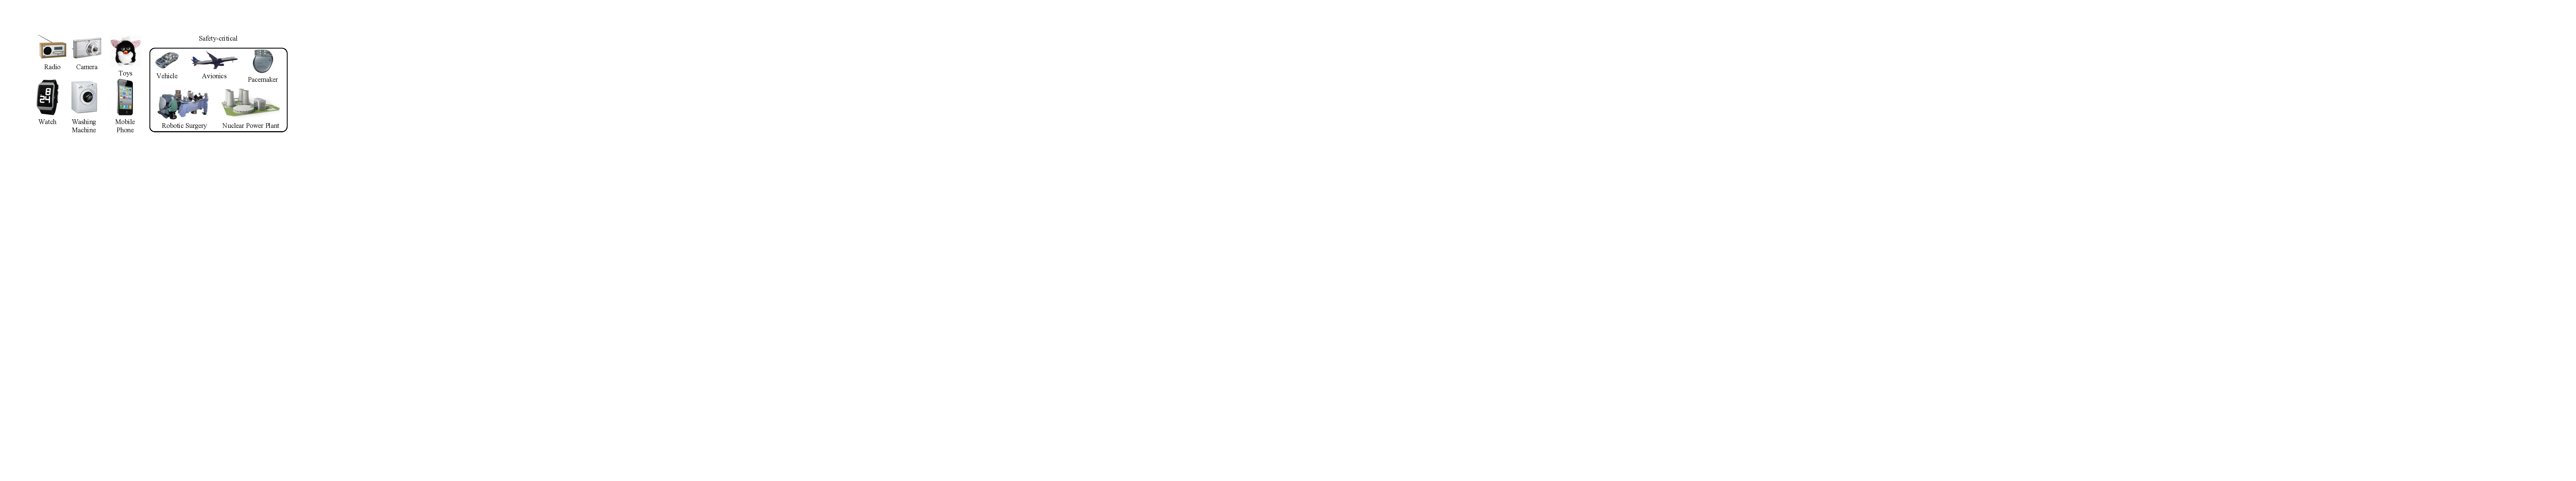
\includegraphics[width=0.9\columnwidth]{embedded_systems}

	\caption{Examples of embedded systems and those with safety-critical concerns.}
	\label{fig:introduction:embedded_systems}
\end{figure}

\subsection{Parallel Programming of Embedded Systems}
\label{sec:introduction:programming}
Programs can be
executed directly by the hardware (bare-metal) or by a
real-time operating system (RTOS)~\cite{pret_merasa_rtos}. 
The bare-metal approach allows all of the system's resources to be used
to execute the program, but code must be included 
to manage the hardware. By contrast, an
RTOS manages the hardware and provides a
consistent environment for developing and executing
programs, thus, enabling code portability across a range of
systems. Hence, the RTOS must be taken into account when analyzing programs. 
C~\cite{programming_languages_c11} is a popular language for 
programming embedded systems with 
support for multi-threading and parallelism 
provided by third-party libraries, compilers, and 
runtime support~\cite{DiazMN12}. Notable 
examples include Pthreads~\cite{multiprocessor_pthreads},
OpenMP~\cite{multiprocessor_openmp}, and
MPI~\cite{multiprocessor_mpi}. 
These multi-threading solutions are inherently
\emph{non-deterministic}~\cite{multiprocessing_problem_threads}
because they allow non-deterministic constructs,
such as race conditions over shared variables in
the case of Pthreads and OpenMP.
The lack of formal semantics for the programming model 
can also lead to ambiguous behaviors. 

Parallel programming is challenging because it requires 
programmers to have specific skills, experience, and 
knowledge to avoid the common parallel programming traps and 
pitfalls~\cite{multiprocessing_debugging_concurrency}. 
For example, parallel accesses to the same shared 
variable will interfere and corrupt the value of the shared variable. 
It is the programmer's responsibility to identify
the regions of code that can interfere, called \emph{critical sections}, 
and ensure that they are executed sequentially at
mutually exclusive times. Hence, programmers need to be 
aware of the data dependencies in their specific program 
and to choose the appropriate solution to manage the dependencies. 
Studies have shown that, without careful tuning~\cite{multithreading_multicore_issues}, 
parallel programs executed on multi-cores can perform 
worse than their sequential counterparts.
The next section describes the use of \emph{synchronous 
languages} as an alternative to creating concurrent programs 
that are deterministic.

\subsection{Synchronous Languages}
\label{sec:introduction:synchronous}

Synchronous languages~\cite{timed_synchronous_survey} 
are based on sound mathematical semantics, which facilitates 
system verification by formal methods~\cite{timed_synchronous_survey} and the
generation of correct-by-construction implementations~\cite{timed_cec,NataleZ12}.
Figure~\ref{fig:introduction:synchronous_moc} depicts a
synchronous program, defined as a set of concurrent threads,
within its physical environment. 
Synchronous programs react continuously to inputs from the environment 
by producing corresponding outputs. Each reaction is triggered by a 
hypothetical (logical) \emph{global clock}. At each global tick, the threads 
in the program sample the environment, perform their computations, and 
emit their results to the environment. When a thread completes its
computation, we say that the thread has completed its
\emph{local tick}. When all threads in the program have
completed their local tick, we say that the program has
completed its \emph{global tick}. Central to synchronous languages 
is the \emph{synchrony hypothesis}~\cite{timed_synchronous_survey}, 
which states that the execution of each reaction is considered to be 
atomic and instantaneous. 
The sampling of inputs avoids the need to use
interrupts which are sources of unpredictable delays that degrade the
system's timing predictability. Concurrent threads
communicate instantaneously with each other (dashed arrows in
Figure~\ref{fig:introduction:synchronous_moc}) due to the
synchrony hypothesis. Once the embedded system is
implemented, the synchrony hypothesis has to be validated.
That is, the worst-case execution time~\cite{wcet_methods_survey} 
of any global tick must not exceed the minimal inter-arrival 
time of the inputs.

\begin{figure}
	\centering
	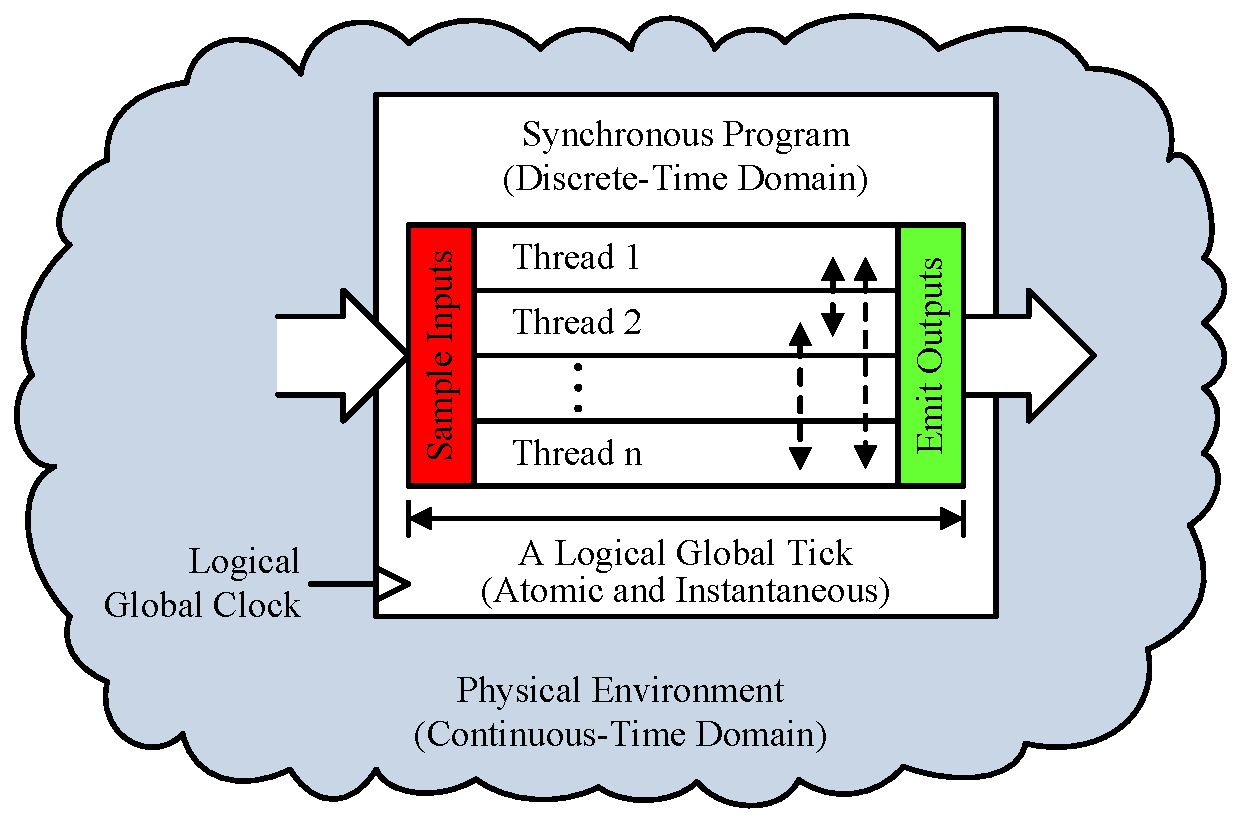
\includegraphics[width=0.8\columnwidth]{synchronous_moc}	

	\caption{Synchronous model of computation.}
	\label{fig:introduction:synchronous_moc}
\end{figure}

\begin{figure}
	\centering

	\subfloat[Esterel]{
		\begin{minipage}[b]{0.4\columnwidth}
			\lstinputlisting[style=full]{./code/Example.strl}
		\end{minipage}
	
		\label{listing:introduction:Example.strl}
	}
	\hfill
	\subfloat[\pretc{}]{
		\begin{minipage}[b]{0.4\columnwidth}
			\lstinputlisting[style=full]{./code/Example.pretc}
		\end{minipage}
		
		\label{listing:introduction:Example.pretc}
	}

	\caption{Examples of synchronous programs.}
\end{figure}

We use the Esterel synchronous language~\cite{timed_esterel}
to illustrate some features of the synchronous paradigm in
Figure~\ref{listing:introduction:Example.strl}. It contains
two threads (starting from lines~\ref{esterel:thread1} and
\ref{esterel:thread2} respectively), scoped between the square brackets
and separated by the parallel operator $\parallel$
(line~\ref{esterel:par}). The parallel operator is
commutative and associative and specifies that both threads
are executed concurrently. The execution of a thread can be
divided over multiple global ticks with the \verb$pause$
statement (e.g., lines~\ref{esterel:pause1},
\ref{esterel:pause2}, and \ref{esterel:pause3}). The
\verb$pause$ statement \emph{pauses} the execution of its enclosing
thread, demarcating the end of the thread's local tick. All
executing threads must pause or terminate to complete the global
tick. Thus, the \verb$pause$ acts as a
synchronization barrier. At the next global tick, the
threads resume from their respective \verb$pause$s. In Esterel, threads
communicate by \emph{emitting} \verb$signal$s and threads can test
for their \emph{presence} or \emph{absence}. For example,
line~\ref{esterel:signal} declares two signals, \verb$A$ and
\verb$B$, that are emitted by the \verb$emit$ statement when
execution reaches lines~\ref{esterel:emit1},
\ref{esterel:emit2}, \ref{esterel:emit3}, and
\ref{esterel:emit4}. An emitted
signal lasts until the global tick ends, becoming absent in
the following global tick unless it is emitted again. Note
that an emitted signal is logically present from the start of the
global tick to ensure that all the threads see the same
signal statuses, even if the \texttt{emit} statement occurs
later in the global tick. In the first global tick, the
first thread emits the signal \verb$A$. At the same time, 
the second thread tests positively for the
presence of \verb$A$ and emits \verb$B$.
Using the \verb$abort$ statement, a body of code can be
\emph{preempted} by the presence of a signal. Preemption provides a
convenient way to model the transitions and states of a
state machine. In the second global tick of the example
program, the second thread enters an \verb$abort$
(line~\ref{esterel:abort}) that preempts its body
(lines~\ref{esterel:abort_body_start}--\ref{esterel:abort_body_end}) 
if \verb$A$ is present.
Because \verb$A$ is not present, the body is not preempted
and \verb$B$ is emitted. Meanwhile, the first thread
terminates because it has reached the end of its body.

Synchronous programs are considerably difficult to 
parallelize~\cite{distributed_reactive_systems_survey,wcrt_esterel_multicores,YuanYR11} 
due to the need to resolve instantaneous thread communication and
associated causality issues. 
At runtime, all potential signal emitters
must be executed before all testers of a signal. 
If this is not possible, then a causality issue arises. 
Thus, concurrency is typically \emph{compiled away} to
produce only sequential code~\cite{timed_cec}. The common approach for
parallelizing synchronous programs is to automatically
parallelize an intermediate representation of the
program~\cite{distributed_reactive_systems_survey,wcrt_esterel_multicores,YuanYR11,multiprocessing_openmp_synchronous}. 
The techniques differ
in the heuristics used to partition the program to achieve
sufficient parallelism. 

Esterel only supports basic data computations and delegates
complex data computations to a host language, for instance C. Consequently, 
C-based synchronous languages have been developed to provide
data handling at the language level. These languages
extend C with a range of synchronous constructs to support
concurrency, preemption, and thread communication. C-based 
synchronous languages appeal to C programmers because the 
learning barrier for synchronous languages is reduced. 
\pretc{}~\cite{pret_pretc} is one such example and
Figure~\ref{listing:introduction:Example.pretc} is the
\pretc{} version of the Esterel example
(Figure~\ref{listing:introduction:Example.strl}). The two
threads (\verb$t0$ and \verb$t1$, defined on
lines~\ref{pretc:t0} and \ref{pretc:t1}) are arguments to
the parallel operator \verb$PAR$ (line~\ref{pretc:par}).
The \verb$EOT$ statement demarcates the end of a thread's
local tick (e.g., lines~\ref{pretc:eot1}, \ref{pretc:eot2},
and \ref{pretc:eot3}). Unlike Esterel, threads in the
\verb$PAR$'s argument are executed in a left-to-right
(static) order. The thread's local tick must be executed
entirely before the next thread can be executed. In the
example program, \verb$t0$ always executes its local tick
before \verb$t1$. In \pretc{}, threads communicate using
globally declared C-variables, not signals. Because
threads are always executed in a static order, the
local ticks always execute in a mutually exclusive manner. 
Hence, threads can safely access shared variables
without needing to use mutual exclusion constructs; all
\pretc{} programs are thread-safe by construction. In
the first global tick of Figure~\ref{listing:introduction:Example.pretc}, 
\verb$t0$ executes first and assigns \verb$1$ to the shared variable
\verb$A$ (line~\ref{pretc:t0_a}). Then, \verb$t1$ executes 
and checks the condition \verb$A==1$, which is \emph{true}, and assigns
\verb$1$ to \verb$B$. \pretc{} does not suffer from causality
issues because global variables are always present and
variables are always accessed sequentially (within a thread and
across threads). \pretc{} supports preemption with the
\verb$abort$ statement but its behavior differs from
Esterel's \verb$abort$. Preemption occurs when the associated
C-condition evaluates to \emph{true}. The condition is
always checked before the \verb$abort$ body is executed. In 
the second global tick of the example program,
\verb$t0$ terminates because it has reached the end of its
body. Then, \verb$t1$ executes and the condition \verb$A==1$
(line~\ref{pretc:abort_cond}) is checked before the
\verb$abort$ body
(lines~\ref{pretc:abort_body_start}--\ref{pretc:abort_body_end}) 
is executed. The condition is \emph{true}, so the body is
preempted. Execution jumps to line~\ref{pretc:abort_body_end} 
and \verb$t1$ terminates. 

Other C-based synchronous languages exist, such as \synchronousc{}~\cite{timed_synccharts_c_proposal}
and Esterel~C Language~\cite{timed_ecl},
and are reviewed in Section~\ref{sec:literature}. 
However, these languages are not designed to take advantage 
of parallel execution. This paper focuses on developing a C-based,
synchronous language for writing parallel programs that
perform well on multi-core processors and are amenable to 
static timing analysis. 

\subsection{Programming Safety-Critical Embedded Systems}
\label{sec:introduction:programming_safety}
Safety-critical embedded systems need to be 
certified against stringent safety standards, such as 
DO-178B~\cite{DO-178B} or IEC 61508~\cite{IEC61508}, before
they can be deployed and used in the field.
Although the C language is popular for programming safety-critical embedded systems, 
its semantics~\cite{programming_languages_c11} includes unspecified 
and undefined behaviors~\cite{safety_critical_coding_traps_pitfalls}. Strict 
coding guidelines~\cite{safety_critical_coding_misrac_standard,safety_critical_coding_power_10,safety_critical_coding_jpl} 
are typically used by safety-critical programmers to help write well 
defined programs that are deterministic, understandable, maintainable, 
and easier to debug~\cite{safety_critical_coding_structure,safety_critical_coding_misrac_overview}. 
The coding guidelines can be grouped into three main areas: 
\begin{description}
	\item[Code clarity] These guidelines suggest a style for writing programs
		  free of ambiguous statements and to structure code for readability. 
		  For example, the use of braces to clarify the nesting of \verb$if$--\verb$else$ statements
		  or the forbidding of \texttt{goto} statements.
		  Code clarity helps static analyzers parse the program and 
		  attain greater analysis precision.
		
	\item[Defensive programming] These guidelines help minimize the use of 
		  unspecified and undefined behaviors, which contribute to
		  non-determinism. For example, the C semantics does not specify 
		  the evaluation order of multiple expressions, e.g.,
		  in function arguments. Thus, function 
		  arguments with side-effects may evaluate to different values 
		  depending on the evaluation order used by the implementation.
		  To ensure deterministic evaluation~\cite{programming_languages_cholera}, 
		  expressions must not contain any assignment operators, e.g., ``\texttt{=}'', 
		  ``\texttt{+=}'', or ``\texttt{++}''. Furthermore, 
		  the sequencing operator ``\texttt{,}'' must not be 
		  used in expressions.
		
	\item[Runtime reliability] These guidelines help prevent runtime errors 
		  from occurring, even when the program is written correctly. 
		  For example, a runtime error occurs when a program requests for 
		  more memory than is available in the implemented system. To prevent
		  it, memory is always allocated statically at the start of the program.
		  Static verification tools, such as Parasoft~\cite{parasoft}, 
		  Polyspace~\cite{polyspace}, and Parallel Lint~\cite{parallel_lint}, 
		  can be used to identify possible runtime defects.
\end{description}


\subsection{Contributions}
We propose the ForeC parallel programming language for simplifying the
deterministic parallel programming of embedded multi-core systems. 
Execution platforms have evolved from 
single-cores to multi-cores. Hence, all the synchronous languages 
designed for the single-core era must be reinvented to address the 
multi-core challenges. To this end, ForeC is a C-based 
synchronous language designed specifically
for the programming of multi-cores. ForeC brings together the formal 
deterministic semantics of synchronous languages and the benefits of 
C's control and data structures. A key innovation is ForeC's shared 
variable semantics that provides thread isolation and deterministic 
thread communication. Moreover, many forms of parallel patterns
can be expressed in ForeC. We show that ForeC programs are reactive and 
deterministic by construction. ForeC can be compiled for direct execution
on embedded multi-cores or for execution by an OS on desktop multi-cores.
Through benchmarking, we demonstrate that ForeC can achieve better parallel 
performance than Esterel and OpenMP, while also being amenable to static 
timing analysis.

\subsection{Paper Organization}
This paper is organized as follows.
Section~\ref{sec:literature} provides a detailed literature review of
parallel and synchronous programming languages.
Section~\ref{sec:architecture_multicore} describes the multi-core architecture
considered by this paper.
Section~\ref{sec:forec} introduces the ForeC language,
defines the formal semantics, and provides
proofs for determinism and reactivity.
Section~\ref{sec:forec_compiling} describes our compilation
approach for generating code that delivers good parallel performance
and that is amenable to static timing analysis.
Section~\ref{sec:forec_benchmarking} presents benchmarking results
for ForeC's performance on multi-cores and the time predictability
of its execution.
Section~\ref{sec:conclusion} concludes the paper.


%\section{Related Work}
\section{Related Work}
\label{sec:literature}
Designing embedded systems that are time-predictable remains 
an open challenge~\cite{AxerEFGGGJMRRSHWY14}. Moreover, the 
growth of embedded multi-cores is pushing more
programmers to be parallel programming experts. 
Table~\ref{table:literature:mutual_exclusion} 
highlights different approaches for enforcing \emph{mutual
exclusion} on shared variables, usually by interleaving 
the parallel accesses to enforce a sequence of accesses to 
the \emph{critical sections}.
As argued by Lee~\cite{multiprocessing_problem_threads}, 
the adoption of parallelism in sequential languages, like C~\cite{programming_languages_c11}, 
discards important properties, such as determinism, predictability,
and understandability. Thus, programmers spend large 
amounts of time taming the non-determinism in their parallel 
programs~\cite{multiprocessing_debugging_concurrency_study}. 
Instruction reordering is regularly employed by compilers 
and processor cores to maximize execution parallelism, but this
can cause wrong values for shared variables to be observed.
C provides the programmer with memory fences to enforce a partial 
ordering on variable accesses between threads: all side-effects of 
a \emph{releasing} thread are committed before the \emph{acquiring} 
thread leaves the fence. To help tame non-determinism, runtime environments 
that enforce deterministic thread scheduling and memory
accesses can be used. Such runtime environments have been 
developed for Linux processes (DPG~\cite{multiprocessing_dos}), 
Pthreads (Grace~\cite{multiprocessing_grace}, 
Kendo~\cite{multiprocessing_kendo}, CoreDet~\cite{multiprocessing_coredet}, 
and Dthreads~\cite{multiprocessing_dthreads}), OpenMP 
(DOMP~\cite{multiprocessing_domp}), and 
MPI (DetMP~\cite{multiprocessing_detmp}).
For DPG, Kendo, CoreDet, and Dthreads, all thread interactions
are mapped deterministically onto a logical timeline (which
progresses independently of physical time). Program execution
is divided into alternating parallel and serial phases, similar to
the Bulk Synchronous Parallel (BSP)~\cite{Valiant90} programming model. In 
the parallel phase, threads execute in parallel until they all reach
one of the following synchronization points: a lock, memory access, 
or statically defined number of executed instructions. 
Then, in the serial phase, threads take turns to resolve their memory 
accesses or lock acquisitions. Threads in CoreDet and Dthreads 
also maintain their own version of the shared memory state, which
is resynchronized in every serial phase. This concept 
is used and formally defined in concurrent revisions~\cite{BurckhardtL11}. 
DOMP and Grace differ in that the resynchronization only 
occurs when threads reach a synchronization construct.
However, understanding the program's behavior at compile time 
remains difficult because the determinism is only enforced at 
runtime. Thus, if the program is modified, e.g., to fix a 
bug, then a vastly different runtime behavior is possible.  
An alternative is to directly extend and 
modify the C language with deterministic parallelism, such as
SharC~\cite{multiprocessing_data_race_detection}, 
\textsc{CAT}~\cite{multiprocessing_cat}, 
SHIM~\cite{multiprocessing_shim_scheduling}, 
$\Sigma$C~\cite{multiprocessing_sigmac}, and
ForkLight~\cite{multiprocessing_forklight}. These solutions 
allow the asynchronous forking and synchronized joining 
of threads, but lack a convenient mechanism for preempting 
groups of threads. However, their timing predictability 
has not been demonstrated, which is required for programming 
safety-critical embedded systems.

\begin{table}
	\def\arraystretch{1.3}

	\tbl{Existing solutions for avoiding race conditions.\label{table:literature:mutual_exclusion}} {
		\begin{tabular}{| p{\textwidth} |}
			\hline
			\textbf{Programming Constructs:}
			These are constructs written in the host language to provide mechanisms for the 
			programmer to achieve mutual exclusion. Examples include: locks, monitors, memory fences,
			transactional memory, message passing, and parallel data structures. Using these 
			constructs correctly can be tedious and error prone for large programs and may lead to other 
			errors~\cite{multiprocessing_problem_threads,multiprocessing_debugging_concurrency,multiprocessing_debugging_concurrency_study}, 
			e.g., deadlocks, starvation, or priority inversion.									\\ \hline
		
			\textbf{Language Semantics:}
			The language semantics can have a memory model that defines how threads interact 
			through memory, what value a read can return, and when the value of a write becomes 
			visible to other threads. Although the memory model can prevent race conditions, it 
			may only be suitable for a few types of applications. Examples include: synchronous 
			languages~\cite{timed_synchronous_survey}, \pretc{}~\cite{pret_pretc}, Synchronous 
			C~\cite{timed_synccharts_c_proposal}, SharC~\cite{multiprocessing_sharc}, 
			Deterministic Parallel Java~\cite{multiprocessing_dpj}, SHIM~\cite{multiprocessing_shim_cell}, 
			$\Sigma$C~\cite{multiprocessing_sigmac}, concurrent revisions~\cite{BurckhardtL11}, and 
			Reactive Shared Variables~\cite{timed_reactivec_shared_variables}. 					\\ \hline
		
			\textbf{Static Analysis:}
			A compiler or static analyzer can identify and alert the programmer regarding the race 
			conditions in their program (e.g., Parallel Lint~\cite{parallel_lint}) and may try 
			to resolve them by serializing the parallel accesses for the programmer 
			(e.g., Sequentially Constructive Concurrency~\cite{timed_seq_concurrency}). However, 
			programmer guidance is needed for race conditions that cannot be resolved.			\\ \hline
		
			\textbf{Runtime Support:}
			Programs are executed on a runtime layer that dynamically enforces deterministic 
			execution and memory accesses. Examples include: dOS~\cite{multiprocessing_dos},
			Grace~\cite{multiprocessing_grace}, Kendo~\cite{multiprocessing_kendo}, 
			CoreDet~\cite{multiprocessing_coredet}, Dthreads~\cite{multiprocessing_dthreads}, 
			DOMP~\cite{multiprocessing_domp}, and DetMP~\cite{multiprocessing_detmp}. However, 
			understanding the program's behavior at compile time remains difficult because the 
			determinism is only enforced at runtime.											\\ \hline
		
			\textbf{Hardware Support:}
			Parallel accesses can be automatically detected and resolved by the hardware, preventing
			race conditions from happening. Examples include: Ultracomputer's combine hardware~\cite{Schwartz80} 
			and certain shared bus arbitration (e.g., round-robin, TDMA, and priority). However, the 
			timing of the parallel accesses affects how they are interleaved.					\\
			\hline
		\end{tabular}
	}
\end{table}

The classic synchronous languages
are Esterel~\cite{timed_esterel}, Lustre~\cite{timed_lustre}, 
Signal~\cite{timed_signal}, and the recent extension based 
on functional programming such as Lucid Synchrone~\cite{ColacoP03}, 
and are well suited to the modeling 
of control-dominated systems~\cite{CaspiM05} and
safety-critical systems~\cite{timed_synchronous_survey}. 
To increase their uptake with embedded programmers, 
C-based synchronous languages have
been developed, such as Reactive Shared Variables~\cite{timed_reactivec_shared_variables}, 
Esterel C Language (ECL)~\cite{timed_ecl}, \pretc{}~\cite{pret_pretc} and 
\synchronousc{} (SC)~\cite{timed_synccharts_c_proposal,timed_seq_concurrency}. 
The inherent sequential execution semantics of SC, 
Reactive Shared Variables, and \pretc{} renders them 
unsuitable for multi-core execution.
Moreover, concurrency in synchronous languages is a logical concept 
to help the programmer handle concurrent inputs, rather
than a specification for parallel execution.
Thus, compilers typically generate only sequential 
code~\cite{timed_cec,timed_compiling_esterel}, 
although some generate concurrent 
tasks~\cite{CaspiSST08,NataleGZS10,PagettiFBCL11,NataleZ12}
for execution on single-cores. Yuan et al.~\cite{YuanYR11,Yuan13} 
offer a static and dynamic scheduling approach for Esterel
on multi-cores. For the static approach, threads are statically
load-balanced across the cores and signal statuses are resolved 
at runtime. For the dynamic approach, threads that need to be
scheduled for execution are inserted into a custom hardware 
queue accessible to all cores. The dynamic approach has been shown 
to provide better average-case performance compared to the static 
approach~\cite{Yuan13}. This is because the static approach 
uses worst-case execution times to load-balance the threads, even 
though the actual execution times may be shorter.

The common approach for parallelizing synchronous programs is to 
parallelize an intermediate representation of the sequentialized 
code~\cite{distributed_reactive_systems_survey,wcrt_esterel_multicores,YuanYR11,distributed_synchronous_dependency_driven,distributed_reactive_systems_automatic,timed_esterel_distribution_emperor,timed_multiclock_multithreaded}.
Multi-threaded OpenMP programs can be generated from the Synchronous 
Guarded Actions intermediate format~\cite{multiprocessing_openmp_synchronous}.
The techniques differ in the heuristics used to partition
and distribute the program to achieve sufficient parallelism.
The Synchronized Distributed Executive 
(SynDEx)~\cite{distributed_synchronous_semantics_preserving} 
approach considers the cost of communication when distributing
code to each processing element. When distributing a synchronous 
program, some desynchronization~\cite{BenvenisteCG00,GiraultNP06,distributed_synchronous_desynchronize_modes} 
is needed among the concurrent threads. That is, the concurrent 
threads execute at their own pace, but sufficient inter-thread 
communication is used to preserve the original synchronous 
semantics. The use of \emph{futures} has been proposed as a method for 
desynchronizing long computations in 
Lustre~\cite{multiprocessing_lustre_futures}. A \emph{future}
is a proxy for a result that is initially unknown but becomes 
known at a later time and can be computed in parallel with 
other computations. 

Once a synchronous program is implemented, it is necessary
to validate the synchrony hypothesis. 
That is, the worst-case execution time~\cite{Wilhelm14,wcet_methods_survey} 
(WCET) of any global tick must not exceed the minimal 
inter-arrival time of the inputs. This is known as 
worst-case reaction time (WCRT) 
analysis~\cite{wcrt_concurrent_reactive,wcrt_algebra_interfaces} and
various techniques have been developed for 
single-cores~\cite{wcrt_algebra_interfaces,JuHRC12,WangRA13,RaymondMPC13,wcrt_taxys,AndalamRG11,wcrt_concurrent_reactive,KuoSR11} 
and multi-cores~\cite{wcrt_esterel_multicores,YipRAG13}.


%=========================================================================

\subsection{Discussion}
This section has presented a snapshot of the current efforts
in the programming of time-predictable CPSs.
Many of the attempts at providing deterministic
parallelism have used concepts found in
synchronous languages. C-based synchronous languages
have much to offer to embedded programmers in terms of
deterministic concurrency and formally verifiable
implementations, but lack support for parallel execution.
This paper tackles the lack of a C-based synchronous
parallel programming language that offers \emph{both} 
time-predictability and good parallel execution performance.


%\section{Architecture of the Multicore Processor}
\section{Multi-Core Architecture}
\label{sec:architecture_multicore}
Embedded systems continue to explode in
complexity and functionality~\cite{sld_complexity}. To meet
the size, weight, and power (SWaP) concerns, the advent of
affordable embedded multi-core
processors~\cite{multithreading_multicore,multithreading_multicore_parallelism} 
offer designers the opportunity to achieve better performance 
than single-core processors.
Figure~\ref{fig:introduction:multi_core} illustrates the
architecture of a general-purpose multi-core. In pursuit of
increasing average-case performance, the cores typically
include speculative 
features~\cite{multithreading_cpu_overview} such as
out-of-order execution, branch prediction, data forwarding,
superscalar execution, and 
on-chip caches. However, such optimizations can cause
\emph{timing anomalies}~\cite{LundqvistS99} where a local
worst-case execution time does not lead to the program's
worst-case execution time. Thus, speculation leads to the
degradation of time-predictability and is undesirable for embedded systems.
The PREcision Timed (PRET) machine~\cite{pret_pret,pret_repeatable_timing} and
PRedictability Of Multi-Processor Timing
(PROMPT)~\cite{multithreading_designing_predictable_considerations,KastnerSPCGHF12} 
design philosophies aim to tackle this issue by advocating the
design of \emph{predictable hardware architectures}, while
not sacrificing performance. In particular, the architecture
should provide \emph{timing isolation} between the cores,
i.e., the actions of the cores must not influence each
other's timing behavior. The architecture should be
\emph{timing compositional}, i.e., with repeatable timing behavior
and free of timing anomalies. The following are examples
of unpredictable hardware features with possible predictable
alternatives~\cite{wcet_future_architectures,multithreading_designing_automotive,multithreading_predictable_multiprocessor}:
\begin{itemize}
	\item \emph{Replace caches with fast software managed memories, called scratchpads~\cite{memory_scratchpad_predictable}.}
		  The selection of data and instructions to be allocated to a scratchpad is determined entirely at 
		  compile time~\cite{memory_scratchpad_known_size,memory_scratchpad_concurrent_allocation,KimBCS14,PrakashP13a,memory_scratchpad_unknown_size}. 
		  In the static allocation scheme, the contents of the scratchpad cannot be changed at runtime. In the
		  dynamic allocation scheme, the contents of the scratchpad can be changed at runtime by using compile time decisions.
		  Importantly, the replacement policy of scratchpads is controllable, whereas with caches the replacement policy is controlled by 
		  the hardware, sometimes with unpredictable behaviors (e.g., with the PLRU policy).
		  The memory address spaces of scratchpads and global memory are mutually exclusive. 
		
	\item \emph{Replace out-of-order execution with better code generation from the compiler~\cite{wcet_aware_framework,SchranzhoferPCTC11,memory_multicore_code_positioning,memory_shared_cache_aware_wcrt,pret_merasa}.}
		  A processor's ability to reorder a group of instructions is limited by the size of
		  its instruction buffer. The compiler does not have this limitation because
		  it has access to the entire program and can make better judgments when reordering
		  instructions. However, it may not have the runtime execution information which may affect the performance.

	\item \emph{Deactivate high-performance bus features, such as burst transfers or pipelining, 
		  and use fair time-sharing arbitration policies, such as round-robin or time
		  division multiple access (TDMA)~\cite{memory_tdma_priority_division}.}
		  The round-robin policy cycles through a static list of 
		  cores, granting them access to the bus. If the granted core does not need the bus, then
		  the grant is given to the next core on the list. The TDMA policy cycles through
		  a static list of cores, granting them access for a fixed amount of time 
		  (a time slot), whether the core needs it or not. 
		  If the granted core does not need the bus, then some 
		  policies~\cite{memory_tdma_priority_division,memory_buses,memory_tdma_lottery,memory_arbitration_performance,HamannE05} will 
		  grant the slot to the other cores in a round-robin manner, thus 
		  improving the throughput. Fairness of the arbitration is important to ensure 
		  that all accesses complete within a bounded length of time.
\end{itemize}
Embedded systems designed using the PRET~\cite{pret_repeatable_timing} or PROMPT~\cite{KastnerSPCGHF12}
philosophies are simpler to understand, model, and analyze.
Many predictable single-core processors have been proposed,
such as the %Multiple Active Context System 
MACS~\cite{pret_macs}, 
%Microprogrammed Coarse Grained Reconfigurable Processor 
MCGREP~\cite{pret_mcgrep}, Patmos~\cite{pret_patmos}, %PRET ARM
PTARM~\cite{LiuRBZL12}, and FlexPRET~\cite{ZimmerBSL14} processors.
%Multi-Core Execution of Hard Real-Time Applications Supporting Analysability 
MERASA~\cite{pret_merasa} is a 
predictable multi-core processor that supports hard and non-real-time
threads. Hard real-time threads access scratchpads for predictability, 
while non-real-time threads access caches for performance. An analyzable
memory controller is used to arbitrate shared bus accesses from the cores.
For Java programs, there is the %Java Optimized Processor 
JOP~\cite{pret_java_architecture} processor and its multi-core 
variant~\cite{pret_jop_cmp_scalability} that uses scratchpads and 
a shared TDMA bus.

\begin{figure}
	\centering
	
	\begin{minipage}[t]{0.45\columnwidth}
		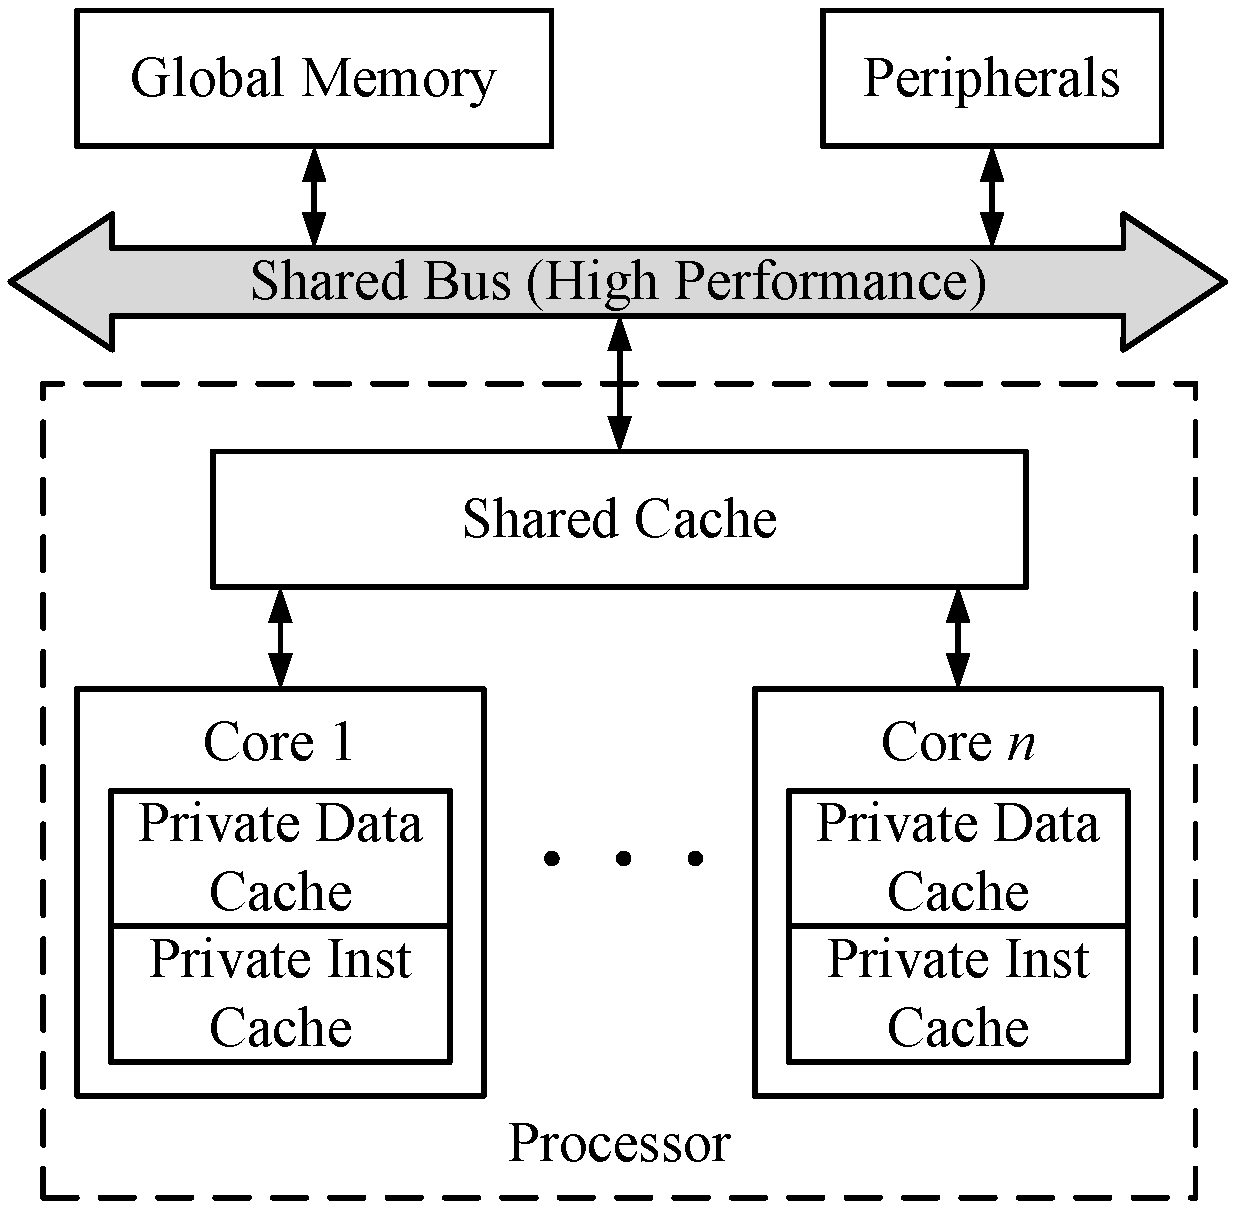
\includegraphics[width=\textwidth]{multi_core}
		\caption{General multi-core architecture.}
		\label{fig:introduction:multi_core}
	\end{minipage}
	\hfill
	\begin{minipage}[t]{0.45\columnwidth}
		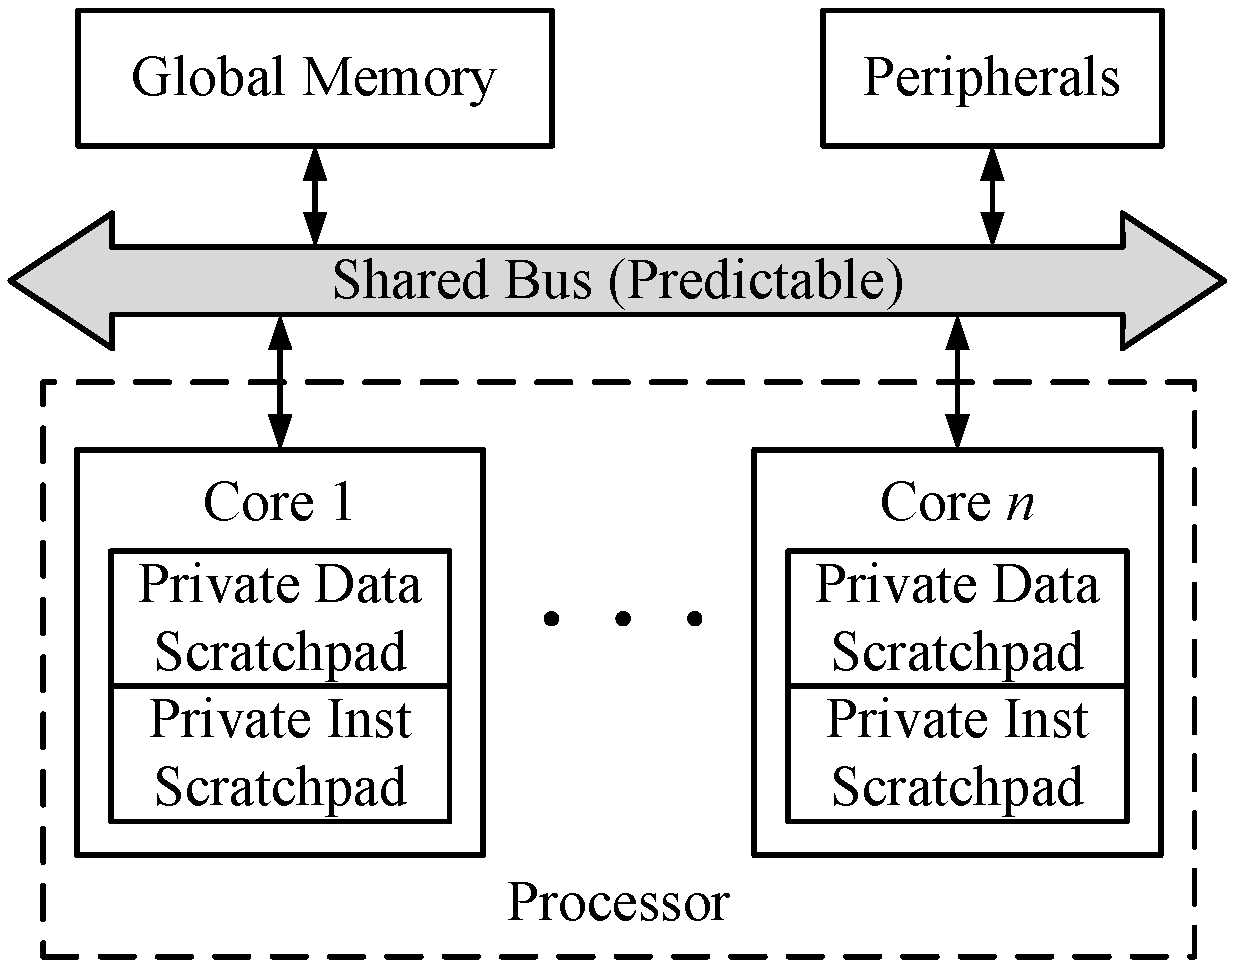
\includegraphics[width=\columnwidth]{multi_core_embedded}
		\caption{Example of a predictable multi-core embedded architecture.}
		\label{fig:introduction:multi_core_embedded}
	\end{minipage}
\end{figure}

The execution of synchronous programs can be accelerated by
\emph{reactive processors}~\cite{SalcicBB02,LiH12}, which
have hardware support for signal resolution, concurrency,
preemptions, and global tick synchronization. A key feature
is their ability to execute programs in a time predictable
manner. Single-core multi-threaded reactive processors
include %Kiel Esterel Processor 
KEP~\cite{LiH12} and %Simultaneous multiThreaded
%Auckland Reactive Processor 
STARPro~\cite{YuanAYRS09}.
Reactive multi-processors include %Embedded
%MultiProcessor supporting Esterel Reactive OpeRations
EMPEROR~\cite{DayaratneRS06} and %HybriD Reactive Architecture 
HiDRA~\cite{SalcicHRB06}. However, these
reactive processors and associated compilers do not support
the execution of host functions written in a host language,
such as C. As a compromise between efficiency and host 
language support, a general purpose processor can be
patched with a reactive functional unit to accelerate the
execution of synchronous constructs. The %Auckland Reactive PRET 
ARPRET~\cite{AndalamRG10} processor is a
patched Xilinx MicroBlaze~\cite{microblaze} processor tailored for executing \pretc{}. 
Java-based reactive single-core processors include %Reactive JOP 
RJOP~\cite{NadeemBS11} and %Tandem Processor JOP 
TP-JOP~\cite{LiMS14}.  %GALS Heterogeneous Multiprocessor 
GALS-HMP~\cite{SalcicM13} is a Java-based reactive multi-processor.

\subsection{Predictable Embedded Multi-Core Architecture}
\label{sec:introduction:pret:multicore}
The architecture of the predictable multi-core used in this 
paper is representative of existing designs.
It is a homogeneous multi-core 
processor~\cite{multithreading_designing_predictable_considerations,pret_java_architecture}
that we have designed using identical Xilinx MicroBlaze~\cite{microblaze} cores, 
illustrated in Figure~\ref{fig:introduction:multi_core_embedded}. 
Each MicroBlaze core has a three-stage, in-order, timing anomaly-free pipeline 
connected to private data and instruction scratchpads.
The scratchpads are statically allocated and loaded at compile time. A shared 
bus with TDMA arbitration connects 
the cores to shared resources, such as global memory and peripherals. Due to 
the resource constraints of existing FPGA devices, we developed a multi-core MicroBlaze
simulator for benchmarking 
purposes. We extended an existing MicroBlaze simulator~\cite{mb_simulator} 
significantly to support cycle-accurate simulation, an arbitrary number of cores, 
and a shared bus with TDMA arbitration.


%\section{The ForeC Language}
\section{The ForeC Language}
\label{sec:forec}
Execution platforms have evolved from single-cores to multi-cores. 
Hence, all the synchronous languages designed earlier (e.g., 
Esterel~\cite{timed_esterel}, Lustre~\cite{timed_lustre},  
Signal~\cite{timed_signal}, Esterel C Language~\cite{timed_ecl}, 
Reactive Shared Variables~\cite{timed_reactivec_shared_variables}, 
and \pretc{}~\cite{pret_pretc}) must be remodeled to 
address the challenges raised by multi-cores. Over 30 years of
synchronous programming languages have demonstrated that they
are very well suited to the design of safety-critical real-time
systems~\cite{BriereRPC95,SouyrisPHJBH05}. Moreover, the ideal modeling of 
time brought by the synchrony hypothesis makes them good 
candidates for PRET programming. This motivates our proposed
ForeC language that is dedicated to the programming of multi-cores. 
ForeC inherits the benefits of synchrony, such as determinism
and reactivity, along with the benefits and power of the C language, 
such as control and data structures. This is unlike conventional
synchronous languages, which treat C as an external host language.
A key goal of ForeC is in providing deterministic shared variable
semantics that is agnostic to scheduling. This goal
is essential for the reasoning and debugging of parallel
programs. This section presents ForeC with a 
UAV running example. The formal
semantics of ForeC is then detailed and important proofs
concerning program reactivity and 
determinism~\cite{Maraninchi92,Tardieu07} are provided.

\subsection{Overview and Syntax}
\label{sec:forec:overview}
ForeC is a synchronous language that extends a
safety-critical subset of C~\cite{programming_languages_clight,programming_languages_cyclone} 
(see Section~\ref{sec:introduction:programming_safety}) with a
minimal set of synchronous constructs. We briefly describe the 
statements, type specifiers, and type qualifiers allowed in the C subset:
\begin{description}
	\item[C statements (\emph{c\_st})]
		  Expressions in a statement can only be constants, variables, pointers, and 
		  arrays that are composed with the logical, bitwise, relational, and 
		  arithmetic operators of C. 
		  Although the use of pointers and arrays is allowed, they can make static
		  dataflow analysis difficult~\cite{BussBSE10} because of pointer aliasing. 
		  Thus, we assume that pointers are never reassigned to 
		  point to other variables.
		  All C control statements, except \texttt{goto}, can be used. These are the selection statements 
		  (\texttt{if}--\texttt{else} and \texttt{switch}) and loop statements (\texttt{while}, 
		  \texttt{do}--\texttt{while}, and \texttt{for}).

	\item[C type specifiers] All the C primitives can be used, e.g., \texttt{char}, 
		  \texttt{int}, and \texttt{double}. Custom data types can be defined using
		  \texttt{struct}, \texttt{union}, and \texttt{enum}.

	\item[C type qualifiers (\emph{c\_tq})] All the C \texttt{const}, 
		  \texttt{volatile}, and \texttt{restrict} qualifiers can be used.
		  
	\item[C storage class specifiers] The C \texttt{typedef},
		  \texttt{extern}, \texttt{static}, \texttt{auto}, and \texttt{register} specifiers can be
		  used.
\end{description}

Figure~\ref{fig:forec:syntax} gives
the extended syntax of ForeC and Table~\ref{table:forec:semantics}
summarizes the informal semantics. A statement (\emph{st}) in ForeC
can be a traditional C statement (\emph{c\_st}), or a barrier (\verb$pause$), 
fork/join (\verb$par$), or preemption (\verb$abort$) statement. Using 
the sequence operator (~;~), a statement in ForeC can be an 
arbitrary composition of other statements. Like C, extra
properties can be specified for variables using type
qualifiers. A type qualifier (\emph{tq}) in ForeC is a
traditional C type qualifier (\emph{c\_tq}), an environment
interface (\verb$input$ and \verb$output$), or a
shared variable amongst threads (\verb$shared$). The \verb$input$, 
\verb$output$, and \verb$shared$ type qualifiers precede the 
C type qualifiers in variable declarations. 

\begin{figure}
	\centering
	\begin{tabular}{| l r l |}
		\hline
		\textbf{Statements:}		& \emph{st} & ::= \emph{c\_st} \textbar{} \verb$pause$ \textbar{} \verb$par($\emph{st},~\emph{st}\verb$)$	\\
									&			& ~~~~~\textbar{} \verb$weak$?~\verb$abort$~\emph{st}~\verb$when immediate$?~(\expression{})	\\
									&			& ~~~~~\textbar{} \emph{st}; \emph{st}															\\
									&			&																								\\
		\textbf{Type Qualifiers:}	& \emph{tq}	& ::= \emph{c\_tq} \textbar{} \verb$input$ \textbar{} \verb$output$ \textbar{} \verb$shared$	\\
		\hline
	\end{tabular}
	
	\caption{Syntactic extensions to C.}
	\label{fig:forec:syntax}
\end{figure}

\begin{table}
	\def\arraystretch{1.3}
	
	\tbl{ForeC constructs and their semantics.\label{table:forec:semantics}}{
		\begin{tabular}{| p{\textwidth} |}
			\hline
			\texttt{input}:
				Type qualifier to declare an input, the value of which is updated 
				by the environment at the start of every global tick.						\\ \hline
			\texttt{output}:
				Type qualifier to declare an output, the value of which is emitted 
				to the environment at the end of every global tick.							\\ \hline
			\texttt{shared}:
				Type qualifier to declare a shared variable, which can be accessed by 
				multiple threads.															\\ \hline
			\texttt{pause}:
				Pauses the executing thread until the next global tick.						\\ \hline
			\texttt{par}(\emph{st},~\emph{st}):
				Forks two statements \emph{st} as parallel threads. The 
				\texttt{par} terminates when both threads terminate (join back).			\\ \hline
			\texttt{weak}?~\texttt{abort}~\emph{st}~\texttt{when immediate}?~(\expression{}):
				Preempts its body \emph{st} when the expression \expression{} evaluates to 
				a non-zero value. The optional \texttt{weak} and \texttt{immediate} keywords 
				modify its temporal behavior.												\\
			\hline
		\end{tabular}
	}
\end{table}

\begin{figure}
	\centering
	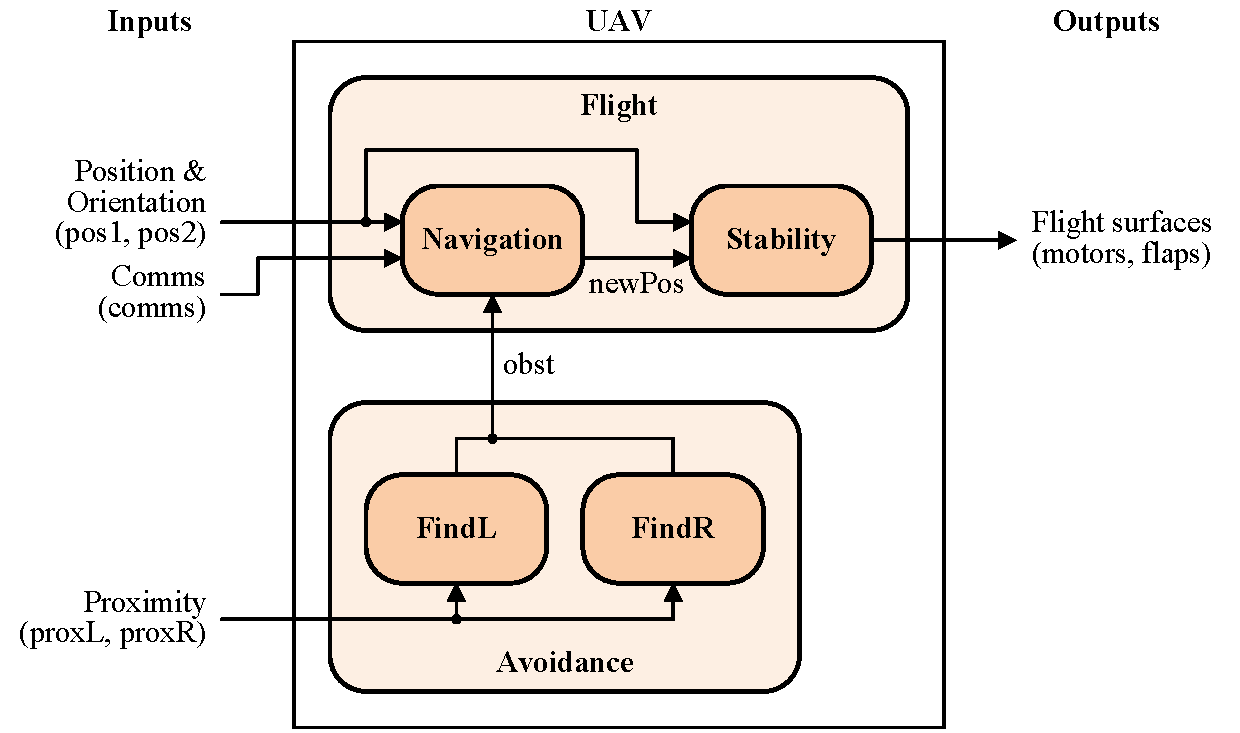
\includegraphics[width=\columnwidth]{images/uav_forec.pdf}

	\caption{Tasks of the UAV.}
	\label{fig:forec:uav_forec}
\end{figure}

As a running example to illustrate the ForeC language, we describe the
design of an unmanned aerial vehicle (UAV) inspired by the
Paparazzi project~\cite{benchmark_papabench}. A UAV is a
remotely controlled aerial vehicle commonly used in
surveillance operations. Figure~\ref{fig:forec:uav_forec} 
presents the functionality of the UAV as a block diagram of tasks. 
The UAV consists of two parallel tasks called \verb$Flight$
and \verb$Avoidance$. The \verb$Flight$ task consists of
two parallel tasks called \verb$Navigation$ and \verb$Stability$.
The \verb$Navigation$ task localizes the UAV with on-board
sensors, updates the flight path, and sends the desired
position to the \verb$Stability$ task. The \verb$Stability$
task controls the flight surfaces to ensure stable flight to
the desired position. The \verb$Avoidance$ task consists of 
two parallel tasks called \verb$FindL$ and \verb$FindR$. 
These tasks use on-board sensors to detect obstacles around 
the UAV and sends collision avoidance data to the 
\verb$Navigation$ task. 

Figure~\ref{fig:forec:uav} is a ForeC implementation of the 
UAV example given in Figure~\ref{fig:forec:uav_forec}.
Figure~\ref{fig:forec:uav_timing1} is a possible execution 
trace of Figure~\ref{fig:forec:uav} to help illustrate the 
execution of ForeC programs. Sections~\ref{sec:introduction:synchronous}
described the execution behavior of synchronous programs. 
To recap, the threads of a synchronous program execute in 
lock-step to the ticking of a \emph{global clock}. In each 
global tick, the threads sample the environment, perform their
computations, and emit their results to the environment.
When a thread completes its computation, we say that it 
has completed its \emph{local tick}. When all the threads complete
their local ticks, we say that the program has completed 
its \emph{global tick}. In Figure~\ref{fig:forec:uav_timing1}, 
the first three global ticks are demarcated along 
the left-hand side. 

\begin{figure}
	\centering
	\begin{minipage}[t]{0.75\columnwidth}
		\lstinputlisting[style=full]{./code/forec/informal/uav.forec}
	\end{minipage}
	\caption{Example ForeC program for the UAV running example.}
	\label{fig:forec:uav}
\end{figure}

\begin{figure}
	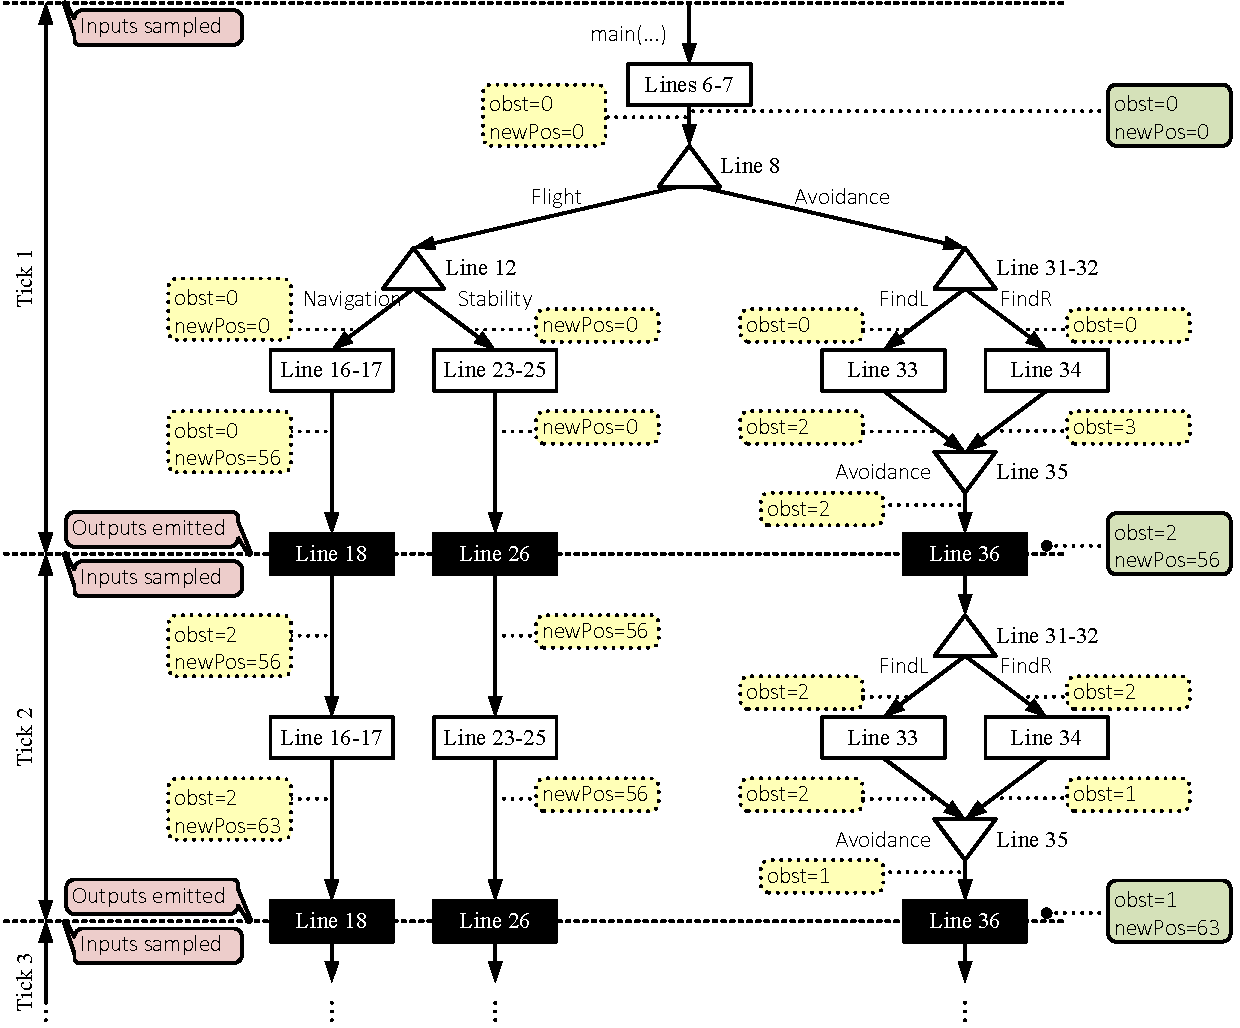
\includegraphics[width=\columnwidth]{images/uav_timing1.pdf}
	\caption{Possible execution trace for Figure~\ref{fig:forec:uav}.}
	\label{fig:forec:uav_timing1}
\end{figure}

In Figure~\ref{fig:forec:uav}, the UAV program starts with 
the inclusion of a C header file (line~\ref{code:forec:uav_header}) 
for the functions used in the 
program and the global variable declarations 
(lines~\ref{code:forec:uav_inputs}--\ref{code:forec:uav_outputs}) to 
interface with the environment. Line~\ref{code:forec:uav_inputs}
declares inputs to capture sensor readings. Inputs
are read-only and their values are updated by the
environment at the start of every global tick. 
Line~\ref{code:forec:uav_outputs} declares outputs
for the actuation commands for the flight motors and
surfaces. Outputs emit their values to the
environment at the end of every global tick. Inputs and
outputs can only be declared in the program's
global scope. The left-hand side of Figure~\ref{fig:forec:uav_timing1}
shows the sampling of inputs and emission of outputs 
at the start and end of each global tick, respectively.

Like traditional C programs, the function \verb$main$ 
(line~\ref{code:forec:uav_main}) is the program's main 
entry point and serves as the initial
thread of execution. Lines~\ref{code:forec:uav_obst}--\ref{code:forec:uav_newpos}
declare variables that can be shared amongst 
threads (see Section~\ref{sec:forec:shared_variables}).
In Figure~\ref{fig:forec:uav_timing1}, the states of 
the shared variables are given inside solid round
boxes at specific points in the execution trace.
Line~\ref{code:forec:uav_obst} declares a shared
variable \verb$obst$ to store the distance and angle 
of the closest obstacle as an encoded integer.
Line~\ref{code:forec:uav_newpos} declares a shared variable
\verb$newPos$ to store the UAV's desired position. 

On line~\ref{code:forec:uav_par1}, the \verb$par$ statement
forks the \verb$Flight$ (line~\ref{code:forec:uav_flight})
and \verb$Avoidance$ (line~\ref{code:forec:uav_avoid})
functions into two parallel \emph{child} threads. We refer
to the threads by their function names, e.g., the
\verb$Flight$ and \verb$Avoidance$ threads. 
The forking of threads is represented in
Figure~\ref{fig:forec:uav_forec} as triangles.
On line~\ref{code:forec:uav_par2}, the \verb$Flight$ thread
forks two more parallel child threads, \verb$Navigation$
(line~\ref{code:forec:uav_nav}) and \verb$Stability$
(line~\ref{code:forec:uav_stability}), creating a hierarchy
of threads. The \verb$par$ statement can also fork blocks of
code, e.g., line~\ref{code:forec:uav_par3} forks the 
\verb$FindL$ and \verb$FindR$ threads. The \verb$par$
is a blocking statement and terminates only when both its
child threads have terminated and joined together. The
joining of threads is represented in
Figure~\ref{fig:forec:uav_timing1} as inverted triangles. 

After the \verb$Navigation$, \verb$Stability$, \verb$FindL$,
and \verb$FindR$ threads have forked, they start executing
their respective body. For example, the \verb$Navigation$
thread enters the \verb$while$-loop
(line~\ref{code:forec:uav_while1}) and computes a new
desired position. Next, the
\verb$pause$ statement \emph{pauses} the thread's execution
(line~\ref{code:forec:uav_pause1}), acting as a
synchronization barrier. In
Figure~\ref{fig:forec:uav_timing1}, the \verb$pause$
statements are shown as black rectangles and the program
completes a global tick when all the threads pause.
This is indicated by the dotted horizontal lines across the
\verb$pause$ statements.

Every time a thread starts its local tick, it creates
\emph{local copies} of all the shared variables that its
body accesses (reads or writes). 
The local copies are initialized at the start of the global tick with
the values that have been resynchronized at the end of the previous
global tick. We use combine functions to compute these resynchronized
values (details below). The shared variables
declared in the program remain distinct from the threads'
local copies. When a thread needs to access a shared
variable, it accesses its local copies instead. Thus, the
changes made by a thread cannot be observed by others,
yielding mutual exclusion and thread isolation. Moreover,
only sequential reasoning is needed within a thread's local
tick. In Figure~\ref{fig:forec:uav_timing1}, the states of a
thread's copies are shown inside dotted round boxes
throughout the execution trace. For example, when the
\verb$Navigation$ thread starts its first local tick, it has
a copy of \verb$obst$ and \verb$newPos$ (values equal to
$0$). When its local tick ends, its copy of \verb$newPos$ 
has been set to $56$.

To enable thread communication, the copies of each shared
variable are automatically \emph{combined} into a single value when the
threads join and when the global tick ends. This is achieved
by a programmer-specified \emph{combine function}. In
Figure~\ref{fig:forec:uav}, the combine function for 
\verb$obst$ (line~\ref{code:forec:uav_obst}) is \verb$min$
(line~\ref{code:forec:uav_min}), specified by the
\verb$combine$ clause, which returns the closest obstacle.
The \verb$combine$ clause also specifies that only the
copies with new values are combined (new since the last global
tick). In global tick one of
Figure~\ref{fig:forec:uav_timing1}, the \verb$FindL$ and
\verb$FindR$ threads set new values ($2$ and $3$) to their
copies of \verb$obst$. When these threads join, the new
values are combined to $2$ and assigned to their parent
thread \verb$Avoidance$. Meanwhile, the \verb$Navigation$
thread only reads its copy of \verb$obst$. Thus, when global
tick one ends, the value of the shared variable \verb$obst$
is set to $2$ by the \texttt{min} function. 
Had there been more copies with new values,
then these copies would have been combined and assigned to
\verb$obst$ before the next global tick started. We say that
the shared variables are \emph{resynchronized} at the end of
each global tick. In Figure~\ref{fig:forec:uav_timing1}, the
resynchronized values are shown inside solid round boxes,
e.g., \texttt{obst} = 2 and \texttt{newPos} = 56. The shared variables start each 
global tick with their resynchronized values. 
For the first global tick only, the resynchronized value of a shared 
variable is its initialization value. 

Appendix~\ref{sec:forec_combine} describes more examples
of combine functions and how more than two
copies are combined. The following sections elaborate on the
details of local and global ticks, fork/join parallelism,
shared variables, and preemption.


%-----------------------------------------------------------------------------

\subsubsection{Local and Global Ticks}
We say that a thread completes its \emph{local tick} when it
pauses, terminates, or forks at least one thread that
completes its local tick without terminating. For example,
in Figure~\ref{fig:forec:uav}, the \verb$Avoidance$ thread 
starts its first local tick 
by forking the child threads \verb$FindL$ and \verb$FindR$
(line~\ref{code:forec:uav_par3}). Assuming that the
\verb$find$ function does not pause, both child threads
complete their local tick by terminating. After the child
threads join, the \verb$Avoidance$ thread reaches a
\verb$pause$ (line~\ref{code:forec:uav_pause2}) and
completes its first local tick. A program completes its
\emph{global tick} when all its threads have completed their
respective local ticks. At the next global tick, the paused
threads start their next local tick from their respective
\verb$pause$s. For brevity, we shorten ``global tick'' into
``tick'' and use ``local tick'' as before.


%-----------------------------------------------------------------------------

\subsubsection{Fork/Join Parallelism}
The \verb$par$ statement enables the forking of parallel
threads. We use the well known terminology related
to parallel programming. The
\emph{parent} thread is the thread that executes the
\verb$par$ statement to fork its \emph{child} threads. The
\emph{parent} thread is also the \emph{ancestor} of its
child threads and their nested child threads. Child threads
forked by the same \verb$par$ statement are \emph{siblings}.
Because the \verb$par$ is a blocking statement, threads
always execute sequentially with respect to their ancestors.
Threads that are not ancestors of each other are
\emph{relatives} and can execute in parallel. 

The thread genealogy of a program can be determined statically by
inspecting the program's control-flow.
Figure~\ref{fig:forec:uav_genealogy_hierarchy} shows the
thread genealogy of the UAV program. Each node is a
thread and arrows are drawn from the children to their
parent thread. Figure~\ref{fig:forec:uav_genealogy_description}
exemplifies the thread genealogy.

\begin{figure}
	\centering

	\subfloat[Thread genealogy.] {
		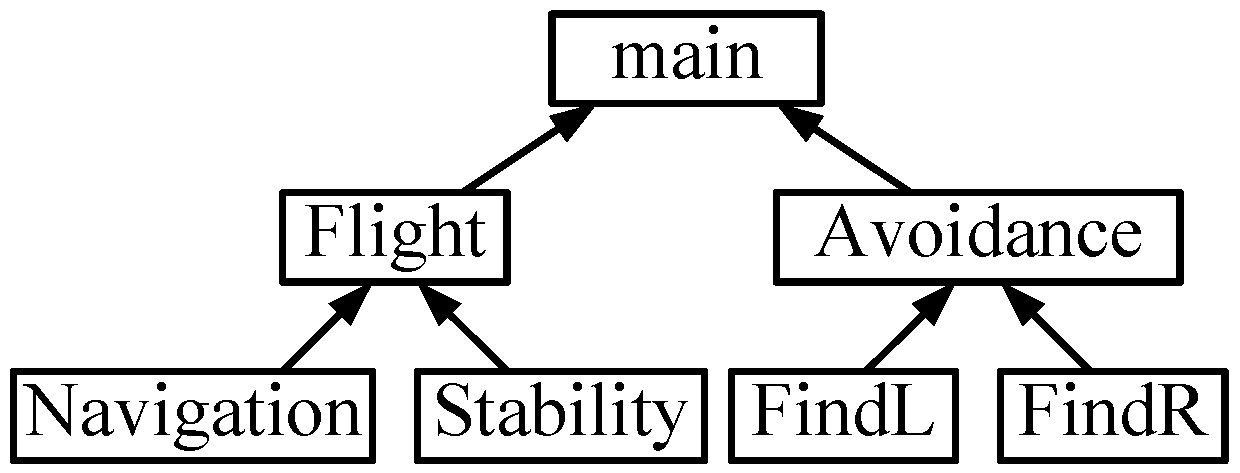
\includegraphics[width=0.4\columnwidth]{uav_genealogy_hierarchy}
		\label{fig:forec:uav_genealogy_hierarchy}
	}
	\hfill
	\subfloat[Descriptive examples.] {
		\begin{minipage}[b]{0.55\textwidth}
			\texttt{main}: Parent of \texttt{Flight} and \texttt{Avoidance}.		\\
			\texttt{Flight}: Parent of \texttt{Navigation} and \texttt{Stability}.	\\
			\texttt{main} and \texttt{Flight}: Ancestors of \texttt{Navigation} and \texttt{Stability}.	\\
			\texttt{FindL} and \texttt{FindR}: Siblings of each other.				\\
			\texttt{Navigation}: Relative of \texttt{Avoidance}, \texttt{FindL}, \texttt{FindR}, and \texttt{Stability}.
		\end{minipage}
		\label{fig:forec:uav_genealogy_description}
	}
	
	\caption{Thread genealogy for Figure~\ref{fig:forec:uav}.}
	\label{fig:forec:uav_genealogy}
\end{figure}


%-----------------------------------------------------------------------------

\subsubsection{Shared Variables}
\label{sec:forec:shared_variables}
All variables in ForeC follow the scoping rules of C. By
default, all variables are \emph{private} and can only be
accessed (read or write) by one thread throughout its scope.
To allow a variable to be accessed by multiple threads, it
must be declared as a \emph{shared} variable by using the
\verb$shared$ type qualifier. Thus, any misuse of private variables are
easy to detect at compile time. Appendix~\ref{sec:forec_combine:passing}
describes how shared variables are passed by value and by reference into
functions. The semantics we propose for 
ForeC makes sure that the shared variables can be safely accessed
by the parallel threads without the need
of mutual exclusion constructs. The goal is to provide a
deterministic shared variable semantics that is agnostic to
scheduling, which is essential for the design and
debug of parallel programs. Within each tick, the accesses
to a shared variable from two threads may occur in sequence or 
in parallel:
\begin{definition}
	\label{def:forec:access_sequential}
	Accesses from two threads are in \emph{sequence} if both 
	threads are not relatives or if the accesses occur in different ticks. 
\end{definition}

\begin{definition}
	\label{def:forec:access_parallel}
	Accesses from two threads are in \emph{parallel} if both 
	threads are relatives and the accesses occur in the same tick.
\end{definition}

Improperly managed parallel accesses to a shared variable
can cause race conditions, leading to non-deterministic 
behavior. For example, two parallel writes to a
shared variable can non-deterministically and partially
overwrite each other's value. A parallel read and write to a
shared variable can result in the read returning the
variable's value before, during, or after the write has
completed. Table~\ref{table:literature:mutual_exclusion} 
in Section~\ref{sec:literature} reviewed 
the solutions that exist for enforcing mutual
exclusion on shared variables, usually by
interleaving parallel accesses into a sequence.
Parallel accesses can be interleaved in many ways
(influenced by the programmer, compiler, and runtime system),
and relying on a particular interleaving for correct program
behavior is brittle and error prone.

%\begin{table}
%	\centering
%
%	\begin{tabular}{| c  c | c | c |}
%		\cline{3-4}
%		\multicolumn{1}{c}{}																& 				& \multicolumn{2}{p{5.8cm} |}{\textbf{Accesses to the shared variable are by relative threads?}}	\\ 
%		\multicolumn{1}{c}{}																& 				& \textbf{Yes}		& \textbf{No}																\\ \cline{1-4}
%		\multirow{2}{6.3cm}{\textbf{Accesses to the shared variable are in the same tick?}}	& \textbf{Yes}	& Parallel Access	&																			\\ \cline{2-3} 
%																							& \textbf{No}	& \multicolumn{2}{c|}{Sequential Access}														\\
%		\hline
%	\end{tabular}
%	\caption{Determining whether two accesses to a shared variable are parallel or sequential.}
%	\label{table:forec:variable_access}
%\end{table}

We propose a shared memory model that permits shared 
variables to be accessed deterministically in parallel, without 
needing the programmer to explicitly use mutual exclusion. 
%PC-MoC is similar in spirit to the sequentially constructive model of 
%computation (SC-MoC)~\cite{timed_seq_concurrency} but targets the 
%execution of synchronous threads on parallel architectures. 
The goals of the model are: 
\begin{description}
	\item[Isolation] Provide isolation between threads to enable the local reasoning of each thread.
		  That is, the execution of a thread's local tick can be understood by only knowing 
		  the values of the variables at the start of the thread's local tick.

	\item[Determinism~\cite{Maraninchi92}] Ensure deterministic execution regardless of scheduling decisions. This guarantees 
		  that deterministic outputs are always generated at the end of each tick.

	\item[Parallelism] Minimize the need to serialize parallel accesses to shared variables. This
		  maximizes the amount of parallel execution that can occur at runtime, which is important 
		  for improving the program's performance.
\end{description}
We propose the following mechanisms for achieving our shared memory model: 
All threads access their own \emph{local copies} of the shared variables, and these 
copies are \emph{resynchronized} every time threads join and when the tick ends.

\subsubsection{Copying of Shared Variables}
\label{sec:forec:shared_variables_copying}
Every time a thread starts its local tick, it creates
\emph{local copies} of all the shared variables that its body
accesses (reads or writes). 
When a thread is forked, its initial copy of a shared variable 
is created from its parent's copy if it exists, otherwise, from 
the shared variable's resynchronized value.
A parent thread that is blocked on a \verb$par$ statement
does not create any copies of the shared variables until 
the \verb$par$ statement terminates. For example, in tick 
two of Figure~\ref{fig:forec:uav_timing1}, the threads 
\texttt{main}, \texttt{Flight}, and \texttt{Avoidance} 
make no local copies. The child threads \texttt{Navigation}, 
\texttt{Stability}, \texttt{FindL}, and \texttt{FindR} must
create their local copies from the shared variables' resynchronized
values, e.g., \texttt{obst}~=~2 and \texttt{newPos}~=~56. 
%Shared variables can be passed as arguments into threads
%(Appendix~\ref{sec:forec_combine:passing}). Following the C
%convention, when a shared variable is \emph{passed by value}, 
%only its value is used to initialize the thread's parameter.
A shared variable declared inside a thread can be shared
among its child threads by \emph{passing a reference} (using a
pointer) into the child threads
(e.g., \verb$obst$ on line~\ref{code:forec:uav_par1} of
Figure~\ref{fig:forec:uav}). When a shared variable is
passed by reference into an ordinary function (e.g.,
\verb$obst$ on line~\ref{code:forec:uav_while2}), the 
function uses the calling thread's copy of the shared variable. 

\subsubsection{Resynchronization of Shared Variables}
\label{sec:forec:shared_variables_resync}
The copies are \emph{resynchronized} every time the program
completes its tick (before outputs are emitted).
Resynchronizing at specific program points ensures that the
semantics of shared variables is agnostic to scheduling. 
We use combine functions to compute the value of resynchronized
shared variables. Combine functions must be
deterministic, associative, and commutative. That
is, the combine function produces the same outputs from the
same inputs, regardless of previous invocations and how the
copies are ordered or grouped. The signature of any combine
function is 
$\mathit{C}: \mathit{Val} \times \mathit{Val} \to \mathit{Val}$. 
The two input parameters are the two
copies to be combined. 
When a \verb$par$ statement terminates, the copies
from the terminating child threads are combined and
assigned to their parent thread's copies of shared variables.
For example, in Figure~\ref{fig:forec:uav_timing1}, the \verb$Avoidance$
thread gets a copy of \verb$obst$ every time \verb$FindL$ and 
\verb$FindR$ terminate. Appendix~\ref{sec:forec_combine} 
describes more examples of combine functions and how more than 
two copies are combined. 

It can be useful to ignore some of the copies when
resynchronizing a shared variable. This is achieved by
specifying a \emph{combine policy} that determines what
copies will be ignored. The combine policies are \verb$new$,
\verb$mod$, and \verb$all$. The combine policy of a shared
variable is specified during variable declaration in the
\verb$combine$ clause, e.g., \verb$combine new with$. The
\verb$new$ policy ignores copies that have the same
value as their shared variable, i.e., which has not changed during 
the tick. 
The \verb$mod$ policy ignores copies that were
not assigned a value during the tick, i.e., have not appeared on
the lefthand side of an assignment.\footnote{This differs 
from the \texttt{new} policy because an assignment 
of the form ``\texttt{x=x}'' will be taken into account by the 
\texttt{mod} policy, but not by the \texttt{new} policy.} The default policy is
\verb$all$ where no copies are ignored. Note that the
combine function is not invoked when only one copy remains.
Instead, that copy becomes the resynchronized value. 
Appendix~\ref{sec:forec_combine} provides extensive 
illustrations comparing the behavior of the combine policies.

%Often, a shared variable is intentionally used where only
%one thread writes to it and the other threads read from it. Its
%combine function would never be invoked if the \verb$new$
%or \verb$mod$ combine policy is used. As a shorthand, the
%\verb$combine$ clause can be dropped from a shared
%variable's declaration if 1) the \verb$new$ or \verb$mod$
%combine policy is used, and 2) it can be statically 
%proved that parallel threads will not write to it. A proof 
%may not always be possible because some writes to the shared 
%variable may be executed conditionally by \verb$if$-statements 
%or loops. The compiler can make the conservative assumption 
%that all conditional writes to a shared will always occur.
%Line~\ref{code:forec:uav_newpos} in
%Figure~\ref{fig:forec:uav} is an example of this
%shorthand.


%-----------------------------------------------------------------------------

\subsubsection{Hierarchical Preemption}
\label{sec:forec:preemption}

\begin{figure}
	\centering
	\footnotesize
	\def\arraystretch{1.3}
	
	\begin{tabular}{| l l l|}
		\hline
		\textbf{Expressions:}	& ~~~\emph{exp}  ::= \emph{val} \textbar{} \emph{var} \textbar{} \emph{ptr}\verb$[$\emph{exp}\verb$]$ \textbar{} \verb$($\emph{exp}\verb$)$ 					& \emph{// Constants, variables, and grouping.}	\\
								&			~~~~~~~~~~\textbar{} \emph{u\_op} \emph{exp} \textbar{} \emph{exp} \emph{b\_op} \emph{exp}															& \emph{// Unary and binary expressions.}		\\
		\textbf{Unary}			&																																								&												\\
		\textbf{Operators:}		& \emph{u\_op}	 ::= \verb$*$ \textbar{} \verb$&$ \textbar{} \verb$!$ \textbar{} \verb$-$ \textbar{} \verb$~$										 			& \emph{// Indirection, address, negation,}		\\
								&																																								& \emph{~~~~~~~negative, and one's complement.}	\\
		\textbf{Binary}			&																																								&												\\
		\textbf{Operators:}		& \emph{b\_op}	 ::= \verb$||$ \textbar{} \verb$&&$ \textbar{} \verb$^$ \textbar{} \verb$|$ \textbar{} \verb$&$ \textbar{} \verb$<<$ \textbar{} \verb$>>$ 		& \emph{// Logical and bitwise operators.}		\\
								&			~~~~~~~~~~\textbar{} \verb$==$ \textbar{} \verb$!=$ \textbar{} \verb$<$ \textbar{} \verb$>$ \textbar{} \verb$<=$ \textbar{} \verb$>=$				& \emph{// Relational operators.}				\\
								&			~~~~~~~~~~\textbar{} \verb$+$ \textbar{} \verb$-$ \textbar{} \verb$*$ \textbar{} \verb$/$ \textbar{} \verb$%$										& \emph{// Arithmetic operators.}				\\
		\hline
	\end{tabular}
	
	\caption{Syntax of preemption conditions.}
	\label{fig:forec:abort_expressions}
\end{figure}

\begin{figure}
	\centering

	\begin{minipage}[t]{0.67\columnwidth}
		\lstinputlisting[style=full]{./code/forec/informal/uav_abort.forec}
	\end{minipage}

	\caption{Figure~\ref{fig:forec:uav} extended with preemption.}
	\label{fig:forec:uav_abort}
\end{figure}

\begin{figure}
	\centering

	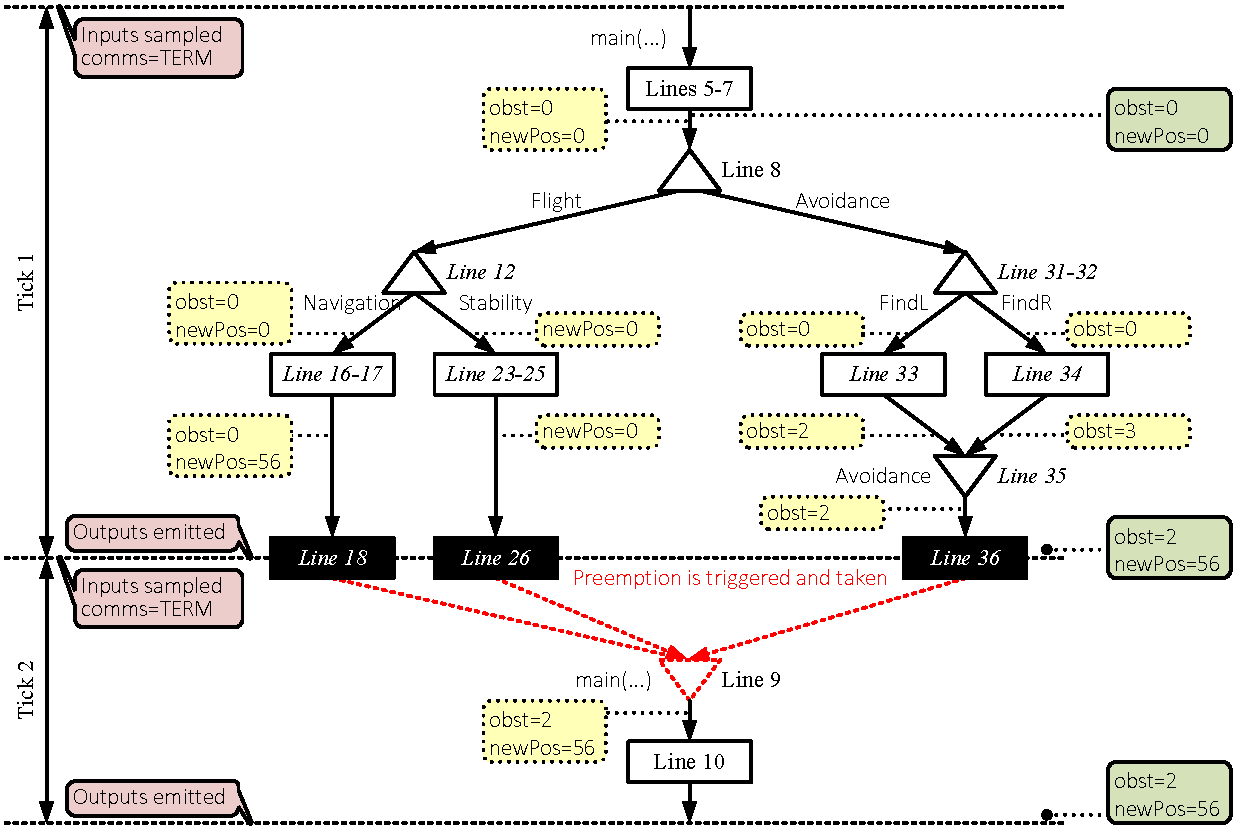
\includegraphics[width=\columnwidth]{images/uav_timing2.pdf}

	\caption{Possible execution trace for Figure~\ref{fig:forec:uav_abort}.}
	\label{fig:forec:uav_timing2}
\end{figure}

Inspired by Esterel~\cite{timed_esterel}, the
\verb$abort$~\emph{st} \verb$when$~(\expression{}) statement
provides preemption~\cite{timed_preemption}, which is the
termination of the \verb$abort$ body \emph{st} when the
condition \expression{} evaluates to \emph{true}. Preemption
can be used to model state machines succinctly. The
condition \expression{} must be a side-effect free
expression produced from the syntax shown 
in Figure~\ref{fig:forec:abort_expressions}. 
In Figure~\ref{fig:forec:uav_abort},
the \verb$main$ function of the UAV has been extended to
respond to external commands through the input 
\verb$comms$ (line~\ref{code:forec:uav_abort_comms}). 
The value of \verb$comms$ can be \verb$OK$, \verb$ERROR$, 
\verb$WARN$, or \verb$TERM$ (line~\ref{code:forec:uav_abort_state}).
The \verb$abort$ statement on
line~\ref{code:forec:uav_abort_abort} preempts the 
execution of all the UAV tasks when \verb$TERM$
is received. A possible execution trace of the 
program of Figure~\ref{fig:forec:uav_abort} is given in
Figure~\ref{fig:forec:uav_timing2}. The \emph{italicized}
line numbers in Figure~\ref{fig:forec:uav_timing2} refer 
to the line numbers in Figure~\ref{fig:forec:uav}, while 
the non-italicized line numbers refer to the line numbers in 
Figure~\ref{fig:forec:uav_abort}. We now explain the semantics of
the \verb$abort$ statement. The preemption of the
\verb$abort$ must be \emph{triggered} before the \verb$abort$
body can be terminated. Preemption is never taken when the
\verb$abort$ body executes for the first time (e.g., tick
one in Figure~\ref{fig:forec:uav_timing2}). At the start of
each subsequent tick, the condition \expression{} is
evaluated before the \verb$abort$ body can execute. This
allows shared variables in the condition to be evaluated
with their resynchronized value. If \expression{} 
evaluates to \emph{true} (any non-zero value following the C
convention), then the preemption is triggered and the
\verb$abort$ statement is terminated. At the start of tick
two in Figure~\ref{fig:forec:uav_timing2}, preemption is
triggered because the preemption condition evaluates to \emph{true}.
The \verb$abort$ statement also terminates if its body
terminates normally. 

Preemptions in ForeC differ from those in Esterel because
Esterel uses signals for thread communication rather than 
shared variables. As explained in
Section~\ref{sec:introduction:synchronous}, signals in
Esterel are either present or absent in each tick and this
information is propagated instantaneously among the threads
without delay. Thus, preemptions in Esterel are triggered
instantaneously, whereas preemptions in ForeC are triggered
with a delay of one tick because the condition 
\expression{} is evaluated using values computed 
in the previous tick. Like
Esterel~\cite{timed_preemption}, the optional \verb$weak$
and \verb$immediate$ keywords change the temporal behavior
of preemptions. The \texttt{weak} keyword delays the
termination of the \texttt{abort} body until the body
cannot execute any further, e.g., reaches a \texttt{pause}
statement. The \texttt{immediate} keyword allows preemption to be
triggered immediately when execution reaches the 
\texttt{abort} for the first time. That is, the preemption condition
\expression{} is evaluated immediately when execution
reaches the \texttt{abort}. This is similar to Esterel's
\texttt{immediate} \texttt{abort} behavior.
To illustrate these four different preemption 
behaviors, Figure~\ref{fig:forec:aborts_abort} 
presents an \texttt{abort} with the optional keywords commented out. 
\begin{description}
	\item[Non-immediate and strong \texttt{abort}] The \texttt{weak} and 
		  \texttt{immediate} keywords are commented out in 
		  Figure~\ref{fig:forec:aborts_abort}. This gives the default preemption
		  behavior, summarized in Figure~\ref{fig:forec:aborts_strong}.
		  In tick one, the
		  \texttt{main} thread sets its copy of \texttt{s} to 1 and prints
		  ``1''. Next, the threads \texttt{t0} and \texttt{t1} set their
		  copies of \texttt{s} to 2 and 5, respectively. When the tick
		  ends, using the combine policy \texttt{all}, the
		  resynchronized value of \texttt{s} is 7. In tick two, the
		  \texttt{abort}'s preemption is triggered and the \texttt{abort}
		  body is terminated, resulting in ``7'' being printed. 
	
	\item[Non-immediate and weak \texttt{abort}] Only the \texttt{weak} 
		  keyword is uncommented in Figure~\ref{fig:forec:aborts_abort}.
		  Figure~\ref{fig:forec:aborts_weak} summarizes the preemption
		  behavior. The execution of tick one proceeds identically to 
		  the non-immediate and strong \texttt{abort} variant. In tick two, 
		  the \texttt{abort}'s preemption is triggered. However, the termination
		  of the \texttt{abort} body is delayed until threads \texttt{t0} and 
		  \texttt{t1} complete their local ticks.
		  This allows \texttt{t0} and \texttt{t1} to set their copies 
		  of \texttt{s} to 3 and 6, respectively. Thus, ``9''
		  is printed.
	
	\item[Immediate and strong \texttt{abort}] Only the \texttt{immediate} 
		  keyword is uncommented in Figure~\ref{fig:forec:aborts_abort}.
		  Figure~\ref{fig:forec:aborts_immediate} summarizes the 
		  preemption behavior. In tick one, the \texttt{main} thread sets
		  its copy of \texttt{s} to 1 and prints ``1''. Next, the
		  \texttt{abort}'s preemption condition is evaluated immediately.
		  Intuitively, because ``1'' was printed for the value of 
		  \texttt{s}, the condition \texttt{s>0} should
		  evaluate to \emph{true}. The counter-intuitive result of 
		  \emph{false} would occur if the resynchronized value of \texttt{s} 
		  was used. Thus, when execution reaches an immediate
		  \texttt{abort}, the condition \expression{} is evaluated 
		  immediately with the thread's copies of the shared variables. 
		  In subsequent ticks, the resynchronized values of the shared 
		  variables are used. In tick one of Figure~\ref{fig:forec:aborts_immediate}, 
		  because the preemption has been triggered, the 
		  \texttt{abort} body is terminated without executing.
	
	\item[Immediate and weak \texttt{abort}] Both the \texttt{weak} and
		  \texttt{immediate} keywords are uncommented in 
		  Figure~\ref{fig:forec:aborts_abort}. 
		  Figure~\ref{fig:forec:aborts_immediate_weak} summarizes the
		  preemption behavior. In tick one, the \texttt{main} thread sets
		  its copy of \texttt{s} to 1 and prints ``1''. Next, the
		  \texttt{abort}'s preemption is triggered immediately. However,
		  the termination of the \texttt{abort} body is delayed until 
		  threads \texttt{t0} and \texttt{t1} complete their local ticks.
		  This allows \texttt{t0} and 
		  \texttt{t1} to set their copies of \texttt{s} to 2 and 5, respectively.
		  Hence, ``7'' is printed.
\end{description}

\begin{figure}
	\centering
	
	\subfloat[Example code.] {
		\begin{minipage}[b]{0.6\textwidth}
			\lstinputlisting[style=full]{./code/forec/informal/abort.forec}
		\end{minipage}
		\label{fig:forec:aborts_abort}
	}
	
	\subfloat[Non-immediate and strong \texttt{abort}.] {
		\footnotesize
		\def\arraystretch{1.3}
		\begin{tabular}{| p{0.4\textwidth} |}
			\hline
			{\bf Tick 1:}	``1'' printed.										
							\texttt{s} = \texttt{plus}(2,5) = 7.				\\ \hline
			{\bf Tick 2:}	Preemption is triggered and the						
							\texttt{abort} body is terminated.					
							``7'' printed.										\\
																				\\
			\hline
		\end{tabular}
		\label{fig:forec:aborts_strong}
	}
	\hfill
	\subfloat[Non-immediate and weak \texttt{abort}.] {
		\footnotesize
		\def\arraystretch{1.3}
		\begin{tabular}{| p{0.4\textwidth} |}
			\hline
			{\bf Tick 1:}	``1'' printed.										
							\texttt{s} = \texttt{plus}(2,5) = 7.				\\ \hline
			{\bf Tick 2:}	Preemption is triggered. 							\\
							\texttt{s} = \texttt{plus}(3,6) = 9.				
							The \texttt{abort} body is terminated. ``9'' printed.\\ 
			\hline
		\end{tabular}
		\label{fig:forec:aborts_weak}
	}

	\subfloat[Immediate and strong \texttt{abort}.] {
		\footnotesize
		\def\arraystretch{1.3}
		\begin{tabular}{| p{0.4\textwidth} |}
			\hline
			{\bf Tick 1:}	``1'' printed. Preemption is						
							triggered and the \texttt{abort} body is terminated.
							``1'' printed again.								\\
			\hline
		\end{tabular}
		\label{fig:forec:aborts_immediate}
	}
	\hfill
	\subfloat[Immediate and weak \texttt{abort}.] {
		\footnotesize
		\def\arraystretch{1.3}
		\begin{tabular}{| p{0.4\textwidth} |}
			\hline
			{\bf Tick 1:}	``1'' printed. Preemption is							
							triggered. \texttt{s} = \texttt{plus}(2,5) = 7.	
							The \texttt{abort} body is terminated. ``7'' printed.\\
			\hline
		\end{tabular}
		\label{fig:forec:aborts_immediate_weak}
	}

	\caption{Abort variants.}
	\label{fig:forec:aborts}
\end{figure}

%For weak aborts, we choose not to check the preemption 
%after the abort body cannot execute any further. 
%This is because, if the preemption
%condition has shared variables, all the nested threads 
%would have to finish executing first before the values of
%the shared variables can be resolved to check the preemption
%condition. This would severely reduce the program's parallelism.
%In addition, for two nested weak abort statement with the
%same preemption condition, the outer condition can evaluate
%to a different value than the inner condition. The execution
%of code between the checking of the preemption conditions
%can change the state of the variables.

%If a statement should only be executed after an \verb$abort$ 
%has preempted, then the 
%``\verb$weak$?~\verb$abort$~$st_0$~\verb$when immediate$?~(\expression{})~\verb$do$~$st_1$''
%variant should be used. The statement $st_1$ in the 
%``\verb$do$~$st_1$'' clause is only after a preemption is taken. 
%If the body terminates 
%normally, then $st_1$ is not executed. This allows
%$st_1$ to be used to implement \emph{cleanup} code.
%This \verb$abort-do$ variant can be structurally translated into an 
%ordinary \verb$abort$:
%\begin{lstlisting}[style=snippet]
%int preempted=0;
%weak? abort st(*$_1$*) when immediate? (preempted=exp);
%if (preempted) {st(*$_2$*);}
%\end{lstlisting}
%where \verb$preempted$ is a uniquely defined variable.

\begin{figure}
	\centering

	\begin{minipage}[t]{0.65\columnwidth}
		\lstinputlisting[style=full]{./code/forec/informal/aborts_nested.forec}
	\end{minipage}

	\caption{Nesting of preemptions.}
	\label{fig:forec:aborts_nested}
\end{figure}

The \verb$abort$ statements can be nested to create 
a hierarchy of preemptions with the outer abort executing 
before the inner aborts. Thus, the preemption 
behavior of the outer \verb$abort$ takes precedence 
over the inner \verb$abort$s. Figure~\ref{fig:forec:aborts_nested}
is an example of an immediate and weak
\verb$abort$ (line~\ref{code:forec:aborts_nested_outer}) 
with a nested immediate and strong \verb$abort$
(line~\ref{code:forec:aborts_nested_inner}).
In tick one, preemption is triggered for the outer
weak \verb$abort$. The variable \verb$x$ is set to 2
and the inner strong \verb$abort$ preempts
immediately without executing its body. Next, \verb$x$ is set to 5 and the 
outer weak \verb$abort$ takes its preemption when 
it reaches the \verb$pause$ on line~\ref{code:forec:aborts_nested_pause}. 
Finally, ``5'' is printed.


%-----------------------------------------------------------------------------

\subsubsection{Bounded Loops}
\label{sec:forec:programming}
In addition to the strict C-coding guidelines described in 
Section~\ref{sec:introduction:programming_safety}, 
ForeC forbids the use of \emph{unbounded recursion} of function calls and 
thread forking to ensure static WCRT analyzability. 
The synchrony hypothesis requires each tick to execute 
in finite time, which means that all statements 
need to have bounded execution times. Unfortunately, loop constructs 
(\verb$for$ and \verb$while$) can have unbounded iterations, leading to
unbounded execution times. Thus, if a loop construct is used, 
then the programmer must guarantee that it always terminates or executes
a \verb$pause$ in each iteration. 
Guaranteeing that a loop always executes a \verb$pause$ may not be 
possible when \verb$pause$ statements are enclosed by \verb$if$-statements. 
The compiler makes conservative assumptions to prove whether 
a loop always executes a \verb$pause$ in each iteration. For example, 
a loop is assumed to always execute a \verb$pause$ in each iteration if 
its body has at least one statement that always executes a \verb$pause$. 
An \verb$if$-statement is assumed to always execute a \verb$pause$ if both 
its branches always execute a \verb$pause$. An 
\verb$abort$ statement is assumed to never execute a \verb$pause$. A 
\verb$par$ statement is assumed to always execute a \verb$pause$ if at 
least one of its child threads always executes a \verb$pause$. The compiler
can perform structural induction on the program's control-flow to conservatively 
prove whether every loop in the program will always execute a \verb$pause$ 
in each iteration.

\begin{table}
	\centering
	\def\arraystretch{1.3}
	
	\tbl{Structural translations of bounded loops.\label{table:forec:loop_translations}}{
		\begin{tabular}{| l | l |}
			\hline
			\textbf{Bounded Loop}					& \textbf{Translation}													\\ 
			\hline
			\texttt{for (init; cond; update) \#n \{st\}}	& \texttt{int cnt=0;}											\\
															& \texttt{for (init; cond \&\& (cnt<n); (update,cnt++)) \{st\}}	\\ \hline
			\texttt{while (cond) \#n \{st\}}				& \texttt{for ( ; cond;) \#n \{st\}}							\\ \hline
			\texttt{do \{st\} while (cond) \#n}				& \texttt{int first=1;}											\\
															& \texttt{for ( ; cond \&\& (first==0); first=0) \#n \{st\}}	\\ \hline
		\end{tabular}
	}
\end{table}


Inspired by \pretc{}~\cite{pret_pretc}, 
we have extended the syntax of loops to also allow 
the programmer to write 
bounded loops, shown in the first column of Table~\ref{table:forec:loop_translations}. 
The ``\verb$#n$'' after the loop header specifies 
that only up to \verb$n$ iterations can be executed.
The second column of Table~\ref{table:forec:loop_translations}
gives the structural translation of bounded loops. 
%For the translation of a bounded \verb$for$-loop,
%the variable \verb$cnt$ tracks the number of iterations that have 
%executed. The condition \verb$(cnt<n)$ guarantees that 
%only up to \verb$n$ iterations are executed. The bounded 
%\verb$while$-loop is translated into a bounded \verb$for$-loop. 
%For the translation of a bounded \verb$do$--\verb$while$-loop, 
%the variable \verb$first$ is used to delay the evaluation of 
%\verb$cond$ to the second iteration. This delay emulates the 
%execution behavior of a \verb$do$--\verb$while$-loop. 


%\section{The Formal Semantics of ForeC}
\subsection{Semantics of ForeC}
\label{sec:forec_semantics}
This section presents the semantics of ForeC as rewrite rules
in the style of structural operational semantics (SOS)~\cite{semantics_sos}. 
The semantics is inspired by that of other synchronous programming
languages (Esterel~\cite{timed_compiling_esterel} and \pretc{}~\cite{pret_pretc} in particular).
The semantics is defined on a set of primitive ForeC constructs
(the kernel of Table~\ref{table:forec_kernel}) from which the full ForeC 
constructs are derived. The kernel constructs are not used for compiling
and only consider a subset of the C language: the assignment operator (\verb$=$), 
the statement terminator (\texttt{;}) for sequencing,
and the \verb$if$ and \verb$while$ statements. 
Table~\ref{table:forec_structural_translations} shows how the
ForeC constructs (Table~\ref{table:forec:semantics}) are translated into the kernel 
constructs (Table~\ref{table:forec_kernel}). This is exemplified by the 
translation of the ForeC constructs in Figure~\ref{fig:transform_forec_refactored} 
into the kernel constructs in Figure~\ref{fig:transform_forec_kernel}. 
The translations for \verb$input$, \verb$output$, and \verb$pause$ are
straightforward. A \verb$shared$ variable is translated into
a global variable and a \verb$copy$ kernel statement that is placed at
the start of every thread body in the scope of the shared variable.
The \verb$copy$ kernel statement initiates the copying of the shared 
variables when the threads are forked and when the threads
start their local ticks.
The \verb$par$ statement is translated by prefixing each
thread body \body{} with a unique identifier \thread{} to 
allow the semantics to distinguish the body of one thread from another. 
The \verb$par$ kernel statement handles the resynchronization of the shared variables.
Traditionally, \verb$trap$s~\cite{timed_compiling_esterel} are used 
to translate \verb$abort$s and other complex preemption statements. 
In contrast, a simpler \verb$abort$ translation is 
possible in ForeC because \verb$abort$ is the only type of preemption statement.
Each \verb$abort$ is assigned a unique identifier $a$ and 
translated into the \verb$status$ and \verb$abort$ kernel
statements. The \verb$status$ kernel statement is needed to
define the immediate behavior of an \verb$abort$ and it takes the
unique identifier $a$ and an expression. The expression is
0 (zero) for a non-immediate \verb$abort$, but is \expression{}
(the preemption condition) for an immediate \verb$abort$. The
\verb$abort$ kernel statement takes the unique
identifier $a$ and the \verb$abort$ body~\body{}. The following section
describes the assumptions on ForeC kernel programs to 
simplify the presentation of the formal semantics. The notations, 
semantic functions, and rewrite rules are then presented.

\begin{table}
	\centering
	\def\arraystretch{1.3}
	
	\tbl{ForeC kernel constructs.\label{table:forec_kernel}}{
		\begin{tabular}{p{3cm} l}
			\bf{Kernel Construct}										& \bf{Short Description}			\\ 
			\hline
			\texttt{nop}												& Empty statement					\\
			\body{}\texttt{;}~\body{}									& Sequence operator					\\
			\var{}~\texttt{=}~\expression{}								& Assignment operator				\\
			\texttt{while}~(\expression{})~\body{}						& Loop								\\
			\texttt{if}~(\expression{})~\body{}~\texttt{else}~\body{}	& Conditional						\\
			\texttt{copy}												& Creates copies of shared variables\\
			\texttt{pause}												& Barrier synchronization			\\
			\texttt{par}(\thread{}:\body{},~\thread{}:\body{})			& Fork/join parallelism				\\
			\texttt{status}($a$, \expression{})							& Initial preemption status			\\
			\texttt{weak}?~\texttt{abort}($a$, \body{})					& Abort								\\
		\end{tabular}
	}
	
	\begin{tabnote}
		\Note{Note:}{
			\body{} is an arbitrary composition of kernel 
			constructs, \var{} is a variable, \expression{} is an expression, $t$ is a thread 
			identifier, and $a$ is an abort identifier. A question mark means that the 
			preceding symbol is optional.
		}
	\end{tabnote}
\end{table}
	
\begin{table}
	\centering
	\def\arraystretch{1.3}
	
	\tbl{Structural translations of the ForeC constructs (Table~\ref{table:forec:semantics}) to kernel constructs (Table~\ref{table:forec_kernel}).\label{table:forec_structural_translations}}{
		\begin{tabular}{| l | p{8cm} |}
			\hline
			\bf{ForeC Construct}															& \bf{ForeC Kernel Constructs}																\\ 
			\hline
			\texttt{input} and \texttt{output}												& Translated into global variables.															\\ \hline
			\texttt{shared}																	& Translated into global variables and \texttt{copy} kernel statements that are placed at 
																							  the start of every thread body.															\\ \hline
			\texttt{pause}																	& \texttt{pause}																			\\ \hline
			\texttt{par}(\body{}, \body{})													& \texttt{par}(\thread{}:\body{}, \thread{}:\body{})										\\ \hline
			\texttt{weak}?~\texttt{abort}~\body{}~\texttt{when}~(\expression{})				& \texttt{status}($a$, 0)\texttt{;} \texttt{weak}?~\texttt{abort}($a$, \body{})				\\ \hline
			\texttt{weak}?~\texttt{abort}~\body{}~\texttt{when immediate}~(\expression{})	& \texttt{status}($a$, \expression{})\texttt{;} \texttt{weak}?~\texttt{abort}($a$, \body{})	\\ \hline
		\end{tabular}
	}
\end{table}

\begin{figure}
	\centering 
	\subfloat[Original program.] {
		\begin{minipage}[b]{0.48\textwidth}
			\lstinputlisting[style=full]{./code/forec/formal/transform_forec_original.forec}
			\label{fig:transform_forec_original}
		\end{minipage}
	}
	\hfill
	\subfloat[Transformed program.] {
		\begin{minipage}[b]{0.43\textwidth}
			\lstinputlisting[style=full]{./code/forec/formal/transform_forec_refactored.forec}
			\label{fig:transform_forec_refactored}
		\end{minipage}
	}

	\subfloat[Translated kernel program.] {
		\begin{minipage}[b]{0.59\textwidth}
			\lstinputlisting[style=full]{./code/forec/formal/transform_forec_kernel.forec}
			\label{fig:transform_forec_kernel}
		\end{minipage}
	}
	
	\caption{Example of transforming and translating a ForeC program into the kernel constructs.}
	\label{fig:transform_forec}
\end{figure}


\subsubsection{Assumptions}
\label{sec:forec_semantics:assumptions}
We make the following assumptions about ForeC programs. 
(1) All programs follow safety-critical coding practices,
as discussed in Sections~\ref{sec:introduction:programming}
and \ref{sec:forec:overview}.
Dynamic memory allocation (e.g., \texttt{malloc}) and unstructured 
jumps (e.g., \texttt{goto}) cannot be used, and loops must be bounded. 
Moreover, C expressions may only be constants, variables, 
pointers, and arrays composed with the logical, bitwise, relational, 
and arithmetic operators of C. Arguments of functions and the 
right-hand side of assignment statements must not contain any assignment
operators. The sequencing operator ``\texttt{,}'' of C must not be used. These 
assumptions limit us to a deterministic subset of the C language. 
(2) All recursive function calls or forking of threads are bounded.
This assumption prevents the unbounded 
execution of functions and threads, leading to unbounded
memory use and execution time. 

To simplify the presentation of the semantics, we assume that the 
following transformations have been performed on ForeC programs. 
(1) Inlining of functions at their call sites, so that the semantics can
ignore function calls.
(2) Renaming variables uniquely and hoisting their declarations 
up to the program's global scope, so that the semantics can ignore 
(static) memory allocation and focus on the semantics of private variables 
(accessible to only one thread) and shared variables.
(3) Replacing pointers with the variables they reference, so that the 
semantics can ignore pointer analysis~\cite{BussBSE10,HardekopfL11}.
Consider the program of 
Figure~\ref{fig:transform_forec_original} that is 
transformed into the equivalent program of 
Figure~\ref{fig:transform_forec_refactored}.
The shared variable declaration for \verb$s$ 
(line~\ref{code:transform_forec_original_s} in Figure~\ref{fig:transform_forec_original}) 
is hoisted to the global scope 
(line~\ref{code:transform_forec_refactored_s} in Figure~\ref{fig:transform_forec_refactored}). 
The function \verb$f$ 
(line~\ref{code:transform_forec_original_f} in Figure~\ref{fig:transform_forec_original})
is inlined into the \verb$abort$ body 
(line~\ref{code:transform_forec_refactored_abort} in Figure~\ref{fig:transform_forec_refactored}) 
and the pointer inside \verb$f$ is replaced by the variable \verb$x$ it references.


%-----------------------------------------------------------------------------

\subsubsection{Notation}
\label{sec:forec_semantics:notation}
The rewrite rules have the following form in the style of 
structural operational semantics (SOS)~\cite{semantics_sos}:
\begin{equation*}
	\langle \StateP \rangle ~ \thread{}:\body{} 
		\xrightarrow[~~\Input~~]{k} 
	\langle \StateP' \rangle ~ \thread{}:\body{}'
\end{equation*}
This notation describes a program fragment \body{} belonging to thread \thread{},
in the program state $\StateP$ and with inputs \Input{}, which
reacts and modifies the program state to $\StateP'$, generates the 
completion code $k$, and becomes the new program fragment $\body{}'$. 
All the (globally declared) \verb$input$s are stored in \Input{}. 
Let \Thread{} be the set of all threads in the program. 
Let $\langle \StateP \rangle = \langle \Environment, \Abort \rangle$, where:
\begin{itemize}
	\item \Environment{} is an environment that maps the program's global scope to the program's global
		  variables and maps the threads' scopes to their local copies of shared variables. 
		  Specifically, \Environment{} is a partial function that maps the global 
		  scope (denoted by \Global{}) and threads ($\thread{} \in \Thread$) to a 
		  store (\Store{}) of variables. Let $\Id = \Thread \cup \{ \Global \}$, then 
		  $\Environment: \Id \hookrightarrow \Store$.
		  $\Environment[\Global]$ stores all the output, shared, and private variables
		  in the program, which are all globally declared thanks to the program 
		  transformations of Section~\ref{sec:forec_semantics:assumptions}. 
		  $\Environment[\thread{}]$ stores thread~\thread{}'s copies of shared variables. 
		  The store (\Store{}) is a partial function that maps variables ($\var \in \Var$) 
		  to values ($\val \in \Val$) and statuses ($\sts \in \Sts$), $\Store: \Var \hookrightarrow (\Val, \Sts)$. 
		  Statuses are used to define the behavior of the combine policies and
		  can be \verb$pre$ (previous resynchronized value), \verb$mod$ (modified value), 
		  \verb$cmb$ (combined value), or \verb$pvt$ (for a private variable). 
		  In $\Environment[\Global]$, the status of a private variable is always \verb$pvt$ 
		  and the status of a shared variable is always \verb$pre$. In $\Environment[\thread{}]$, 
		  a thread's copy of a shared variable always starts each local tick with
		  the status \verb$pre$.
		  		
		  For example, $\Environment = \left \lbrace \Global \to \lbrace s \to (1, \mathtt{pre}) \rbrace, t1 \to \lbrace s \to (3, \mathtt{mod}) \rbrace \right \rbrace$
		  for a program that has a shared variable \verb$s$ with value 1 in the global scope and modified
		  value $3$ in the scope of thread $t1$. We use the
		  notation $\Environment[t1][s]$ to look up the value and status $(3, \mathtt{mod})$ of \verb$s$ in $t1$'s store.
		  We use the notations $\Environment[t1][s].\val$ and $\Environment[t1][s].\sts$
		  to look up its value and status, respectively.
		  We use the notation $\StateP.\Environment$ to retrieve \Environment{} from the program state \StateP{}.
		  
	\item \Abort{} is a partial function that maps \verb$abort$ identifiers ($a \in \mathcal{A}$) 
		  to values ($\val \in \Val$) representing their preemption status, 
		  $\Abort: \mathcal{A} \to Val$. An \verb$abort$ with a non-zero value means that its
		  preemption condition is \emph{true} and that it has been triggered. 
		  
		  For example, $\Abort = \lbrace a1 \to 1, a2 \to 0 \rbrace$ 
		  for a program that has \verb$abort$s $a1$ and $a2$ with the statuses 1 and 0, respectively.
		  We use the notation $\Abort[a1]$ to look up the status of \verb$abort$~$a1$.
		  We use the notation $\StateP.\Abort$ to retrieve \Abort{} from the program state \StateP{}.
\end{itemize}
The transition of a program fragment from \body{} to $\body{}'$ 
is encoded by the completion code $k$, where:
\begin{equation*}
	k = \begin{cases}
		0		& \text{If the transition terminates.}			\\
		1		& \text{If the transition pauses.}				\\
		\bot	& \text{Otherwise (the transition continues).}
	\end{cases}
\end{equation*}


%-----------------------------------------------------------------------------
\subsubsection{Semantic Functions}
The following sections describe the semantic functions that are 
used by the rewrite rules to ensure semantic conciseness.

\subsubsection{Statically Known Information}
The following semantic functions return statically known 
information about the program:
\begin{itemize}
	\item $\GetParent(\thread{})$:
		Returns the parent of thread \thread{}.
		If $\thread{} =$ \verb$main$, then ``\verb$main$'' is returned.
	\item $\GetShared(\Global)$:
		Returns the set of all shared variables declared in the program.
	\item $\GetShared(\thread{})$:
		Returns the set of all shared variables that the body of thread \thread{} accesses (reads or writes).
	\item $\GetCombine(\var)$:
		Returns the combine function of shared variable \var{}.
	\item $\GetPolicy(\var)$:
		Returns the combine policy of shared variable \var{}.
	\item $\GetExp(a)$:
		Returns the preemption condition \expression{} of \verb$abort$ $a$.
\end{itemize}
Figure~\ref{fig:forec_predicates} exemplifies the use of these functions on
the program in Figure~\ref{fig:transform_forec_kernel}.

\begin{figure}
	\centering
	\def\arraystretch{1.3}
	
	\begin{tabular}{|l l l|}
		\hline
		$\GetParent($\verb$main$$) =$ \verb$main$	& $\GetParent($\verb$t1$$) =$ \verb$main$		& $\GetParent($\verb$t2$$) =$ \verb$main$	\\
		$\GetShared(\Global) = \{$\verb$s$$\}$		& $\GetShared($\verb$t1$$) = \{$\verb$s$$\}$	& $\GetShared($\verb$t2$$) = \{$\verb$s$$\}$\\
		$\GetCombine($\verb$s$$) =$ \verb$plus$		& $\GetPolicy($\verb$s$$) =$ \verb$all$			& $\GetExp($\verb$a1$$) =$ \verb$s>3$		\\
		\hline
	\end{tabular}
	
	\caption{Retrieving statically known information about Figure~\ref{fig:transform_forec_kernel}.}
	\label{fig:forec_predicates}
\end{figure}

\subsubsection{\sc{Eval}}
\label{sec:forec_Eval}
The semantic function $\Eval(\Environment, \Input, \id, \expression)$ 
follows the evaluation rules of C to evaluate the expression
\expression{} and return its value. 
The expression \expression{} has a classical tree structure: it can
be an atom (a constant, a variable, a string, ...), a unary
arithmetic or Boolean operation (\texttt{*}, \texttt{\&}, \texttt{!}, 
\texttt{-},~\texttt{\~}), a binary arithmetic or Boolean 
operation (\texttt{||}, \texttt{\&\&}, \texttt{\^}, 
\texttt{|}, \texttt{\&}, \texttt{<}\texttt{<}, \texttt{>}\texttt{>}, \texttt{==}, 
\texttt{!=}, \texttt{<}, \texttt{>}, \texttt{<=}, \texttt{>=}, \texttt{+},
\texttt{-}, \texttt{*}, \texttt{/},~\texttt{\%}), a function call with its arguments
passed by value and by reference, an array, and so on. For
the sake of simplicity, we do not give the details 
here~\cite{programming_languages_clight,programming_languages_cholera} and
will just write the string of the expression when calling
the $\Eval$ function. Finally, the $\Eval$ function returns the
value of \expression{}. Unlike in C, where expressions can have 
side-effects (which would be captured by the function $\Eval$
returning a \emph{pair} $(\Environment', \val)$ instead of just $\val$),
we have assumed that ForeC expressions and functions are
side-effect free. During the evaluation, a
variable's value is retrieved with the semantic function
$\GetVal(\Environment, \Input, \id, \var)$ described by
Algorithm~\ref{algo:GetVal}. The inputs to the algorithm
are: the program's environment \Environment{}, the inputs
\Input{}, the identifier \id{} of the
store to try and retrieve the value from, and the variable
\var{} of interest. The output is a value \val{}. If \var{}
is an input, then line~\ref{algo:GetVal_input} returns its 
value. Otherwise, if \var{} is in
\id{}'s store, then line~\ref{algo:GetVal_local} returns its 
value. Otherwise, line~\ref{algo:GetVal_global} returns the 
global value of \var{}.

\begin{algorithm}
	\KwIn{Program's environment \Environment{}, inputs \Input{}, identifier \id{} of the store to search, and variable \var{} of interest.}
	\KwOut{Value of \var{}.}
	
	\BlankLine
	
	\uIf(\tcp*[f]{If \var{} is an input.}){$\var \in \Input$} {
		\KwRet{$\Input[\var]$}						\tcp*{Return the input value of \var{}.}\label{algo:GetVal_input}
	} \uElseIf(\tcp*[f]{Otherwise, if a local copy of \var{} exists.}){$\var \in \Environment[\id]$} {
		\KwRet{$\Environment[\id][\var].\val$}		\tcp*{Return the value of \var{} from \id{}'s store.}\label{algo:GetVal_local}
	} \Else {
		\KwRet{$\Environment[\Global][\var].\val$}	\tcp*{Otherwise, return the global value of \var{}.}\label{algo:GetVal_global}
	}
	
	\caption{$\GetVal(\Environment, \Input, \id, \var)$: Gets the value of a given variable.}
	\label{algo:GetVal}
\end{algorithm}

\subsubsection{\sc{Copy}}
\label{sec:forec_Copy}
The semantic function $\Copy(\Environment, \thread{})$
creates in thread \thread{} the local copies of each
shared variable $\var \in \GetShared(\thread{})$ 
that it does not have. That is, if thread
\thread{} already has a copy of the shared variable
\var{}, then $\Copy$ skips the copying of \var{}.
This conditional behavior is needed because the semantic
function $\Copy$ may be invoked for a thread \thread{} that
already has a subset of its required local copies. For
example, when local copies are created for a parent thread
that is resuming from the termination of a \texttt{par}, 
the combined values from its child threads
must not be overwritten. 
The $\Copy$ function is described
by Algorithm~\ref{algo:Copy}. The inputs to the algorithm
are: the program's environment \Environment{} and a thread
\thread{}. The output is an updated environment
\Environment{}. Line~\ref{algo:Copy_retrieve} considers 
each shared variables that is accessed in the thread's 
body. For each shared
variable\footnotemark[1], line~\ref{algo:Copy_if} checks if
a copy already exists. If it does not exist, then 
lines~\ref{algo:Copy_parent_val}--\ref{algo:Copy_parent}
copy the parent thread's copy if available, 
otherwise from the shared variable 
(line~\ref{algo:Copy_global}). Line~\ref{algo:Copy_return}
returns the updated environment \Environment{}.

\footnotetext[1]{Recall from
Section~\ref{sec:forec_semantics:notation} that
\Environment{} maps the global and thread scopes to their
own store of variables, $\Environment: \Id \hookrightarrow
\Store$. Variables are mapped to a value and status,
$\Store: \Var \hookrightarrow (\Val, \Sts)$ where 
$\Sts = \{ \texttt{pre}, \texttt{mod}, \texttt{cmb}, \texttt{pvt} \}$.
A private variable has the status \texttt{pvt}, a shared
variable has the status \texttt{pre}, and a thread's copy of
a shared variable starts each local tick with the status
\texttt{pre}. The notation $\Environment[\thread{}][\var]$
looks up the value and status $(\val, \sts)$ of thread
\thread{}'s copy of \var{}.}

\begin{algorithm}
		\KwIn{Program's environment \Environment{}, and thread \thread{}.}
		\KwIn{Updated environment \Environment{}.}
		
		\BlankLine
		
		\ForAll(\tcp*[f]{For all shared variables needed by thread \thread{}.}){$\var \in \GetShared(\thread{})$} {	\label{algo:Copy_retrieve}
			\If(\tcp*[f]{If thread \thread{} does not have a copy.}){$\var \notin \Environment[\thread{}]$} {		\label{algo:Copy_if}
				\uIf(\tcp*[f]{If its parent has a copy.}){$\var \in \Environment[\GetParent(\thread{})]$} {
					$\val := \Environment[\GetParent(\thread{})][\var].\val$										\tcp*{Value of its parent's copy.}\label{algo:Copy_parent_val}
					$\Environment[\thread{}][\var \gets (\val, \texttt{pre})]$										\tcp*{Copy its parent's copy.}\label{algo:Copy_parent}
				} \Else(\tcp*[f]{Otherwise, its parent does not have a copy.}) {
					$\Environment[\thread{}][\var \gets \Environment[\Global][\var]]$								\tcp*{Copy the shared variable from the global scope.}\label{algo:Copy_global}
				}
			}
		}
		\KwRet{$\Environment$}																						\label{algo:Copy_return}
	
	\caption{$\Copy(\Environment, \thread{})$: Copies all the shared variables needed by a thread.}
	\label{algo:Copy}
\end{algorithm}

\subsubsection{\sc{Combine}}
\label{sec:forec_Combine}
The semantic function $\Combine(\Environment, \thread{1}, \thread{2}, \thread{0})$ 
combines all the copies of shared variables from two threads
and is described by Algorithm~\ref{algo:Combine}.
The inputs to the algorithm are: the program's environment
\Environment{}, two threads \thread{1} and \thread{2} to
combine, and thread \thread{0} to store the combined values.
The output is an updated environment \Environment{}. 
Line~\ref{algo:Combine_for} considers each shared variable\footnotemark[1]
\var{}.
Line~\ref{algo:Combine_pre} gets the shared variable's
\verb$pre$ value (\verb$preVal$). For the combine policy \verb$all$, the
copies from both threads are combined if they exist. Thus,
line~\ref{algo:Combine_default} gets the set of threads
\Thread{} that have a copy of the shared variable. If the
combine policy is \verb$new$, then line~\ref{algo:Combine_new} 
keeps only the copies with values that differ from the shared 
variable's \verb$pre$ value
($\Environment[\thread{}][\var].\val \neq \texttt{preVal}$) 
or copies that have been combined
($\Environment[\thread{}][\var].\sts = \texttt{cmb}$). 
If the combine policy is \verb$mod$, then line~\ref{algo:Combine_mod} 
keeps only the modified or combined copies 
($\Environment[\thread{}][\var].\sts \in \{ \texttt{mod}, \texttt{cmb} \}$). 
If two copies are
found, then line~\ref{algo:Combine_c} gets the shared 
variable's combine function (\emph{cf}) and line~\ref{algo:Combine_combine}
computes the combined value. Line~\ref{algo:Combine_assign2} 
assigns the combined value to thread \thread{0} with the
status \verb$cmb$ because it is now a combined value. 
If only one copy is found, then line~\ref{algo:Combine_assign1} 
assigns the value of that copy to thread \thread{0} with the
status \verb$cmb$. Line~\ref{algo:Combine_return} returns the 
updated environment \Environment{} restricted to \thread{0}
(i.e., without thread \thread{1} 
and \thread{2}'s store).

\begin{algorithm}
		\KwIn{Program's environment \Environment{}, threads \thread{1} and \thread{2} to combine, and thread \thread{0} to store the combined values.}
		\KwOut{Updated environment \Environment{}.}
		
		\BlankLine
		
		\ForAll(\tcp*[f]{For all shared variables.}){$\var \in \GetShared(\Global)$} {										\label{algo:Combine_for}
			$\texttt{preVal} := \Environment[\Global][\var].\val$															\tcp*{Get the \texttt{pre} of \var{}.}\label{algo:Combine_pre}
			$\Thread := \lbrace \thread{} \mid \thread{} \in \lbrace \thread{1}, \thread{2} \rbrace, \var \in \Environment[\thread{}] \rbrace$		\tcp*{Set of threads with a copy of \var{}.}\label{algo:Combine_default}
			\uIf{$\GetPolicy(\var) = \texttt{new}$} {
				\tcp{Keep only the copies that differ from \texttt{preVal} or have been combined.}
				$\Thread := \lbrace \thread{} \mid \thread{} \in \Thread, \Environment[\thread{}][\var].\val \neq \texttt{preVal} \lor \Environment[\thread{}][\var].\sts = \texttt{cmb} \rbrace$\;	\label{algo:Combine_new}
			} \ElseIf{$\GetPolicy(\var) = \texttt{mod}$} {
				\tcp{Keep only the modified or combined copies.}
				$\Thread := \lbrace \thread{} \mid \thread{} \in \Thread, \Environment[\thread{}][\var].\sts \in \{ \texttt{mod}, \texttt{cmb} \} \rbrace$\;	\label{algo:Combine_mod}
			}
			
			\BlankLine
			
			\uIf(\tcp*[f]{If there are two copies to combine.}){$\lvert \Thread \rvert = 2$} {			\label{algo:Combine_if}
				$\mathit{cf} := \GetCombine(\var)$														\tcp*{Get the combine function of \var{}.}\label{algo:Combine_c}
				$\val := cf(\Environment[\thread{1}][\var].\val, \Environment[\thread{2}][\var].\val)$	\tcp*{Combine the copies.}\label{algo:Combine_combine}
				$\Environment[\thread{0}][\var \gets (\val, \texttt{cmb}) ]$							\tcp*{Assign the combined value to \thread{0}.}\label{algo:Combine_assign2}
			} \ElseIf(\tcp*[f]{Otherwise, there is only one copy.}) {$\lvert \Thread \rvert = 1$} {
				$\Environment[\thread{0}][\var \gets (\Environment[\thread{} \in \Thread][\var].\val, \texttt{cmb}) ]$	\tcp*{Assign the only copy to \thread{0}.}\label{algo:Combine_assign1}
			}
		}
		$\Environment' = \{ (id, store) \mid (id, store) \in \Environment \land id \neq \thread{1} \land id \neq \thread{2} \}$\;
		\KwRet $\Environment'$																			\label{algo:Combine_return}
	
	\caption{$\Combine(\Environment, \thread{1}, \thread{2}, \thread{0})$: Combines the copies of shared variables from two threads.}
	\label{algo:Combine}
\end{algorithm}

\clearpage

%-----------------------------------------------------------------------------

\subsubsection{The Structural Operational Semantics}
\label{sec:forec_semantics:sos}
This section presents the operational semantics of the kernel
constructs presented in Table~\ref{table:forec_kernel}.

\subsubsection{The \texttt{nop} Statement}
The \verb$nop$ statement does nothing and terminates instantly:
\begin{equation*}
	\tag{nop}
	\label{forec:nop}
	\langle \Environment, \Abort \rangle ~ \thread{}:\mathtt{nop}
		\xrightarrow[~~\Input~~]{0} 
	\langle \Environment, \Abort \rangle ~ \thread{}:
\end{equation*}

\subsubsection{The \texttt{copy} Statement}
The \verb$copy$ statement copies the shared variables needed
by thread \thread{} and terminates instantly. The combining of 
the copies is handled by the \verb$par$ statement:
\begin{equation*}
	\tag{copy}
	\label{forec:copy}
	\langle \Environment, \Abort \rangle ~ \thread{}:\mathtt{copy}
		\xrightarrow[~~\Input~~]{0} 
	\langle \Copy(\Environment, \thread{}), \Abort \rangle ~ \thread{}:
\end{equation*}

\subsubsection{The \texttt{pause} Statement}
The \verb$pause$ statement rewrites into the \verb$copy$ statement
and pauses. The \verb$copy$ statement ensures that thread \thread{} 
starts its next local tick by copying the shared variables it needs
(the \verb$pre$ values are copied):
\begin{equation*}
	\tag{pause}
	\label{forec:pause}
	\langle \Environment, \Abort \rangle ~ \thread{}:\mathtt{pause}
		\xrightarrow[~~\Input~~]{1} 
	\langle \Environment, \Abort \rangle ~ \thread{}:\mathtt{copy}
\end{equation*}

\subsubsection{The \texttt{status} Statement}
Recall that the \texttt{abort} statement is mapped to a \texttt{status}
statement that evaluates the preemption status, followed by an invocation
of the \texttt{abort} kernel statement that accesses the result of the
evaluated preemption status.

The \verb$status$ statement sets \verb$abort$ $a$'s preemption status
to the value of the expression \expression{}, and then it terminates
instantly:
\begin{equation*}
	\tag{status}
	\label{forec:status}
	\langle \Environment, \Abort \rangle ~ \thread{}:\mathtt{status}(a, \expression)
		\xrightarrow[~~\Input~~]{0} 
	\langle \Environment, \Abort[a \gets \Eval(\Environment, \Input, \thread{}, \expression)] \rangle ~ \thread{}:
\end{equation*}

\subsubsection{The \texttt{abort} Statement}
The \verb$abort$ of $a$ executes its body \body{} if its preemption 
has not been triggered. The body may have paused ($k = 1$) or may have executed
some instantaneous statements ($k = \bot$):
\begin{equation*}
	\tag{abort-1}
	\label{forec:abort-1}
	\frac{
			\langle \Environment, \Abort \rangle ~ \thread{}:\body{}
				\xrightarrow[~~\Input~~]{k \in \lbrace 1, \bot \rbrace} 
			\langle \Environment', \Abort' \rangle ~ \thread{}:\body{}'			
		}{
			\langle \Environment, \Abort \rangle ~ \thread{}:\mathtt{weak}?~\mathtt{abort}(a, \body{})
				\xrightarrow[~~\Input~~]{k} 
			\langle \Environment', \Abort' \rangle ~ \thread{}:\mathtt{weak}?~\mathtt{abort}(a, \body{}')
		}
	(\Abort[a] = 0)
\end{equation*}
The \verb$abort$ terminates normally if its body terminates and its preemption has not
been triggered:
\begin{equation*}
	\tag{abort-2}
	\label{forec:abort-2}
	\frac{
			\langle \Environment, \Abort \rangle ~ \thread{}:\body{}
				\xrightarrow[~~\Input~~]{0} 
			\langle \Environment', \Abort' \rangle ~ \thread{}:
		}{
			\langle \Environment, \Abort \rangle ~ \thread{}:\mathtt{weak}?~\mathtt{abort}(a, \body{})
				\xrightarrow[~~\Input~~]{0} 
			\langle \Environment', \Abort' \rangle ~ \thread{}:
		}
	(\Abort[a] = 0)
\end{equation*}
The \verb$weak abort$ terminates normally if its 
body terminates, even if its preemption has been triggered:
\begin{equation*}
	\tag{abort-3}
	\label{forec:abort-3}
	\frac{
			\langle \Environment, \Abort \rangle ~ \thread{}:\body{}
				\xrightarrow[~~\Input~~]{0} 
			\langle \Environment', \Abort' \rangle ~ \thread{}:
		}{
			\langle \Environment, \Abort \rangle ~ \thread{}:\mathtt{weak}~\mathtt{abort}(a, \body{})
				\xrightarrow[~~\Input~~]{0} 
			\langle \Environment', \Abort' \rangle ~ \thread{}:
		}
	(\Abort[a] \neq 0)
\end{equation*}
The \verb$weak abort$ allows its body to execute instantaneous statements ($k = \bot$), 
even if its preemption has been triggered:
\begin{equation*}
	\tag{abort-4}
	\label{forec:abort-4}
	\frac{
			\langle \Environment, \Abort \rangle ~ \thread{}:\body{}
				\xrightarrow[~~\Input~~]{\bot} 
			\langle \Environment', \Abort' \rangle ~ \thread{}:\body{}'
		}{
			\langle \Environment, \Abort \rangle ~ \thread{}:\mathtt{weak}~\mathtt{abort}(a, \body{})
				\xrightarrow[~~\Input~~]{\bot} 
			\langle \Environment', \Abort' \rangle ~ \thread{}:\mathtt{weak}~\mathtt{abort}(a, \body{}')
		}
	(\Abort[a] \neq 0)
\end{equation*}
The \verb$weak abort$ terminates if its body pauses and its preemption has been triggered,
and then it rewrites into the \verb$copy$ statement because it may be the start of thread \thread{}'s 
local tick\footnotemark[2]:
\footnotetext[2]{\label{sec:forec_semantics:footnote2}The \texttt{abort} may have had a 
\texttt{par} statement that paused. In this case, when the \texttt{abort} kernel statement
preempts, thread \thread{} will start its local tick.}
\begin{equation*}
	\tag{abort-5}
	\label{forec:abort-5}
	\frac{
			\langle \Environment, \Abort \rangle ~ \thread{}:\body{}
				\xrightarrow[~~\Input~~]{1} 
			\langle \Environment', \Abort' \rangle ~ \thread{}:\body{}'
		}{
			\langle \Environment, \Abort \rangle ~ \thread{}:\mathtt{weak}~\mathtt{abort}(a, \body{})
				\xrightarrow[~~\Input~~]{\bot} 
			\langle \Environment', \Abort' \rangle ~ \thread{}:\mathtt{copy}
		}
	(\Abort[a] \neq 0)
\end{equation*}
The strong \verb$abort$ terminates without executing its body if its preemption has been triggered,
and then it rewrites into the \verb$copy$ statement because it may be the start of thread \thread{}'s 
local tick\footnotemark[3]:
\begin{equation*}
	\tag{abort-6}
	\label{forec:abort-6}
	\frac{
			\Abort[a] \neq 0
		}{
			\langle \Environment, \Abort \rangle ~ \thread{}:\mathtt{abort}(a, \body{})
				\xrightarrow[~~\Input~~]{\bot} 
			\langle \Environment, \Abort \rangle ~ \thread{}:\mathtt{copy}
		}
\end{equation*}

\footnotetext[3]{In addition to footnote~\ref{sec:forec_semantics:footnote2}, 
the strong preemption prevents the execution of a \texttt{copy} statement inside the abort body.}

\subsubsection{The Assignment Operator (\texttt{=})}
The assignment operator evaluates the expression
\expression{} into a value 
$\val = \Eval(\Environment, \Input, \thread{}, \expression)$.
If \var{} is a shared variable\footnotemark[4] (rule \ref{forec:assign-shared}), then the value \val{} and status \verb$mod$ 
is assigned to the thread's copy in $\Environment[\thread{}]$. 
Otherwise, if \var{} is a private variable (rule \ref{forec:assign-private}), then the value \val{}
and status \verb$pvt$ is assigned to the global variable in $\Environment[\Global]$:
\begin{equation*}
	\tag{assign-shared}
	\label{forec:assign-shared}
	\frac{
			\var \in \GetShared(\thread{})
		}{
			\langle \Environment, \Abort \rangle ~ \thread{}:\var \mathtt{=} \expression
				\xrightarrow[~~\Input~~]{0} 
			\langle \Environment[\thread{}][\var \gets (\val, \texttt{mod})], \Abort \rangle ~ \thread{}:
		}
\end{equation*}
\begin{equation*}
	\tag{assign-private}
	\label{forec:assign-private}
	\frac{
			\var \notin \GetShared(\thread{})
		}{
			\langle \Environment, \Abort \rangle ~ \thread{}:\var \mathtt{=} \expression
				\xrightarrow[~~\Input~~]{0} 
			\langle \Environment[\Global][\var \gets (\val, \texttt{pvt})], \Abort \rangle ~ \thread{}:
		}
\end{equation*}

\footnotetext[4]{Recall from
Section~\ref{sec:forec_semantics:notation} that
\Environment{} maps the global and thread scopes to their
own store of variables, $\Environment: \Id \hookrightarrow \Store$. 
Variables are mapped to a value and status,
$\Store: \Var \hookrightarrow (\Val, \Sts)$ where 
$\Sts = \{ \texttt{pre}, \texttt{mod}, \texttt{cmb}, \texttt{pvt} \}$.
A private variable has the status \texttt{pvt}, a shared
variable has the status \texttt{pre}, and a thread's copy of
a shared variable starts each local tick with the status
\texttt{pre}. The notation $\Environment[\thread{}][\var]$
looks up the value and status $(\val, \sts)$ of thread
\thread{}'s copy of \var{}.}

\subsubsection{The \texttt{if}--\texttt{else} Statement}
A conditional construct is rewritten into one of its branches, depending on 
the value of its condition \expression{}:
\begin{equation*}
	\tag{if-then}
	\label{forec:if-then}
	\frac{
			\Eval(\Environment, \Input, \thread{}, \expression) \neq 0
		}{
			\langle \Environment, \Abort \rangle ~ \thread{}:\mathtt{if}~(\expression)~\body{1}~\mathtt{else}~\body{2}
				\xrightarrow[~~\Input~~]{\bot} 
			\langle \Environment, \Abort \rangle ~ \thread{}:\body{1}
		}
\end{equation*}
\begin{equation*}
	\tag{if-else}
	\label{forec:if-else}
	\frac{
			\Eval(\Environment, \Input, \thread{}, \expression) = 0
		}{
			\langle \Environment, \Abort \rangle ~ \thread{}:\mathtt{if}~(\expression)~\body{1}~\mathtt{else}~\body{2}
				\xrightarrow[~~\Input~~]{\bot} 
			\langle \Environment, \Abort \rangle ~ \thread{}:\body{2}
		}
\end{equation*}

\subsubsection{The \texttt{while} Statement}
The body of a loop statement is either unrolled once
or it terminates, depending 
on the value of its condition \expression{}:
\begin{equation*}
	\tag{loop-then}
	\label{forec:loop-then}
	\frac{
			\Eval(\Environment, \Input, \thread{}, \expression) \neq 0
		}{
			\langle \Environment, \Abort \rangle ~ \thread{}:\mathtt{while}~(\expression)~\body{}
				\xrightarrow[~~\Input~~]{\bot} 
			\langle \Environment, \Abort \rangle ~ \thread{}:\body{};~\mathtt{while}~(\expression)~\body{}
		}
\end{equation*}
\begin{equation*}
	\tag{loop-else}
	\label{forec:loop-else}
	\frac{
			\Eval(\Environment, \Input, \thread{}, \expression) = 0
		}{
			\langle \Environment, \Abort \rangle ~ \thread{}:\mathtt{while}~(\expression)~\body{}
				\xrightarrow[~~\Input~~]{0} 
			\langle \Environment, \Abort \rangle ~ \thread{}:
		}
\end{equation*}

\subsubsection{The Sequence Operator (\texttt{;})}
For a sequence of program fragments, the first fragment \body{1}
must terminate before the second fragment \body{2} can be rewritten. 
In other words, the (\ref{forec:seq-left}) rule applies up to
the micro-step during which \body{1} emits the completion 
code $0$. At this point, the (\ref{forec:seq-right}) rule applies.
The (\ref{forec:seq-left}) rule emits the completion code of 
the first fragment:
\begin{equation*}
	\tag{seq-left}
	\label{forec:seq-left}
	\frac{
			\langle \Environment, \Abort \rangle ~ \thread{}:\body{1}
				\xrightarrow[~~\Input~~]{k \in \lbrace 1, \bot \rbrace}
			\langle \Environment', \Abort' \rangle ~ \thread{}:\body{1}'
		}{
			\langle \Environment, \Abort \rangle ~ \thread{}:\body{1}\mathtt{;}~\body{2}
				\xrightarrow[~~\Input~~]{k} 
			\langle \Environment', \Abort' \rangle ~ \thread{}:\body{1}'\mathtt{;}~\body{2}
		}
\end{equation*}
\begin{equation*}
	\tag{seq-right}
	\label{forec:seq-right}
	\frac{
			\langle \Environment, \Abort \rangle ~ \thread{}:\body{1}
				\xrightarrow[~~\Input~~]{0}
			\langle \Environment', \Abort' \rangle ~ \thread{}:
		}{
			\langle \Environment, \Abort \rangle ~ \thread{}:\body{1}\mathtt{;}~\body{2}
				\xrightarrow[~~\Input~~]{\bot}
			\langle \Environment', \Abort' \rangle ~ \thread{}:\body{2}
		}
\end{equation*}

\subsubsection{The \texttt{par} Statement}
The \verb$par$ statement allows both of its child threads, $\thread{1}$
and $\thread{2}$, to execute instantaneous statements in parallel. 
The parent thread is $\thread{0}$:
\begin{equation*}
	\tag{par-1}
	\label{forec:par-1}
	\frac{
		\langle \Environment, \Abort \rangle ~ \thread{1}:\body{1}
			\xrightarrow[~~\Input~~]{\bot} 
		\langle \Environment', \Abort' \rangle ~ \thread{1}:\body{1}'
		\qquad\qquad
		\langle \Environment, \Abort \rangle ~ \thread{2}:\body{2}
			\xrightarrow[~~\Input~~]{\bot} 
		\langle \Environment'', \Abort'' \rangle ~ \thread{2}:\body{2}'
	}{
		\langle \Environment, \Abort \rangle ~ \thread{0}:\mathtt{par}(\thread{1}:\body{1},~\thread{2}:\body{2})
			\xrightarrow[~~\Input~~]{\bot} 
		\langle \Environment^A, \Abort^A \rangle ~ \thread{0}:\mathtt{par}(\thread{1}:\body{1}',~\thread{2}:\body{2}')
	}
\end{equation*}
$\Environment^A$ and $\Abort^A$ are the \emph{aggregated}
environment and preemption statuses, respectively, and are required
for the following reason. Threads \thread{1} and \thread{2}
always modify the starting environment $\Environment$ in a mutually exclusive
manner. Indeed, the (\ref{forec:assign-shared}) rule only allows a thread 
to access its own copies of shared variables and the (\ref{forec:assign-private}) 
rule only allows a thread to access its own private variables. 
This means that thread \thread{1}'s new program environment $\Environment'$ 
contains the old variables of thread \thread{2} and 
\thread{2}'s nested child threads, and vice versa for $\Environment''$.
Thus, variables that changed in $\Environment'$ or $\Environment''$ 
are aggregated to form $\Environment^A$ by taking the union of the 
changes in $\Environment'$ 
(i.e., $\Environment' \setminus (\Environment' \cap \Environment)$) 
and in
$\Environment''$ (i.e., $\Environment'' \setminus (\Environment'' \cap \Environment)$) 
with the remaining unchanged variables
(i.e., $\Environment' \cap \Environment''$). Note that intersecting 
two environments, e.g., $\Environment' \cap \Environment''$, produces 
a new environment containing the variables that have the same values and 
statuses in $\Environment'$ and $\Environment''$. 
Thus, $\Environment^A = \left ( \Environment' \setminus (\Environment' \cap \Environment) \right ) \cup \left ( \Environment'' \setminus (\Environment'' \cap \Environment) \right ) \cup \left ( \Environment' \cap \Environment'' \right )$.
Similarly, the preemption statuses that changed in $\Abort'$
and $\Abort''$ are aggregated to form 
$\Abort^A = \left ( \Abort' \setminus (\Abort' \cap \Abort) \right ) \cup \left ( \Abort'' \setminus (\Abort'' \cap \Abort) \right ) \cup \left ( \Abort' \cap \Abort'' \right )$.
In Esterel, such aggregation is not required because signals 
are broadcasted instantaneously among all threads.

If a child thread can complete its local tick, by pausing or 
terminating, then it will wait for its sibling to complete its local tick.
The waiting is captured by stopping the child thread from taking its transition:
\begin{equation*}
	\tag{par-2}
	\label{forec:par-2}
	\frac{
		\langle \Environment, \Abort \rangle ~ \thread{1}:\body{1}
			\xrightarrow[~~\Input~~]{k \in \lbrace 0, 1 \rbrace} 
		\langle \Environment', \Abort' \rangle ~ \thread{1}:\body{1}'
		\qquad\qquad
		\langle \Environment, \Abort \rangle ~ \thread{2}:\body{2}
			\xrightarrow[~~\Input~~]{\bot} 
		\langle \Environment'', \Abort'' \rangle ~ \thread{2}:\body{2}'
	}{
		\langle \Environment, \Abort \rangle ~ \thread{0}:\mathtt{par}(\thread{1}:\body{1},~\thread{2}:\body{2})
			\xrightarrow[~~\Input~~]{\bot} 
		\langle \Environment'', \Abort'' \rangle ~ \thread{0}:\mathtt{par}(\thread{1}:\body{1},~\thread{2}:\body{2}')
	}
\end{equation*}
\begin{equation*}
	\tag{par-3}
	\label{forec:par-3}
	\frac{
		\langle \Environment, \Abort \rangle ~ \thread{1}:\body{1}
			\xrightarrow[~~\Input~~]{\bot} 
		\langle \Environment', \Abort' \rangle ~ \thread{1}:\body{1}'
		\qquad\qquad
		\langle \Environment, \Abort \rangle ~ \thread{2}:\body{2}
			\xrightarrow[~~\Input~~]{k \in \lbrace 0, 1 \rbrace} 
		\langle \Environment'', \Abort'' \rangle ~ \thread{2}:\body{2}'
	}{
		\langle \Environment, \Abort \rangle ~ \thread{0}:\mathtt{par}(\thread{1}:\body{1},~\thread{2}:\body{2})
			\xrightarrow[~~\Input~~]{\bot} 
		\langle \Environment', \Abort' \rangle ~ \thread{0}:\mathtt{par}(\thread{1}:\body{1}',~\thread{2}:\body{2})
	}
\end{equation*}
The \verb$par$ pauses if both of its child threads pause. 
The changes made to \Environment{} and \Abort{} are
aggregated into $\Environment^A$ and $\Abort^A$,
respectively, as defined for the (\ref{forec:par-1}) rule.
The copies of shared variables from the child threads are
combined and assigned to their parent thread, thanks to the
semantic function $\Combine$: 
\begin{equation*}
	\tag{par-4}
	\label{forec:par-4}
	\frac{
		\langle \Environment, \Abort \rangle ~ \thread{1}:\body{1}
			\xrightarrow[~~\Input~~]{1} 
		\langle \Environment', \Abort' \rangle ~ \thread{1}:\body{1}'
		\qquad\qquad
		\langle \Environment, \Abort \rangle ~ \thread{2}:\body{2}
			\xrightarrow[~~\Input~~]{1} 
		\langle \Environment'', \Abort'' \rangle ~ \thread{2}:\body{2}'
	}{
		\langle \Environment, \Abort \rangle ~ \thread{0}:\mathtt{par}(\thread{1}:\body{1},~\thread{2}:\body{2})
			\xrightarrow[~~\Input~~]{1} 
		\langle \Combine(\Environment^A, \thread{1}, \thread{2}, \thread{0}), \Abort^A \rangle ~ \thread{0}:\mathtt{par}(\thread{1}:\body{1}',~\thread{2}:\body{2}')
	}
\end{equation*}
Otherwise, the \verb$par$ terminates if both of its child threads terminate. 
The completion code is $\bot$ because the parent thread \thread{0} resumes its execution. The \verb$par$
rewrites into the \verb$copy$ statement because it may be the start of the parent
thread's local tick\footnotemark[5]: 
\footnotetext[5]{The \texttt{par} statement may have paused. In this case, when the \texttt{par} 
terminates, the parent thread \thread{0} will start its local tick.}
\begin{equation*}
	\tag{par-5}
	\label{forec:par-5}
	\frac{
		\langle \Environment, \Abort \rangle ~ \thread{1}:\body{1}
			\xrightarrow[~~\Input~~]{0} 
		\langle \Environment', \Abort' \rangle ~ \thread{1}:
		\qquad\qquad
		\langle \Environment, \Abort \rangle ~ \thread{2}:\body{2}
			\xrightarrow[~~\Input~~]{0} 
		\langle \Environment'', \Abort'' \rangle ~ \thread{2}:
	}{
		\langle \Environment, \Abort \rangle ~ \thread{0}:\mathtt{par}(\thread{1}:\body{1},~\thread{2}:\body{2})
			\xrightarrow[~~\Input~~]{\bot} 
		\langle \Combine(\Environment^A, \thread{1}, \thread{2}, \thread{0}), \Abort^A \rangle ~ \thread{0}:\mathtt{copy}
	}
\end{equation*}
If only one child thread terminates while the other pauses, then the terminated 
child thread rewrites into the \verb$nop$ statement and the \verb$par$ pauses:
% We do not rewrite the parent thread into the non-terminated child thread 
% because the shared variables that the remaining child thread needs may be
% different from those needed by its parent thread.
\begin{equation*}
	\tag{par-6}
	\label{forec:par-6}
	\frac{
		\langle \Environment, \Abort \rangle ~ \thread{1}:\body{1}
			\xrightarrow[~~\Input~~]{0} 
		\langle \Environment', \Abort' \rangle ~ \thread{1}:
		\qquad\qquad
		\langle \Environment, \Abort \rangle ~ \thread{2}:\body{2}
			\xrightarrow[~~\Input~~]{1} 
		\langle \Environment'', \Abort'' \rangle ~ \thread{2}:\body{2}'
	}{
		\langle \Environment, \Abort \rangle ~ \thread{0}:\mathtt{par}(\thread{1}:\body{1},~\thread{2}:\body{2})
			\xrightarrow[~~\Input~~]{1} 
		\langle \Combine(\Environment^A, \thread{1}, \thread{2}, \thread{0}), \Abort^A \rangle ~ \thread{0}:\mathtt{par}(\thread{1}:\mathtt{nop},~\thread{2}:\body{2}')
	}
\end{equation*}
\begin{equation*}
	\tag{par-7}
	\label{forec:par-7}
	\frac{
		\langle \Environment, \Abort \rangle ~ \thread{1}:\body{1}
			\xrightarrow[~~\Input~~]{1} 
		\langle \Environment', \Abort' \rangle ~ \thread{1}:\body{1}'
		\qquad\qquad
		\langle \Environment, \Abort \rangle ~ \thread{2}:\body{2}
			\xrightarrow[~~\Input~~]{0} 
		\langle \Environment'', \Abort'' \rangle ~ \thread{2}:
	}{
		\langle \Environment, \Abort \rangle ~ \thread{0}:\mathtt{par}(\thread{1}:\body{1},~\thread{2}:\body{2})
			\xrightarrow[~~\Input~~]{1} 
		\langle \Combine(\Environment^A, \thread{1}, \thread{2}, \thread{0}), \Abort^A \rangle ~ \thread{0}:\mathtt{par}(\thread{1}:\body{1}',~\thread{2}:\mathtt{nop})
	}
\end{equation*}


\subsubsection{Tick Completion}
A tick completes if the \verb$main$ thread pauses or terminates. 
If the \verb$main$ thread is executing a \verb$par$ statement, 
then a tick completes when all its child threads and nested 
child threads have paused or terminated. 
The shared variables are resynchronized (from $\Environment'$ to $\Environment''$), 
the preemption statuses are reevaluated (from $\Abort'$ to $\Abort''$), the outputs 
are emitted, and the inputs are resampled:
\begin{equation*}
	\tag{tick}
	\label{forec:tick}
	\frac{
			\langle \Environment, \Abort \rangle ~ main:\body{}
				\xrightarrow[~~\Input~~]{k \in \lbrace 0, 1 \rbrace} 
			\langle \Environment', \Abort' \rangle ~ main:\body{}'
		}{
			\langle \Environment, \Abort \rangle ~ main:\body{}
				\xrightarrow[~~\Input~~]{k} 
			\langle \Environment'', \Abort'' \rangle ~ main:\body{}'
		}
\end{equation*}
The rules for the \verb$par$ statement ensures that, 
when the tick completes,
\verb$main$'s store in $\Environment'$ has the combined 
values from all its child threads. The shared 
variables\footnotemark[6] are 
resynchronized by assigning the combined values from 
$\Environment'[main]$ to their corresponding 
shared variables in the global store $\Environment'[\Global]$. 
The \verb$main$'s store is then removed from 
$\Environment'$. Thus, for all \var{} in $\Environment'[main]$, we have 
$\Environment'' = \Environment'[\Global][\var \gets (\Environment'[main][\var].\val, \texttt{pre})] \setminus \{main\}$.
All the preemption statuses are updated by evaluating their preemption 
conditions with the resynchronized shared variables in 
$\Environment''[\Global]$. Thus, for all \abort{} in $\Abort'$, 
we have $\Abort'' = \Abort'[\abort \gets \Eval(\Environment'', \Input, \Global, \GetExp(a))]$.

\footnotetext[6]{Recall from
Section~\ref{sec:forec_semantics:notation} that
\Environment{} maps the global and thread scopes to their
own store of variables, $\Environment: \Id \hookrightarrow \Store$. 
Variables are mapped to a value and status,
$\Store: \Var \hookrightarrow (\Val, \Sts)$. In $\Environment[\Global]$,
shared variables have the status \texttt{pre}. The notation 
$\Environment[\thread{}][\var]$ looks up the value and 
status $(\val, \sts)$ of thread \thread{}'s copy of \var{}.}


%-----------------------------------------------------------------------------

%\subsection{Comparison with Concurrent Revisions}
%SPC-MoC subsumes the idea of concurrent revisions while offering extra flexibility.
%Similarities with concurrent revisions:
%\begin{itemize}
%	\item Assignment to variables: Classic data statements.
%	\item Classic control statements: Conditional statements.
%	\item Forking and joining of threads: Concurrent revisions is more expressive
%		  (Synchronous versus Asynchronous, Static versus Dynamic).
%\end{itemize}
%Dissimilarities with concurrent revisions:
%\begin{itemize}
%	\item Blocking semantics of fork and join.
%	\item Combining of revisions is only based on value.
%	\item Preemptions.
%	\item Synchronisation during thread executions (the butterfly communication pattern not 
%		  supported by concurrent revisions).
%\end{itemize}
%
%Creating equivalent Concurrent Revision programs in ForeC (ForeC is a superset of 
%concurrent revisions?):
%\begin{itemize}
%	\item Only use data, control, and fork/join statements.
%	\item How to extend the proofs of determinacy to preemptions and ticks?
%	\begin{itemize}
%		\item Preemptions: Preemption of executions are defined precisely by the control-flow.
%			  It is never the case that you can choose between taking a preemption and performing
%			  another action (deterministic execution semantics).
%		\item Ticks: All threads have paused and cannot continue executing. Therefore, 
%			  all copies of a shared variable can be safely combined.
%	\end{itemize}
%\end{itemize}

\subsubsection{Illustrations}
The following sections provide two examples of how ForeC programs
execute. The executions are given as sequences of rewrites.

\subsubsection{Example One}
The first program illustrates parallel execution using
the \verb$par$ statement. Figure~\ref{fig:forec_semantics:program1}
presents the ForeC program, and Figure~\ref{fig:forec_semantics:program1_cfg}
illustrates the program's control-flow. 
In Figure~\ref{fig:forec_semantics:program1_cfg}, the triangle 
represents the forking of threads while the inverted triangle
represents the joining of threads. 

In the program's first 
tick, the parent thread \verb$main$ begins its local tick by
forking two child threads, \verb$t1$ and \verb$t2$. The child
threads start their local ticks by copying the shared variable
\verb$s$. Thread \verb$t1$ pauses while thread \verb$t2$ 
assigns $4$ to its local copy of \verb$s$ and terminates. The 
first tick ends and the shared variable \verb$s$ is resynchronized.
Using the combine policy \verb$all$, the new value (or the 
resynchronized value) of \verb$s$
becomes \verb$plus$$(0,4) = 4$.
In the second tick, thread~\verb$t1$ starts
its local tick by creating a copy of \verb$s$, assigning
$3$ to its copy of \verb$s$, and then terminating. The 
\verb$par$ terminates because threads \verb$t1$ and 
\verb$t2$ have now joined. Because only thread \verb$t1$ 
has a copy of \verb$s$, that copy is assigned directly to 
its parent thread \verb$main$. The \verb$main$ thread starts
its local tick which results in the program terminating.
The second tick ends and the shared variable~\verb$s$ is 
resynchronized with the value $3$
because only the \verb$main$ thread has a copy of \verb$s$.

\begin{figure}
	\centering

	\hfill
	\begin{minipage}{0.47\columnwidth}
		\subfloat[ForeC program.] {
			\lstinputlisting[style=full]{./code/forec/illustration/program1.forec}
			\label{fig:forec_semantics:program1}
		}

		\subfloat[Translated kernel program.] {
			\lstinputlisting[style=full]{./code/forec/illustration/program1_kernel.forec}
			\label{fig:forec_semantics:program1_kernel}
		}
	\end{minipage}
	\begin{minipage}{0.4\columnwidth}
		\subfloat[Control-flow graph.] {
			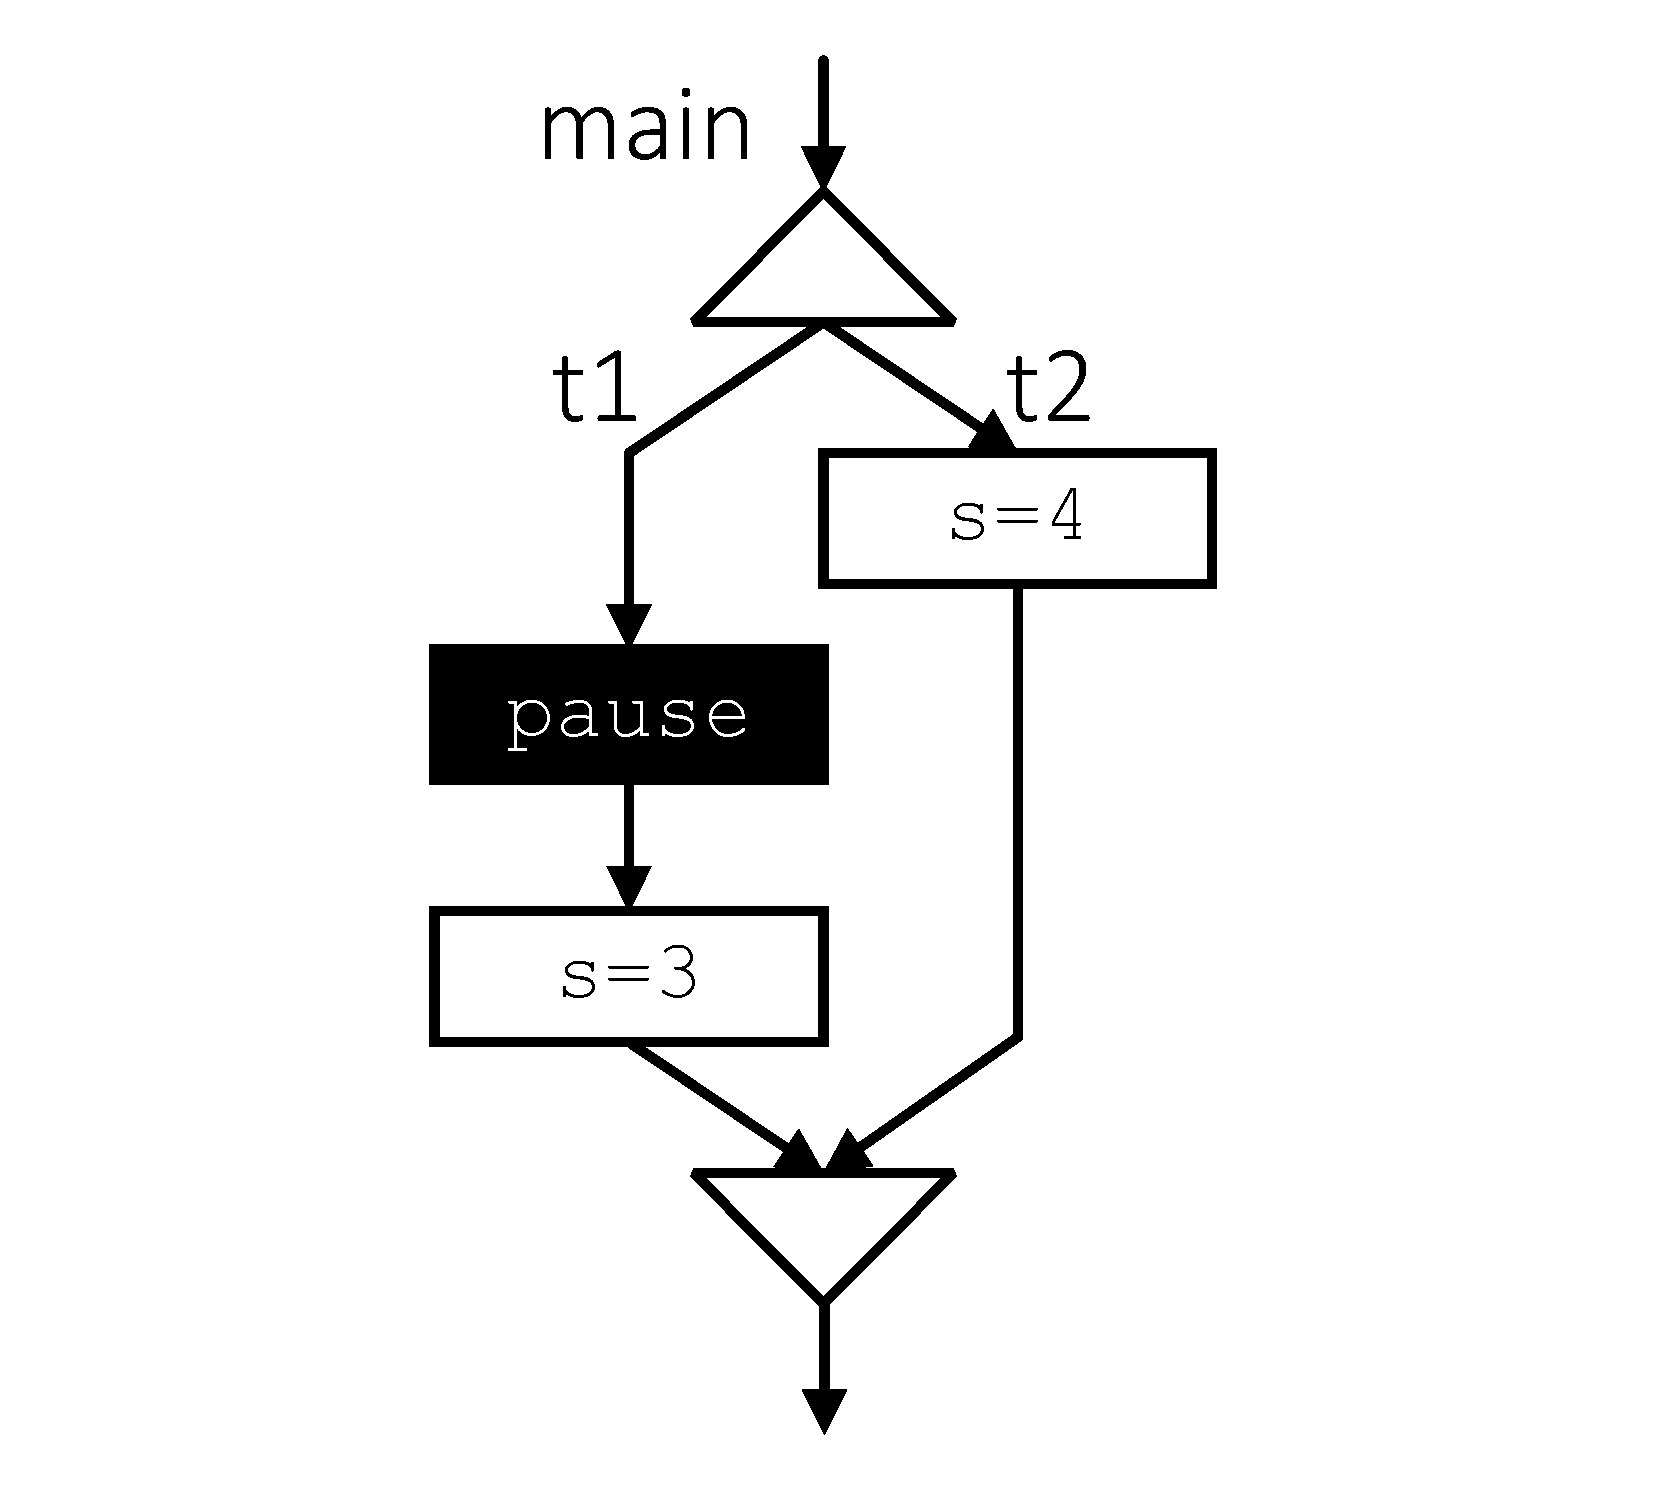
\includegraphics[width=\columnwidth]{program1_cfg}
			\label{fig:forec_semantics:program1_cfg}
		}
	\end{minipage}
	\hspace{0.1cm}

	\caption{Illustrative example one.}
\end{figure}

Before we apply the rewrite rules to the program, 
it is structurally translated into 
Figure~\ref{fig:forec_semantics:program1_kernel} 
(see the start of Section~\ref{sec:forec_semantics}).
Note that the semantic functions $\GetShared($\verb$main$$)$, 
$\GetShared($\verb$t1$$)$, $\GetShared($\verb$t2$$)$ 
and $\GetShared(\Global)$ all return $\lbrace$\verb$s$$\rbrace$.
The set of preemption statuses \Abort{} is initially $\emptyset$.
The program's environment \Environment{} and its derivatives 
are defined in Figure~\ref{figure:forec_program_2}.
\newline

\begin{figure}
	\centering
	$$\begin{array}{l l l}
		\Environment		&=& \left \lbrace
									\Global \to \lbrace s \to (0, \texttt{pre}) \rbrace
								\right \rbrace		\\
		\Environment^1		&=& \left \lbrace
									\Global \to \lbrace s \to (0, \texttt{pre}) \rbrace,
									main \to \lbrace s \to (0, \texttt{pre}) \rbrace
								\right \rbrace		\\
		\Environment^2		&=& \left \lbrace
									\Global \to \lbrace s \to (0, \texttt{pre}) \rbrace,
									main \to \lbrace s \to (0, \texttt{pre}) \rbrace,
									t1 \to \lbrace s \to (0, \texttt{pre}) \rbrace
								\right \rbrace		\\
		\Environment^3		&=& \left \lbrace
									\Global \to \lbrace s \to (0, \texttt{pre}) \rbrace,
									main \to \lbrace s \to (0, \texttt{pre}) \rbrace,
									t2 \to \lbrace s \to (0, \texttt{pre}) \rbrace
								\right \rbrace		\\
		\Environment^4		&=& \left \lbrace
									\Global \to \lbrace s \to (0, \texttt{pre}) \rbrace,
									main \to \lbrace s \to (0, \texttt{pre}) \rbrace,
									t1 \to \lbrace s \to (0, \texttt{pre}) \rbrace,
									t2 \to \lbrace s \to (0, \texttt{pre}) \rbrace
								\right \rbrace		\\
		\Environment^5		&=& \left \lbrace
									\Global \to \lbrace s \to (0, \texttt{pre}) \rbrace,
									main \to \lbrace s \to (0, \texttt{pre}) \rbrace,
									t1 \to \lbrace s \to (0, \texttt{pre}) \rbrace,
									t2 \to \lbrace s \to (4, \texttt{mod}) \rbrace
								\right \rbrace		\\
		\Environment^6		&=& \left \lbrace
									\Global \to \lbrace s \to (0, \texttt{pre}) \rbrace,
									main \to \lbrace s \to (4, \texttt{cmb}) \rbrace
								\right \rbrace		\\
		\Environment^7		&=& \left \lbrace
									\Global \to \lbrace s \to (4, \texttt{pre}) \rbrace
								\right \rbrace		\\
		\\
		\Environment^8		&=& \left \lbrace
									\Global \to \lbrace s \to (4, \texttt{pre}) \rbrace,
									t1 \to \lbrace s \to (4, \texttt{pre}) \rbrace
								\right \rbrace		\\
		\Environment^9		&=& \left \lbrace
									\Global \to \lbrace s \to (4, \texttt{pre}) \rbrace,
									t1 \to \lbrace s \to (3, \texttt{mod}) \rbrace
								\right \rbrace		\\
		\Environment^{10}	&=& \left \lbrace
									\Global \to \lbrace s \to (4, \texttt{pre}) \rbrace,
									main \to \lbrace s \to (3, \texttt{cmb}) \rbrace
								\right \rbrace		\\
		\Environment^{11}	&=& \left \lbrace
									\Global \to \lbrace s \to (3, \texttt{pre}) \rbrace
								\right \rbrace
	\end{array}$$
	
	\caption{Initial program environment and its derivatives.}
	\label{figure:forec_program_2}
\end{figure}

\noindent
\textbf{Step 1:}
Start the tick by applying the (\ref{forec:seq-right}) and
(\ref{forec:copy}) rules. 
\begin{prooftree}
			\AxiomC{}
		\LeftLabel{(\ref{forec:copy})}
		\UnaryInfC{$\langle \Environment, \Abort \rangle ~ \texttt{main:copy}
						\xrightarrow[~~\Input~~]{0} 
					\langle \Environment^1, \Abort \rangle ~ \texttt{main:}$}
	\LeftLabel{(\ref{forec:seq-right})}
	\UnaryInfC{$\begin{array}{l}
					\langle \Environment, \Abort \rangle ~ \texttt{main:copy;par(t1:\{copy;}	\\
					\texttt{pause;s=3;\},t2:\{copy;s=4;\})}
				\end{array}
					\xrightarrow[~~\Input~~]{\bot} 
				\begin{array}{l}
					\langle \Environment^1, \Abort \rangle ~ \texttt{main:par(t1:\{copy;}			\\
					\texttt{pause;s=3;\},t2:\{copy;s=4;\})}
				\end{array}$}
\end{prooftree}

\noindent
\textbf{Step 2:}
Both threads of the \texttt{par} execute sequential statements.
Apply the (\ref{forec:par-1}) rule. Additionally, apply the
(\ref{forec:seq-right}) and (\ref{forec:copy}) rules to both
threads. The environments of both threads, $\Environment^2$
and $\Environment^3$, are aggregated into $\Environment^4$.
\begin{prooftree}
				\AxiomC{}
			\LeftLabel{(\ref{forec:copy})}
			\UnaryInfC{$\langle \Environment^1, \Abort \rangle ~ \texttt{t1:copy}
							\xrightarrow[~~\Input~~]{0} 
						\langle \Environment^2, \Abort \rangle ~ \texttt{t1:}$}
		\LeftLabel{(\ref{forec:seq-right})}
		\UnaryInfC{$\begin{array}{l}
						\langle \Environment^1, \Abort \rangle ~ \texttt{t1:copy;}			\\
						\texttt{pause;s=3}
					\end{array}
						\xrightarrow[~~\Input~~]{\bot} 
					\begin{array}{l}
						\langle \Environment^2, \Abort \rangle ~ \texttt{t1:}				\\
						\texttt{pause;s=3}
					\end{array}$}
		%
				\AxiomC{}
			\UnaryInfC{$\langle \Environment^1, \Abort \rangle ~ \texttt{t2:copy}
							\xrightarrow[~~\Input~~]{0} 
						\langle \Environment^3, \Abort \rangle ~ \texttt{t2:}$}
		\UnaryInfC{$\begin{array}{l}
						\langle \Environment^1, \Abort \rangle ~ \texttt{t2:}					\\
						\texttt{copy;s=4;}
					\end{array}
						\xrightarrow[~~\Input~~]{\bot}
					\begin{array}{l}
						\langle \Environment^3, \Abort \rangle ~ \texttt{t2:}				\\
						\texttt{~~~~~~~s=4;}
					\end{array}$}
	%	
	\LeftLabel{(\ref{forec:par-1})}
	\BinaryInfC{$\begin{array}{l}
					\langle \Environment^1, \Abort \rangle ~ \texttt{main:par(t1:\{copy;}		\\
					\texttt{pause;s=3;\},t2:\{copy;s=4;\})}
				\end{array}
					\xrightarrow[~~\Input~~]{\bot} 
				\begin{array}{l}
					\langle \Environment^4, \Abort \rangle ~ \texttt{main:par(t1:\{pause;}		\\
					\texttt{~~~~~~~s=3;\},t2:\{s=4;\})}
				\end{array}$}
\end{prooftree}

\noindent
\textbf{Step 3:}
Apply the (\ref{forec:tick}) and (\ref{forec:par-7}) rules.
Additionally, apply the (\ref{forec:seq-left}) and
(\ref{forec:pause}) rules to the first thread and the
(\ref{forec:assign-shared}) rule to the second thread.
\textbf{The program completes the tick.} Note that when the
(\ref{forec:par-7}) rule is applied, the aggregated
environment is the same as~$\Environment^5$, which is then
combined to be $\Environment^6$. When the (\ref{forec:tick})
rule is applied, $\Environment^6$ is resynchronized to be
$\Environment^7$.
\begin{prooftree}
					\AxiomC{}
				\LeftLabel{(\ref{forec:pause})}
				\UnaryInfC{$\begin{array}{l}
								\langle \Environment^4, \Abort \rangle ~ \texttt{t1:}		\\
								\texttt{~~~~pause}
							\end{array}
								\xrightarrow[~~\Input~~]{1}
							\begin{array}{l}
								\langle \Environment^4, \Abort \rangle ~ \texttt{t1:}		\\
								\texttt{~~~~~copy}
							\end{array}$}
			\LeftLabel{(\ref{forec:seq-left})}
			\UnaryInfC{$\begin{array}{l}
							\langle \Environment^4, \Abort \rangle ~ \texttt{t1:}			\\
							\texttt{pause;s=3}
						\end{array}
							\xrightarrow[~~\Input~~]{1}
						\begin{array}{l}
							\langle \Environment^4, \Abort \rangle ~ \texttt{t1:}			\\
							\texttt{copy;s=3}
						\end{array}$}
			%
				\AxiomC{$s \in \lbrace s \rbrace$}
			\LeftLabel{(\ref{forec:assign-shared})}
			\UnaryInfC{$\begin{array}{l}
							\langle \Environment^4, \Abort \rangle ~ \texttt{t2:}			\\
							\texttt{~~~~~~s=4;}
						\end{array}
							\xrightarrow[~~\Input~~]{0} 
						\langle \Environment^5, \Abort \rangle ~ \texttt{t2:}$}
		%
		\LeftLabel{(\ref{forec:par-7})}
		\BinaryInfC{$\begin{array}{l}
						\langle \Environment^4, \Abort \rangle ~ \texttt{main:par(t1:\{pause;}	\\
						\texttt{~~~~~~~s=3;\},t2:\{s=4;\})}
					\end{array}
						\xrightarrow[~~\Input~~]{1} 
					\begin{array}{l}
						\langle \Environment^6, \Abort \rangle ~ \texttt{main:par(t1:\{copy;}	\\
						\texttt{~~~~~~~s=3;\},t2:nop)}
					\end{array}$}
	\LeftLabel{(\ref{forec:tick})}
	\UnaryInfC{$\begin{array}{l}
					\langle \Environment^4, \Abort \rangle ~ \texttt{main:par(t1:\{pause;}		\\
					\texttt{~~~~~~~s=3;\},t2:\{s=4;\})}
				\end{array}
					\xrightarrow[~~\Input~~]{1} 
				\begin{array}{l}
					\langle \Environment^7, \Abort \rangle ~ \texttt{main:par(t1:\{copy;}		\\
					\texttt{~~~~~~~s=3;\},t2:nop)}
				\end{array}$}
\end{prooftree}

\noindent
\textbf{Step 4:}
Start the next tick by applying the (\ref{forec:par-3})
rule. Additionally, apply the (\ref{forec:seq-right}) and
(\ref{forec:copy}) rules to the first thread and the
(\ref{forec:nop}) rule to the second thread.
\begin{prooftree}
				\AxiomC{}
			\LeftLabel{(\ref{forec:copy})}
			\UnaryInfC{$\langle \Environment^7, \Abort \rangle ~ \texttt{t1:copy}
							\xrightarrow[~~\Input~~]{0} 
						\langle \Environment^8, \Abort \rangle ~ \texttt{t1:}$}
		\LeftLabel{(\ref{forec:seq-right})}
		\UnaryInfC{$\begin{array}{l}
						\langle \Environment^7, \Abort \rangle ~ \texttt{t1:}				\\
						\texttt{copy;s=3}
					\end{array}
						\xrightarrow[~~\Input~~]{\bot}
					\langle \Environment^8, \Abort \rangle ~ \texttt{t1:s=3}$}
		%
			\AxiomC{}
		\LeftLabel{(\ref{forec:nop})}
		\UnaryInfC{$\begin{array}{l}
						\langle \Environment^7, \Abort \rangle ~ \texttt{t2:}				\\
						\texttt{~~~~~~~nop}
					\end{array}
						\xrightarrow[~~\Input~~]{0} 
					\langle \Environment^7, \Abort \rangle ~ \texttt{t2:}$}
	%
	\LeftLabel{(\ref{forec:par-3})}
	\BinaryInfC{$\begin{array}{l}
					\langle \Environment^7, \Abort \rangle ~ \texttt{main:par(t1:\{copy;}	\\
					\texttt{~~~~~~~s=3;\},t2:nop)}
				\end{array}
					\xrightarrow[~~\Input~~]{\bot} 
				\langle \Environment^8, \Abort \rangle ~ \texttt{main:par(t1:\{s=3;\},t2:nop)}$}
\end{prooftree}

\noindent
\textbf{Step 5:}
Apply the (\ref{forec:par-5}) rule. Additionally, apply the
(\ref{forec:assign-shared}) rule to the first thread and the
(\ref{forec:nop}) rule to the second thread. Note that when
the (\ref{forec:par-5}) rule is applied, the aggregated
environment is the same as $\Environment^9$, which is then
combined to be~$\Environment^{10}$.
\begin{prooftree}
			\AxiomC{$s \in \lbrace s \rbrace$}
		\LeftLabel{(\ref{forec:assign-shared})}
		\UnaryInfC{$\begin{array}{l}
						\langle \Environment^8, \Abort \rangle ~ \texttt{t1:}				\\
						\texttt{~~~~~~s=3}
					\end{array}
						\xrightarrow[~~\Input~~]{0} 
					\langle \Environment^9, \Abort \rangle ~ \texttt{t1:}$}
	%
			\AxiomC{}
		\LeftLabel{(\ref{forec:nop})}
		\UnaryInfC{$\begin{array}{l}
						\langle \Environment^8, \Abort \rangle ~ \texttt{t2:}				\\
						\texttt{~~~~~~nop}
					\end{array}
						\xrightarrow[~~\Input~~]{0} 
					\langle \Environment^8, \Abort \rangle ~ \texttt{t2:}$}
	%
	\LeftLabel{(\ref{forec:par-5})}
	\BinaryInfC{$\langle \Environment^8, \Abort \rangle ~ \texttt{main:par(t1:\{s=3;\},t2:nop)}
					\xrightarrow[~~\Input~~]{\bot} 
				\langle \Environment^{10}, \Abort \rangle ~ \texttt{main:copy}$}
\end{prooftree}

\noindent
\textbf{Step 6:}
Apply the (\ref{forec:tick}) and (\ref{forec:copy}) rules.
The environment $\Environment^{10}$ is resynchronized to be
$\Environment^{11}$. \textbf{The tick ends and the program terminates.}
\begin{prooftree}
			\AxiomC{}
		\LeftLabel{(\ref{forec:copy})}
		\UnaryInfC{$\langle \Environment^{10}, \Abort \rangle ~ \texttt{main:copy}
						\xrightarrow[~~\Input~~]{0} 
					\langle \Environment^{10}, \Abort \rangle ~ \texttt{main:}$}
	\LeftLabel{(\ref{forec:tick})}
	\UnaryInfC{$\langle \Environment^{10}, \Abort \rangle ~ \texttt{main:copy}
					\xrightarrow[~~\Input~~]{0} 
				\langle \Environment^{11}, \Abort \rangle ~ \texttt{main:}$}
\end{prooftree}

\subsubsection{Example Two}
The second program illustrates the preemption by using an 
immediate weak \verb$abort$ statement. 
Figure~\ref{fig:forec_semantics:program2} presents
the ForeC program and Figure~\ref{fig:forec_semantics:program2_cfg}
illustrates the program's control-flow. In 
Figure~\ref{fig:forec_semantics:program2_cfg}, the
pair of decorated diamonds represents the scope of the 
\verb$abort$ body.

In the program's first tick, the \verb$main$ thread
reaches the immediate and weak \verb$abort$ and immediately
evaluates the preemption condition \verb$(x==1)$. The
condition evaluates to \emph{true} and the preemption is 
triggered. Since the \verb$abort$ is weak, the preemption
is taken only when execution reaches the \verb$pause$, after
the variable \verb$x$ has been incremented. The 
\verb$abort$ terminates and, as a result, the \verb$main$
thread terminates. The first tick ends.

\begin{figure}
	\centering
	
	\hfill
	\begin{minipage}{0.43\columnwidth}
		\subfloat[ForeC program.] {
			\lstinputlisting[style=full]{./code/forec/illustration/program2.forec}
			\label{fig:forec_semantics:program2}
		}

		\subfloat[Translated kernel program.] {
			\lstinputlisting[style=full]{./code/forec/illustration/program2_kernel.forec}
			\label{fig:forec_semantics:program2_kernel}
		}
	\end{minipage}
	\hspace{0.5cm}
	\begin{minipage}{0.28\columnwidth}
		\subfloat[Control-flow graph.] {
			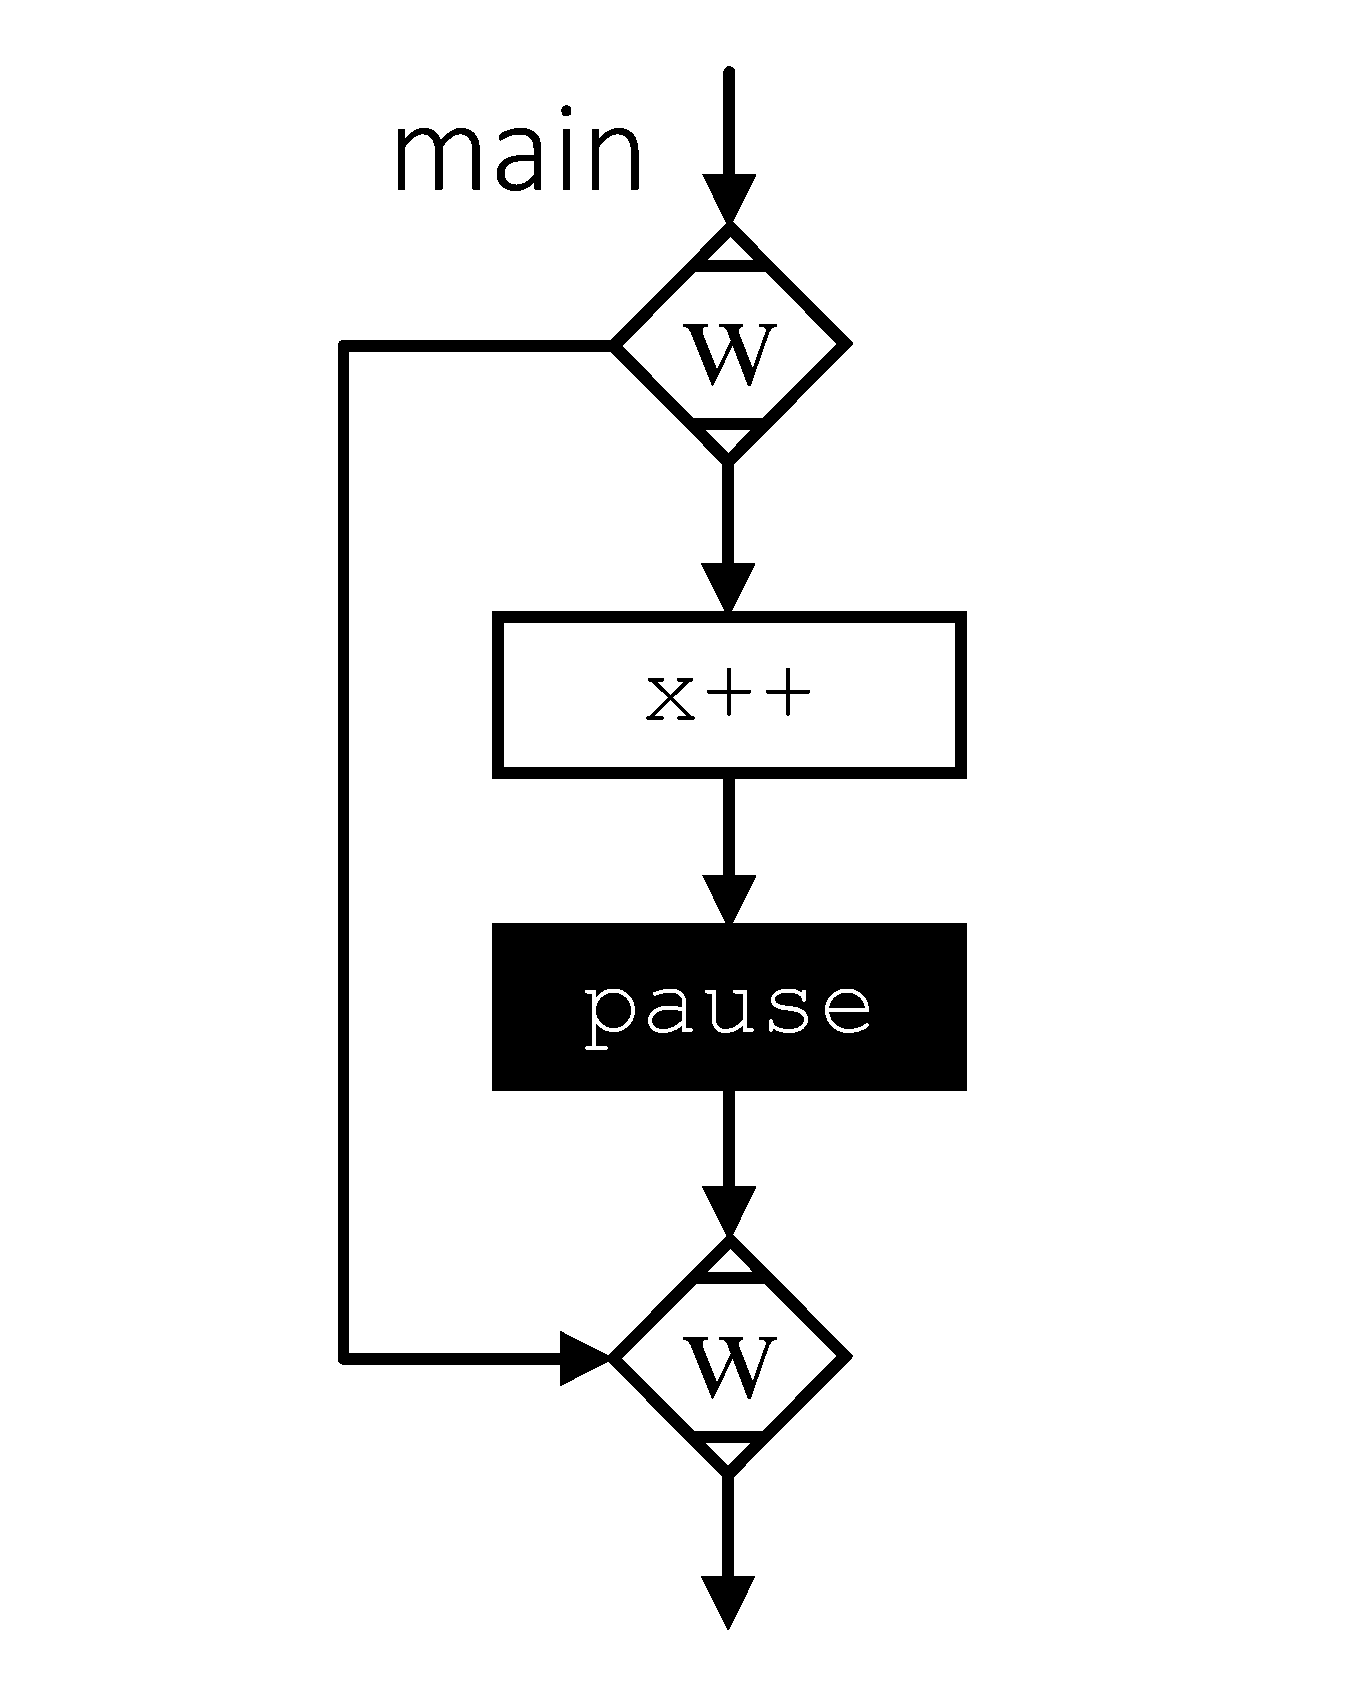
\includegraphics[width=\columnwidth]{program2_cfg}
			\label{fig:forec_semantics:program2_cfg}
		}
	\end{minipage}
	\hspace{1.5cm}

	\caption{Illustrative example two.}
\end{figure}

Before we apply the rewrite rules to the program, 
it is structurally translated into 
Figure~\ref{fig:forec_semantics:program2_kernel} 
(see the start of Section~\ref{sec:forec_semantics}).
The \verb$copy$ kernel statement is not inserted into
the program because no shared variables are used.
Note that the semantic functions $\GetShared($\verb$main$$)$ 
and $\GetShared(\Global)$ all return $\emptyset$.
The program's environment \Environment{}, preemption statuses \Abort{},
and their derivatives are defined in Figure~\ref{figure:forec_program_3}.
\newline

\begin{figure}
	\centering
	$$\begin{array}{l l l l l l}
		\Environment		&=& \left \lbrace
									\Global \to \lbrace x \to (1, \texttt{pvt}) \rbrace
								\right \rbrace	& \qquad 
		\Abort				&=& \lbrace a1 \rbrace			\\
		\Environment^1		&=& \left \lbrace
									\Global \to \lbrace x \to (2, \texttt{pvt}) \rbrace
								\right \rbrace	& \qquad 
		\Abort^1			&=& \lbrace a1 \to 1 \rbrace	\\
		& & & \qquad 
		\Abort^2			&=& \lbrace a1 \to 0 \rbrace
	\end{array}$$
	
	\caption{Initial program state and its derivatives.}
	\label{figure:forec_program_3}
\end{figure}

\noindent
\textbf{Step 1:} Start the tick by applying the
(\ref{forec:seq-right}) and (\ref{forec:status}) rules. Note
that the \verb$abort$'s preemption is triggered because the
condition \verb$x==1$ evaluates to $1$.
\begin{prooftree}
			\AxiomC{}
		\LeftLabel{(\ref{forec:status})}
		\UnaryInfC{$\langle \Environment, \Abort \rangle ~ \texttt{main: status(a1,x==1)}
						\xrightarrow[~~\Input~~]{0} 
					\langle \Environment, \Abort^1 \rangle ~ \texttt{main:}$}
	\LeftLabel{(\ref{forec:seq-right})}
	\UnaryInfC{$\begin{array}{l}
					\langle \Environment, \Abort \rangle ~ \texttt{main:status(a1,x==1);}		\\
					\texttt{weak~abort(a1,\{x++;pause;\})}
				\end{array}
					\xrightarrow[~~\Input~~]{\bot} 
				\begin{array}{l}
					\langle \Environment, \Abort^1 \rangle ~ \texttt{main:weak~abort}		\\
					\texttt{(a1,\{x++;pause;\})}
				\end{array}$}
\end{prooftree}

\noindent
\textbf{Step 2:}
Apply the (\ref{forec:abort-4}), (\ref{forec:seq-right}), and (\ref{forec:assign-private}) rules.
\begin{prooftree}
				\AxiomC{$x \notin \emptyset$}
			\LeftLabel{(\ref{forec:assign-private})}
			\UnaryInfC{$\langle \Environment, \Abort^1 \rangle ~ \texttt{main:x++}
							\xrightarrow[~~\Input~~]{0} 
						\langle \Environment^1, \Abort^1 \rangle ~ \texttt{main:}$}
		\LeftLabel{(\ref{forec:seq-right})}
		\UnaryInfC{$\langle \Environment, \Abort^1 \rangle ~ \texttt{main:x++;pause}
						\xrightarrow[~~\Input~~]{\bot} 
					\langle \Environment^1, \Abort^1 \rangle ~ \texttt{main:pause}$}
	\LeftLabel{(\ref{forec:abort-4})}\RightLabel{$(\Abort^1[a1] \neq 0)$}
	\UnaryInfC{$\begin{array}{l}
					\langle \Environment, \Abort^1 \rangle ~ \texttt{main:weak~abort}		\\
					\texttt{(a1,\{x++;pause;\})}
				\end{array}
					\xrightarrow[~~\Input~~]{\bot} 
				\begin{array}{l}
					\langle \Environment^1, \Abort^1 \rangle ~ \texttt{main:weak~abort}		\\
					\texttt{(a1,\{pause;\})}
				\end{array}$}
\end{prooftree}

\noindent
\textbf{Step 3:}
Apply the (\ref{forec:abort-5}) and (\ref{forec:pause}) 
rules. Note that the preemption is taken because the \verb$abort$'s
body has reached a \verb$pause$.
\begin{prooftree}
			\AxiomC{}
		\LeftLabel{(\ref{forec:pause}) }
		\UnaryInfC{$\langle \Environment^1, \Abort^1 \rangle ~ \texttt{main:pause}
						\xrightarrow[~~\Input~~]{1} 
					\langle \Environment^1, \Abort^1 \rangle ~ \texttt{main:copy}$}
	\LeftLabel{(\ref{forec:abort-5})}\RightLabel{$(\Abort^1[a1] \neq 0)$}
	\UnaryInfC{$\langle \Environment^1, \Abort^1 \rangle ~ \texttt{main:weak~abort(a1,\{pause;\})}
					\xrightarrow[~~\Input~~]{\bot} 
				\langle \Environment^1, \Abort^1 \rangle ~ \texttt{main:copy}$}
\end{prooftree}

\noindent
\textbf{Step 4:}
Apply the (\ref{forec:tick}) and (\ref{forec:copy}) 
rules. The preemption statuses in $\Abort^1$ are
updated to be~$\Abort^2$.
\textbf{The tick ends and the program terminates.}
\begin{prooftree}
			\AxiomC{}
		\LeftLabel{(\ref{forec:copy})}
		\UnaryInfC{$\langle \Environment^1, \Abort^1 \rangle ~ \texttt{main:copy}
						\xrightarrow[~~\Input~~]{0} 
					\langle \Environment^1, \Abort^1 \rangle ~ \texttt{main:}$}
	\LeftLabel{(\ref{forec:tick})}
	\UnaryInfC{$\langle \Environment^1, \Abort^1 \rangle ~ \texttt{main:copy}
					\xrightarrow[~~\Input~~]{0} 
				\langle \Environment^1, \Abort^2 \rangle ~ \texttt{main:}$}
\end{prooftree}


%\section{Proofs}
\subsection{Definitions and Proofs}
\label{sec:forec_proofs}

%\subsection{Reactivity and Determinism of ForeC Programs}
The semantics of the ForeC kernel constructs (Section~\ref{sec:forec_semantics:sos}) 
can be used to
formally prove two desirable properties of safety-critical
programs, called \emph{reactivity} and
\emph{determinism}~\cite{Maraninchi92,Tardieu07}. A program
is reactive if it always responds to changes in the
environment, i.e., does not deadlock and produces outputs. 
A program is deterministic if, for a given set of inputs from the 
environment, there is at most one set of outputs produced by the 
programs. In terms of semantic derivation rules, a program is 
deterministic if there is at most one derivation tree in
response to the environment. The
definitions for reactivity and determinism are normally
based on a program's tick, which is a sequence of
transitions. Because the state of a ForeC program depends on
the initial valuations of its variables, we define a stronger notion
of reactivity and determinism based on program transitions. 

%\begin{definition}
%	\label{def:reaction}
%	A completed \emph{\textbf{reaction}} of program $\thread{}:\body{}$ 
%	in a tick is denoted by:
%	\begin{equation*}
%		\langle \StateP \rangle ~ \thread{}:\body{} 
%			\xRightarrow[~~\Input~~]{k \in \{0, 1\}} 
%		\langle \StateP' \rangle ~ \thread{}:\body{}'
%	\end{equation*}
%	if there exists a sequence of rewrites with $k = \bot$
%	that ends in a rewrite with $k \in \{0, 1\}$:
%	\begin{equation*}
%		\langle \StateP \rangle ~ \thread{}:\body{} 
%			\xrightarrow[~~\Input~~]{\bot}
%		\langle \StateP^1 \rangle ~ \thread{}:\body{1}
%			\xrightarrow[~~\Input~~]{\bot}
%			\dotsb
%			\xrightarrow[~~\Input~~]{\bot}
%		\langle \StateP^n \rangle ~ \thread{}:\body{n}
%			\xrightarrow[~~\Input~~]{k \in \{0, 1\}} 
%		\langle \StateP' \rangle ~ \thread{}:\body{}'
%	\end{equation*}
%\end{definition}

\begin{definition}
	\label{def:reactive}
	A program $\thread{}:\body{}$ is \emph{\textbf{reactive}} if,  
	in any state \StateP{}, for any input configuration \Input{}, 
	there exists at least one transition
	(i.e., the program never deadlocks):
	\begin{equation*}
		\forall \StateP, \Input: \quad
		\exists \StateP', \body{}', k
		\quad \text{such that} \quad
		\langle \StateP \rangle ~ \thread{}:\body{} 
			\xrightarrow[~~\Input~~]{k} 
		\langle \StateP' \rangle ~ \thread{}:\body{}'
	\end{equation*}
\end{definition}

\begin{theorem}
	\label{thm:reactive}
	All ForeC programs are \emph{\textbf{reactive}}.
\end{theorem}
\begin{proof}
	The proof can be shown by structural induction on $\thread{}:\body{}$.
	
	\textbf{Base cases:}
	The (\ref{forec:nop}), (\ref{forec:copy}), (\ref{forec:pause}), (\ref{forec:status}),
	(\ref{forec:assign-shared}), (\ref{forec:assign-private}), (\ref{forec:if-then}), 
	(\ref{forec:if-else}), (\ref{forec:loop-then}), and (\ref{forec:loop-else})
	rules imply that the following kernel constructs have at least one transition:
	\begin{align*}
		\langle \StateP \rangle ~ \thread{}:\mathtt{nop}
			\xrightarrow[~~\Input~~]{0}& 
		\langle \StateP \rangle ~ \thread{}:									\\
		%
		\langle \StateP \rangle ~ \thread{}:\mathtt{copy}
			\xrightarrow[~~\Input~~]{0}& 
		\langle \StateP' \rangle ~ \thread{}:									\\
		%
		\langle \StateP \rangle ~ \thread{}:\mathtt{pause}
			\xrightarrow[~~\Input~~]{1}& 
		\langle \StateP \rangle ~ \thread{}:\mathtt{copy}						\\
		%
		\langle \StateP \rangle ~ \thread{}:\mathtt{status}(a, \expression)
			\xrightarrow[~~\Input~~]{0}& 
		\langle \StateP' \rangle ~ \thread{}:									\\
		%
		\langle \StateP \rangle ~ \thread{}:\var \mathtt{=} \expression
			\xrightarrow[~~\Input~~]{0}& 
		\langle \StateP' \rangle ~ \thread{}:									\\
		%
		\langle \StateP \rangle ~ \thread{}:\mathtt{if}~(\expression)~\body{1}~\mathtt{else}~\body{2}
			\xrightarrow[~~\Input~~]{\bot} 
		\langle \StateP \rangle ~ \thread{}:\body{1}
		\quad \text{or} \quad &
		\langle \StateP \rangle ~ \thread{}:\mathtt{if}~(\expression)~\body{1}~\mathtt{else}~\body{2}
			\xrightarrow[~~\Input~~]{\bot} 
		\langle \StateP \rangle ~ \thread{}:\body{2}							\\
		%
		\langle \StateP \rangle ~ \thread{}:\mathtt{while}~(\expression)~\body{}
			\xrightarrow[~~\Input~~]{\bot}
		\langle \StateP \rangle ~ \thread{}:\body{};~\mathtt{while}~(\expression)~\body{}
		\quad \text{or} \quad &
		\langle \StateP \rangle ~ \thread{}:\mathtt{while}~(\expression)~\body{}
			\xrightarrow[~~\Input~~]{0}
		\langle \StateP \rangle ~ \thread{}:
	\end{align*}
	%Note that the assignment, \verb$if$--\verb$else$, and \verb$while$ kernel constructs 
%	are each described by a pair of rewrite rules with complementary premises that 
%	do not depend on other transitions. 
%	The premises are complementary in the sense that, if the premise of one rule is \emph{true}, 
%	then the premise of the other rule must be \emph{false}, and vice versa.
	
	\textbf{Induction step:}
	The sequence operator (\verb$;$), \verb$abort$, and \verb$par$ 
	kernel statements allow the composition of kernel constructs.
	For some $\thread{1}:\body{1}$ and $\thread{2}:\body{2}$ that 
	are arbitrary compositions of kernel constructs, assume the induction hypotheses 
	that they each have at least one transition:
	\begin{align*}
		\exists \StateP_1', \StateP_2', \body{1}', \body{2}', k_1, k_2
		\quad \text{such that} \quad
		\tag{H1}
		\label{forec_proofs:H1}
		\langle \StateP_1 \rangle ~ \thread{1}:\body{1}
		&	\xrightarrow[~~\Input~~]{k_1} 
		\langle \StateP_1' \rangle ~ \thread{1}:\body{1}'						\\
		%
		\tag{H2}
		\label{forec_proofs:H2}
		\langle \StateP_2 \rangle ~ \thread{2}:\body{2}
		&	\xrightarrow[~~\Input~~]{k_2} 
		\langle \StateP_2' \rangle ~ \thread{2}:\body{2}'
	\end{align*}
	Next, we show that the remaining sequence operator (\verb$;$), 
	\verb$abort$, and \verb$par$ kernel statements have at least one transition.
	\begin{enumerate}
		\item Consider $\thread{1}: \body{1}\mathtt{;}~\body{2}$. 
			  Due to the induction hypotheses, the table below shows that at least one
			  sequence rule can be applied to all possible completion codes $k_1$
			  of the first program fragment \body{1}. Note that the sequence rules
			  do not consider the completion code $k_2$ of the second program fragment 
			  \body{2}:
			  \begin{center}
			  	\def\arraystretch{1.3}
				\begin{tabular}{| c | c | c |}
					\hline
					\multicolumn{3}{| c |}{\boldmath$k_1$}										\\ 
					~~~~~\textbf{0}~~~~~	& ~~~~~\textbf{1}~~~~~	& ~~~~~\boldmath$\bot$~~~~~	\\ \hline 
					(\ref{forec:seq-right})	& \multicolumn{2}{c|}{(\ref{forec:seq-left})}		\\
					\hline
				\end{tabular}
			  \end{center}
			  If $k_1 = 0$ and the premise is true by the induction 
			  hypothesis~(\ref{forec_proofs:H1}), then from the (\ref{forec:seq-right}) 
			  rule we have:
			  \begin{prooftree}
			  			\AxiomC{$\langle \StateP_1 \rangle ~ \thread{1}:\body{1}
									\xrightarrow[~~\Input~~]{k_1 = 0}
								\langle \StateP_1' \rangle ~ \thread{1}:$}
					\LeftLabel{(\ref{forec:seq-right})}
					\UnaryInfC{$\langle \StateP_1 \rangle ~ \thread{1}: \body{1}\mathtt{;}~\body{2}
									\xrightarrow[~~\Input~~]{\bot} 
								\langle \StateP_1' \rangle ~ \thread{1}: \body{2}$}
			  \end{prooftree}
			  If $k_1 \in \lbrace 1, \bot \rbrace$ and the premise is true by the 
			  induction hypothesis~(\ref{forec_proofs:H1}), then from the (\ref{forec:seq-left}) 
			  rule we have:
			  \begin{prooftree}
			  			\AxiomC{$\langle \StateP_1 \rangle ~ \thread{1}:\body{1}
									\xrightarrow[~~\Input~~]{k_1 \in \lbrace 1, \bot \rbrace}
								\langle \StateP_1' \rangle ~ \thread{1}:\body{1}'$}
					\LeftLabel{(\ref{forec:seq-left})}
					\UnaryInfC{$\langle \StateP_1 \rangle ~ \thread{1}: \body{1}\mathtt{;}~\body{2}
									\xrightarrow[~~\Input~~]{k_1} 
								\langle \StateP_1' \rangle ~ \thread{1}: \body{1}'\mathtt{;}~\body{2}$}
			  \end{prooftree}
			  Thus, any sequential composition of reactive programs has at least one 
			  transition and is, therefore, reactive.
			  
		\item Consider $\thread{1}: \mathtt{weak}?~\mathtt{abort}(a_1, \body{1})$. 
			  Due to the induction hypotheses, the table below shows that at least one 
			  \verb$abort$ rule can be applied to every combination of $k_1$ and 
			  preemption status $\Abort[a_1]$:
			  \begin{center}
			  	\def\arraystretch{1.3}
				\begin{tabular}{| c c | c | c | c | c | c | c |}
					\cline{3-8}
					\multicolumn{2}{c|}{}										& \multicolumn{3}{c |}{\textbf{Strong \texttt{abort},} \boldmath$k_1$} 								& \multicolumn{3}{c |}{\textbf{Weak \texttt{abort},} \boldmath$k_1$}	\\ 
					\multicolumn{2}{c|}{}										& ~~~~~\textbf{0}~~~~~	& ~~~~~\textbf{1}~~~~~							& ~~~~~\boldmath$\bot$~~~~~	& ~~~~~\textbf{0}~~~~~	& ~~~~~\textbf{1}~~~~~	& \boldmath$\bot$		\\ \hline 
					\multirow{2}{*}{\boldmath$\Abort[a_1]$}	& \boldmath$= 0$	& (\ref{forec:abort-2})	& \multicolumn{2}{c|}{(\ref{forec:abort-1})}								& (\ref{forec:abort-2})	& \multicolumn{2}{c|}{(\ref{forec:abort-1})}	\\ \cline{2-8}
															& \boldmath$\neq 0$	& \multicolumn{3}{c|}{(\ref{forec:abort-6})}														& (\ref{forec:abort-3})	& (\ref{forec:abort-5})	& (\ref{forec:abort-4})	\\
					\hline
				\end{tabular}
			  \end{center}
			  For example, if $k_1 = 0$ and $\Abort[a_1] = 0$ and the premise is true by 
			  the induction hypothesis~(\ref{forec_proofs:H1}), then from the (\ref{forec:abort-2}) rule
			  we have:
			  \begin{prooftree}
			  			\AxiomC{$\langle \StateP_1 \rangle ~ \thread{1}:\body{1}
									\xrightarrow[~~\Input~~]{k_1 = 0} 
								\langle \StateP_1' \rangle ~ \thread{1}:$}
					\LeftLabel{(\ref{forec:abort-2})}\RightLabel{$(\Abort[a_1] = 0)$}
					\UnaryInfC{$\langle \StateP_1 \rangle ~ \thread{1}: \mathtt{weak}?~\mathtt{abort}(a_1, \body{1})
									\xrightarrow[~~\Input~~]{0} 
								\langle \StateP_1' \rangle ~ \thread{1}:$}
			  \end{prooftree}
			  The other cases are similar. Thus, any preemptive composition of reactive programs 
			  has at least one transition and is, therefore, reactive.

		\item Consider $\thread{}:\mathtt{par}(\thread{1}:\body{1},~\thread{2}:\body{2})$.
			  Due to the induction hypotheses, the table below shows that at least one
			  \verb$par$ rule can be applied to every combination of $k_1$ and $k_2$:
			  \begin{center}
			  	\def\arraystretch{1.3}
				\begin{tabular}{| c c | c | c | c |}
					\cline{3-5}
					\multicolumn{2}{c|}{}				& \multicolumn{3}{c |}{\boldmath$k_2$}													\\ 
					\multicolumn{2}{c|}{}				& \textbf{0}			& \textbf{1}			& \boldmath$\bot$						\\ \hline 
									& \textbf{0}		& (\ref{forec:par-5})	& (\ref{forec:par-6})	& \multirow{2}{*}{(\ref{forec:par-2})}	\\ \cline{2-4}
					\boldmath$k_1$	& \textbf{1}		& (\ref{forec:par-7})	& (\ref{forec:par-4})	&										\\ \cline{2-5}
									& \boldmath$\bot$	& \multicolumn{2}{c|}{(\ref{forec:par-3})}		& (\ref{forec:par-1})					\\
					\hline
				\end{tabular}
			  \end{center}
			  For example, if $k_1 = 0$ and $k_2 = 0$ and the premise is true by 
			  the induction hypotheses~(\ref{forec_proofs:H1}) and (\ref{forec_proofs:H2}), 
			  then from the (\ref{forec:par-5}) rule we have:
			  \begin{prooftree}
			  			\AxiomC{$\langle \StateP \rangle ~ \thread{1}:\body{1}
									\xrightarrow[~~\Input~~]{k_1 = 0} 
								\langle \StateP_1' \rangle ~ \thread{1}:
								\qquad\qquad
								\langle \StateP \rangle ~ \thread{2}:\body{2}
									\xrightarrow[~~\Input~~]{k_2 = 0} 
								\langle \StateP_2' \rangle ~ \thread{2}:$}
					\LeftLabel{(\ref{forec:par-5})}
					\UnaryInfC{$\langle \StateP \rangle ~ \thread{}: \mathtt{par}(\thread{1}:\body{1},~\thread{2}:\body{2})
									\xrightarrow[~~\Input~~]{\bot} 
								\langle \StateP'' \rangle ~ \thread{}: \mathtt{copy}$}
			  \end{prooftree}
			  The other cases are similar. Thus, any parallel composition of reactive 
			  programs has at least one transition and is, therefore, reactive.
	\end{enumerate}
\end{proof}

\begin{definition}
	\label{def:deterministic}
	A program $\thread{}:\body{}$ is \emph{\textbf{deterministic}} if, 
	in any state \StateP{}, for any input configuration~\Input{}, there 
	exists at most one transition such that:
	\begin{align*}
		\forall \StateP, \Input: \quad
		\text{if} \quad
		\langle \StateP \rangle ~ \thread{}:\body{} 
		&	\xrightarrow[~~\Input~~]{k'} 
		\langle \StateP'~ \rangle ~ \thread{}:\body{}'	\\
		\text{and} \quad
		\langle \StateP \rangle ~ \thread{}:\body{} 
		&	\xrightarrow[~~\Input~~]{k''} 
		\langle \StateP'' \rangle ~ \thread{}:\body{}''
		\quad \text{then} \quad 
		\StateP' = \StateP'', ~ \body{}' = \body{}'', ~ k' = k''
	\end{align*}
\end{definition}
Only the rewrite rules of the \verb$par$ statement allow state 
\StateP{} to be changed in parallel by multiple transitions. The
(\ref{forec:par-1}) rule aggregates the changes into a
single state. The (\ref{forec:par-4}), (\ref{forec:par-5}),
(\ref{forec:par-6}), and (\ref{forec:par-7}) rules use the
semantic function $\Combine$ (Algorithm~\ref{algo:Combine})
to combine the copies in the aggregated state. The
(\ref{forec:par-2}) and (\ref{forec:par-3}) rules only allow
one of the changed states to take effect. Before proving
that all ForeC programs are deterministic, we prove that the
aggregation of states and the semantic function $\Combine$
are both deterministic. This is captured by
Lemmas~\ref{lem:aggregation} and \ref{lem:Combine} below
with the assumption that all the combine functions are
deterministic.

\begin{definition}
	\label{def:combine}
	A combine function $cf$ is any C function with two input
	values~$\val_1$ and $\val_2$ of identical type, which
	returns a value of the same type.
\end{definition}

\begin{hypothesis} 
	\label{hyp:combine}
	Each combine function $cf$ always returns the same value regardless
	of the current state, provided that the input values, $\val_1$
	and $\val_2$, are identical:
%
	\begin{align*}
		\forall \StateP, \StateP', \Input, \thread{},& \val_1, \val_2:	\\
		\qquad \qquad
		& \Eval(\StateP.\Environment, \Input, \thread{}, cf(\val_1, \val_2)) = \Eval(\StateP'.\Environment, \Input, \thread{}, cf(\val_1, \val_2))
	\end{align*}
%
	Because the combine functions are defined in~C, we require that the
	combine functions always terminate without error.\end{hypothesis}

\begin{lemma}
	\label{lem:aggregation}
	For any initial state\footnotemark[7] $\StateP = \langle \Environment, \Abort \rangle$, 
	let $\StateP' = \langle \Environment', \Abort' \rangle$ and 
	$\StateP'' = \langle \Environment'', \Abort'' \rangle$ be the states
	of two threads after their transition.
	If the threads can only change their own private variables and 
	copies of shared variables, then the aggregation of 
	$\StateP'$ and $\StateP''$ is \emph{\textbf{deterministic}} 
	if there exists only one aggregated state:
	\begin{align*}
		\forall \StateP = \langle \Environment, \Abort \rangle,& 
				\StateP' = \langle \Environment', \Abort' \rangle,
				\StateP'' = \langle \Environment'', \Abort'' \rangle:	\\
		\text{if} \quad
		\Environment_1^A &= \left ( \Environment' \setminus (\Environment' \cap \Environment) \right ) \cup \left ( \Environment'' \setminus (\Environment'' \cap \Environment) \right ) \cup \left ( \Environment' \cap \Environment'' \right )			\\
		\text{and} \quad
		\Environment_2^A &= \left ( \Environment' \setminus (\Environment' \cap \Environment) \right ) \cup \left ( \Environment'' \setminus (\Environment'' \cap \Environment) \right ) \cup \left ( \Environment' \cap \Environment'' \right )
		\quad \text{then} \quad \Environment_1^A = \Environment_2^A	\\
		\text{if} \quad
		\Abort_1^A &= \left ( \Abort' \setminus (\Abort' \cap \Abort) \right ) \cup \left ( \Abort'' \setminus (\Abort'' \cap \Abort) \right ) \cup \left ( \Abort' \cap \Abort'' \right )	\\
		\text{and} \quad
		\Abort_2^A &= \left ( \Abort' \setminus (\Abort' \cap \Abort) \right ) \cup \left ( \Abort'' \setminus (\Abort'' \cap \Abort) \right ) \cup \left ( \Abort' \cap \Abort'' \right )
		\quad \text{then} \quad \Abort_1^A = \Abort_2^A
	\end{align*}
\end{lemma}
\footnotetext[7]{Recall from
Section~\ref{sec:forec_semantics:notation} that
\Environment{} maps the global and thread scopes to their
own store of variables, $\Environment: \Id \hookrightarrow
\Store$. Variables are mapped to a value and status,
$\Store: \Var \hookrightarrow (\Val, \Sts)$. The notation $\Environment[\thread{}][\var]$
looks up the value and status $(\val, \sts)$ of thread
\thread{}'s copy of \var{}. Recall that \Abort{} maps the \texttt{abort} 
identifiers to their preemption statuses, $\Abort: \mathcal{A} \to Val$. 
The notation $\Abort[a]$ looks up the preemption status \val{}
of \texttt{abort} $a$.}
\begin{proof}
	We begin by proving that the aggregation of environments $\Environment'$
	and $\Environment''$ is deterministic.
	If the threads can only change their private variables and 
	copies of shared variables, then their changes to \Environment{}
	are always mutually exclusive. That is, for any two threads 
	$\thread{}'$ and $\thread{}''$, where $\thread{}' \neq \thread{}''$, 
	the threads never access each other's store because
	$\Environment[\thread{}'] \neq \Environment[\thread{}'']$. 
	Moreover, by definition, the threads never access each other's private variables
	in $\Environment[\Global]$. Intersecting 
	two environments, e.g., $\Environment' \cap \Environment$, always gives 
	a new environment containing the variables that have the same values and 
	statuses in $\Environment'$ and $\Environment$, i.e., have not changed. 
	$\Environment' \setminus (\Environment' \cap \Environment)$ always
	gives a new environment containing the variables that have changed in 
	$\Environment'$. Operations on sets are deterministic because two
	variables are either identical or not.
	The aggregation always takes the union of the changes in $\Environment'$ (i.e., 
	$\Environment' \setminus (\Environment' \cap \Environment)$) 
	and in $\Environment''$ (i.e., 
	$\Environment'' \setminus (\Environment'' \cap \Environment)$) 
	with the unchanged variables in $\Environment'$ and $\Environment''$
	(i.e., $\Environment' \cap \Environment''$). 
	Because the changes in $\Environment'$ and $\Environment''$ are always 
	mutually exclusive, the aggregation always takes the union of three disjoint
	environments.
	
	We now prove that the aggregation of two sets of preemption statuses $\Abort'$
	and $\Abort''$ is deterministic. Threads can only change \Abort{} by 
	executing a \verb$status$ statement (the (\ref{forec:status}) 
	rule). By construction, each \verb$status$ statement has 
	a unique \verb$abort$ identifier $a$. Thus, changes to 
	\Abort{} are always mutually exclusive. 
	Intersecting two sets of preemption statuses, e.g., $\Abort' \cap \Abort$, always gives 
	a new set containing the statuses that have the same values in 
	$\Abort'$ and $\Abort$, i.e., have not changed. 
	$\Abort' \setminus (\Abort' \cap \Abort)$ always
	gives a new set containing the statuses that have changed in 
	$\Abort'$. Operations on sets are deterministic because two
	statuses are either identical or not.
	The aggregation always takes the union of the changes in $\Abort'$ (i.e., 
	$\Abort' \setminus (\Abort' \cap \Abort)$) 
	and in $\Abort''$ (i.e., 
	$\Abort'' \setminus (\Abort'' \cap \Abort)$) 
	with the unchanged statuses in $\Abort'$ and $\Abort''$
	(i.e., $\Abort' \cap \Abort''$). 
	Because the changes in $\Abort'$ and $\Abort''$ are always 
	mutually exclusive, the aggregation always takes the union of three disjoint 
	sets.
\end{proof}

\begin{lemma}
	\label{lem:Combine}
	If all combine functions are deterministic, then
	the semantic function $\Combine$ is \emph{\textbf{deterministic}} if, 
	in any state $S = \langle \Environment, \Abort \rangle$, for any three 
	threads \thread{1}, \thread{2}, and \thread{0}, there exists only 
	one environment that can be returned:
	\begin{align*}
		\forall \StateP = \langle \Environment, \Abort \rangle,  \forall \thread{1}, \thread{2}, \thread{0}: \quad
		\text{if}  \quad \Environment'~ &= \Combine(\Environment, \thread{1}, \thread{2}, \thread{0})	\\
		\text{and} \quad \Environment'' &= \Combine(\Environment, \thread{1}, \thread{2}, \thread{0})
		\quad \text{then} \quad \Environment' = \Environment''
	\end{align*}
\end{lemma}
\begin{proof}
%	We show that the semantic function $\Combine$ is deterministic
%	by showing that Algorithm~\ref{algo:Combine} is deterministic.
%	The algorithm consists of a single loop (line~\ref{algo:Combine_for}) 
%	that iterates through all the shared variables \var{} in the program, 
%	returned by $\GetShared(\Global)$. For a given environment~\Environment{}, 
%	$\GetShared(\Global)$ always returns the same set of shared variables. 
%	Line~\ref{algo:Combine_pre} gets the only \verb$orig$ value of the 
%	shared variable \var{} and line~\ref{algo:Combine_default} gets all
%	the threads (out of \thread{1} and \thread{2}) that have a copy of \var{}. Each shared variable is 
%	associated with exactly one combine policy: \verb$all$, \verb$new$, 
%	or \verb$mod$. Thus, if its policy is \verb$all$, 
%	then the algorithm skips to line~\ref{algo:Combine_if}. If its policy 
%	is \verb$new$, then line~\ref{algo:Combine_new} is performed before 
%	skipping to line~\ref{algo:Combine_if}. If its policy is \verb$mod$, then 
%	line~\ref{algo:Combine_mod} is performed before skipping to 
%	line~\ref{algo:Combine_if}. For a given \Environment{}, only
%	a unique set of threads \Thread{} can be built for 
%	lines~\ref{algo:Combine_default}, \ref{algo:Combine_new}, and 
%	\ref{algo:Combine_mod}. 
%	
%	When the algorithm reaches 
%	line~\ref{algo:Combine_if}, the number of threads in \Thread{} is 
%	either zero, one, or two. If there are zero threads, then the 
%	algorithm skips to line~\ref{algo:Combine_for_end} and the 
%	iteration ends. If there is one thread, then line~\ref{algo:Combine_assign1}
%	is performed to assign that thread's copy of \var{} to thread 
%	\thread{0}'s copy. The algorithm then skips to line~\ref{algo:Combine_for_end} 
%	and the iteration ends. If there are two threads, then 
%	lines~\ref{algo:Combine_c}--\ref{algo:Combine_assign2} are performed.
%	Line~\ref{algo:Combine_c} retrieves the unique combine function $cf$
%	for the shared variable \var{}. Line~\ref{algo:Combine_combine}
%	uses the combine function to return the only possible combined value
%	(by Definition~\ref{def:combine}).
%	Line~\ref{algo:Combine_assign2} assigns the combined value to 
%	thread \thread{0}'s copy of \var{}. The algorithm then skips to 
%	line~\ref{algo:Combine_for_end} and the iteration ends.
%	
%	When all the shared 
%	variables have been considered, the loop terminates and 
%	line~\ref{algo:Combine_return} returns the updated environment
%	without the stores of threads \thread{1} and \thread{2}.
%	Notice that the actions performed in each iteration of the loop 
%	(line~\ref{algo:Combine_for}) are completely independent of 
%	other iterations. For any 
%	environment \Environment{} and threads \thread{1}, \thread{2},
%	and \thread{0}, we have shown that each line of the algorithm 
%	has exactly one outcome, leading to exactly one possible 
%	environment being returned. Hence, the semantic function $\Combine$ 
%	is deterministic.
	The semantic function $\Combine$ is an algorithm that 
	intializes all its local variables (\texttt{preVal}, \Thread{}, $cf$, \val{}), 
	that is side-effect-free, and that uses only deterministic instructions. 
	In particular, line~\ref{algo:Combine_combine} in Algorithm~\ref{algo:Combine} 
	is deterministic due to the hypothesis that all combine functions~$cf$ are 
	deterministic (Hypothesis~\ref{hyp:combine}).
	Hence, the semantic function $\Combine$ is deterministic.
\end{proof}

\begin{theorem}
	\label{thm:deterministic}
	If all combine functions are deterministic, then
	all ForeC programs are \emph{\textbf{deterministic}}. 
\end{theorem}
\begin{proof}
	The proof can be shown by a structural induction on $\thread{}:\body{}$.
	
	\textbf{Base cases:}
	The (\ref{forec:nop}), (\ref{forec:copy}), (\ref{forec:pause}), 
	and (\ref{forec:status}) rules imply that the following kernel 
	statements have at most one transition:
	\begin{align*}
		\langle \StateP \rangle ~ \thread{}:\mathtt{nop}
		&	\xrightarrow[~~\Input~~]{0} 
		\langle \StateP \rangle ~ \thread{}:									\\
		%
		\langle \StateP \rangle ~ \thread{}:\mathtt{copy}
		&	\xrightarrow[~~\Input~~]{0} 
		\langle \StateP' \rangle ~ \thread{}:\mathtt{nop}						\\
		%
		\langle \StateP \rangle ~ \thread{}:\mathtt{pause}
		&	\xrightarrow[~~\Input~~]{1} 
		\langle \StateP \rangle ~ \thread{}:\mathtt{copy}						\\
		%
		\langle \StateP \rangle ~ \thread{}:\mathtt{status}(a, \expression)
		&	\xrightarrow[~~\Input~~]{0} 
		\langle \StateP' \rangle ~ \thread{}:\mathtt{nop}
	\end{align*}
	The assignment, \verb$if$--\verb$else$, and \verb$while$ kernel constructs 
	are each described by a pair of rewrite rules with complementary premises that 
	do not depend on other transitions: (\ref{forec:assign-shared}) and 
	(\ref{forec:assign-private}), (\ref{forec:if-then}) and (\ref{forec:if-else}), 
	and (\ref{forec:loop-then}) and (\ref{forec:loop-else}).
	The premises are complementary in the sense that, if the premise of one rule is \emph{true}, 
	then the premise of the other rule must be \emph{false}, and vice versa. 
	This implies that these kernel constructs have at most one transition:
	\begin{align*}
		\text{if } \var \in \GetShared(\thread{}) \text{ then} \quad &
		\langle \StateP \rangle ~ \thread{}:\var \mathtt{=} \expression
			\xrightarrow[~~\Input~~]{0} 
		\langle \StateP' \rangle ~ \thread{}:									\\
		\text{otherwise} \quad &
		\langle \StateP \rangle ~ \thread{}:\var \mathtt{=} \expression
			\xrightarrow[~~\Input~~]{0} 
		\langle \StateP'' \rangle ~ \thread{}:									\\
		%
		\text{if } \Eval(\StateP.\Environment, \Input, \thread{}, \expression) \neq 0 \text{ then} \quad &
		\langle \StateP \rangle ~ \thread{}:\mathtt{if}~(\expression)~\body{1}~\mathtt{else}~\body{2}
			\xrightarrow[~~\Input~~]{\bot} 
		\langle \StateP \rangle ~ \thread{}:\body{1}							\\
		\text{otherwise} \quad &
		\langle \StateP \rangle ~ \thread{}:\mathtt{if}~(\expression)~\body{1}~\mathtt{else}~\body{2}
			\xrightarrow[~~\Input~~]{\bot} 
		\langle \StateP \rangle ~ \thread{}:\body{2}							\\
		%
		\text{if } \Eval(\StateP.\Environment, \Input, \thread{}, \expression) \neq 0 \text{ then} \quad &
		\langle \StateP \rangle ~ \thread{}:\mathtt{while}~(\expression)~\body{}
			\xrightarrow[~~\Input~~]{\bot}
		\langle \StateP \rangle ~ \thread{}:\body{};~\mathtt{while}~(\expression)~\body{}	\\
		\text{otherwise} \quad &
		\langle \StateP \rangle ~ \thread{}:\mathtt{while}~(\expression)~\body{}
			\xrightarrow[~~\Input~~]{0}
		\langle \StateP \rangle ~ \thread{}:
	\end{align*}
	Of the rewrite rules considered in the base case, only the (\ref{forec:copy}),
	(\ref{forec:status}), (\ref{forec:assign-shared}), and (\ref{forec:assign-private})
	rules make direct changes to state \StateP{}. The (\ref{forec:copy}) rule 
	changes only the store $\Environment[\thread{}]$ of the executing thread 
	\thread{}. This can be verified by inspecting Algorithm~\ref{algo:Copy} of the 
	semantic function $\Copy$. By construction, each \verb$status$ statement has a 
	unique \verb$abort$ identifier $a$. Thus, the (\ref{forec:status}) rule never
	changes the status of the same \verb$abort$ identifier. The 
	(\ref{forec:assign-shared}) rule changes only the store 
	$\Environment[\thread{}]$ of the executing thread \thread{}. The 
	(\ref{forec:assign-private}) rule changes only the private variables in 
	$\Environment[\Global]$ of the executing thread.

	\textbf{Induction step:}
	The sequence operator (\verb$;$), \verb$abort$, and \verb$par$ 
	kernel statements allow the composition of kernel constructs.
	For some $\thread{1}:\body{1}$ and $\thread{2}:\body{2}$ that 
	are arbitrary compositions of kernel constructs, assume the 
	induction hypotheses that they each have at most one transition:
	\begin{align*}
		\text{If} \quad \exists \StateP_1', \StateP_1'', \body{1}', \body{1}'', k_1', k_1''
		\quad \text{such that} \quad
		&
		\tag{H3}
		\label{forec_proofs:H3}
		\langle \StateP_1 \rangle ~ \thread{1}:\body{1} 
			\xrightarrow[~~\Input~~]{k_1'} 
		\langle \StateP_1' \rangle ~ \thread{1}:\body{1}'					\\
		%
		\text{and} \quad
		&
		\langle \StateP_1 \rangle ~ \thread{1}:\body{1} 
			\xrightarrow[~~\Input~~]{k_1''} 
		\langle \StateP_1'' \rangle ~ \thread{1}:\body{1}''					\\
		%
		\text{then} \quad 
		&
		\StateP_1' = \StateP_1'', ~ \body{1}' = \body{1}'', ~ k_1' = k_1''
	\end{align*}
	\begin{align*}
		\text{If} \quad \exists \StateP_2', \StateP_2'', \body{2}', \body{2}'', k_2', k_2''
		\quad \text{such that} \quad
		&
		\tag{H4}
		\label{forec_proofs:H4}
		\langle \StateP_2 \rangle ~ \thread{2}:\body{2} 
			\xrightarrow[~~\Input~~]{k_2'} 
		\langle \StateP_2' \rangle ~ \thread{2}:\body{2}'				\\
		%
		\text{and} \quad
		&
		\langle \StateP_2 \rangle ~ \thread{2}:\body{2} 
			\xrightarrow[~~\Input~~]{k''} 
		\langle \StateP_2'' \rangle ~ \thread{2}:\body{2}''				\\
		%
		\text{then} \quad 
		&
		\StateP_2' = \StateP_2'', ~ \body{2}' = \body{2}'', ~ k_2' = k_2''
	\end{align*}
	Next, we show that the sequence operator (\verb$;$), and the 
	\verb$abort$ and \verb$par$ kernel statements have at most one transition.
	\begin{enumerate}
		\item Consider the fragment $\thread{1}:\body{1};~\body{2}$. 
			  Due to the induction hypothesis~(\ref{forec_proofs:H3}), there is only
			  one possible transition for the fragment $\thread{1}:\body{1}$,
			  \begin{align*}
			  	  \text{which is either} \quad
				  \langle \StateP_1 \rangle ~ \thread{1}:\body{1} 
				  &	\xrightarrow[~~\Input~~]{k_1 = 0} 
				  \langle \StateP_1' \rangle ~ \thread{1}:			\\
				  %
				  \text{or} \quad
				  \langle \StateP_1 \rangle ~ \thread{1}:\body{1} 
				  &	\xrightarrow[~~\Input~~]{k_1 \in \lbrace 1, \bot \rbrace} 
				  \langle \StateP_1' \rangle ~ \thread{1}:\body{1}'
			  \end{align*}
			  The table below shows that at most one sequence rule can be 
			  applied depending on the completion code $k_1$:
			  \begin{center}
			  	\def\arraystretch{1.3}
				\begin{tabular}{| c | c | c |}
					\hline
					\multicolumn{3}{| c |}{\boldmath$k_1$}										\\ 
					~~~~~\textbf{0}~~~~~	& ~~~~~\textbf{1}~~~~~	& ~~~~~\boldmath$\bot$~~~~~	\\ \hline 
					(\ref{forec:seq-right})	& \multicolumn{2}{c|}{(\ref{forec:seq-left})}		\\
					\hline
				\end{tabular}
			  \end{center}
			  So, thanks to the induction hypothesis~(\ref{forec_proofs:H3}), 
			  the sequence operator ``\texttt{;}'' is deterministic.
			  
		\item Consider the \texttt{abort} kernel statement in the fragment
			  $\thread{1}: \mathtt{weak}?~\mathtt{abort}(a_1, \body{1})$.
			  Due to the induction hypothesis~(\ref{forec_proofs:H3}), there is only
			  one possible transition for the program fragment $\thread{1}:\body{1}$,
			  \begin{align*}
			  	  \text{which is either} \quad
				  \langle \StateP_1 \rangle ~ \thread{1}:\body{1} 
				  &	\xrightarrow[~~\Input~~]{k_1 = 0} 
				  \langle \StateP_1' \rangle ~ \thread{1}:			\\
				  %
				  \text{or} \quad
				  \langle \StateP_1 \rangle ~ \thread{1}:\body{1} 
				  &	\xrightarrow[~~\Input~~]{k_1 \in \lbrace 1, \bot \rbrace} 
				  \langle \StateP_1' \rangle ~ \thread{1}:\body{1}'
			  \end{align*}
			  The table below shows that at most one \texttt{abort} rule can be 
			  applied depending on the completion code $k_1$ and the 
			  preemption status $\Abort[a_1]$:
			  \begin{center}
				\def\arraystretch{1.3}
				\begin{tabular}{| c c | c | c | c | c | c | c |}
					\cline{3-8}
					\multicolumn{2}{c|}{}										& \multicolumn{3}{c |}{\textbf{Strong \texttt{abort},} \boldmath$k_1$} 								& \multicolumn{3}{c |}{\textbf{Weak \texttt{abort},} \boldmath$k_1$}	\\ 
					\multicolumn{2}{c|}{}										& ~~~~~\textbf{0}~~~~~	& ~~~~~\textbf{1}~~~~~							& ~~~~~\boldmath$\bot$~~~~~	& ~~~~~\textbf{0}~~~~~	& ~~~~~\textbf{1}~~~~~	& \boldmath$\bot$		\\ \hline 
					\multirow{2}{*}{\boldmath$\Abort[a_1]$}	& \boldmath$= 0$	& (\ref{forec:abort-2})	& \multicolumn{2}{c|}{(\ref{forec:abort-1})}								& (\ref{forec:abort-2})	& \multicolumn{2}{c|}{(\ref{forec:abort-1})}	\\ \cline{2-8}
															& \boldmath$\neq 0$	& \multicolumn{3}{c|}{(\ref{forec:abort-6})}														& (\ref{forec:abort-3})	& (\ref{forec:abort-5})	& (\ref{forec:abort-4})	\\
					\hline
				\end{tabular}
			  \end{center}
			  So, thanks to the induction hypothesis~(\ref{forec_proofs:H3}), 
			  the \texttt{abort} kernel statement is deterministic.
 
 		\item Consider the \texttt{par} kernel statement in the fragment
 			  $\thread{}:\mathtt{par}(\thread{1}:\body{1},~\thread{2}:\body{2})$.
 			  Due to the induction hypotheses~(\ref{forec_proofs:H3}) and (\ref{forec_proofs:H4}), 
 			  there is only one possible transition for the program fragment $\thread{1}:\body{1}$,
			  \begin{align*}
			  	  \text{which is either} \quad
				  \langle \StateP_1 \rangle ~ \thread{1}:\body{1} 
				  &	\xrightarrow[~~\Input~~]{k_1 = 0} 
				  \langle \StateP_1' \rangle ~ \thread{1}:			\\
				  %
				  \text{or} \quad
				  \langle \StateP_1 \rangle ~ \thread{1}:\body{1} 
				  &	\xrightarrow[~~\Input~~]{k_1 \in \lbrace 1, \bot \rbrace} 
				  \langle \StateP_1' \rangle ~ \thread{1}:\body{1}'
			  \end{align*}
			  and there is only one possible transition for the program fragment $\thread{2}:\body{2}$, 
			  \begin{align*}
			  	  \text{which is either} \quad
				  \langle \StateP_2 \rangle ~ \thread{2}:\body{2} 
				  &	\xrightarrow[~~\Input~~]{k_2 = 0} 
				  \langle \StateP_2' \rangle ~ \thread{2}:			\\
				  %
				  \text{or} \quad
				  \langle \StateP_2 \rangle ~ \thread{2}:\body{2} 
				  &	\xrightarrow[~~\Input~~]{k_2 \in \lbrace 1, \bot \rbrace} 
				  \langle \StateP_2' \rangle ~ \thread{2}:\body{2}'
			  \end{align*}
			  The table below shows that at most one \texttt{par} rule can 
			  applied depending on the completion codes $k_1$ and $k_2$:
			  \begin{center}
				\def\arraystretch{1.3}
				\begin{tabular}{| c c | c | c | c |}
					\cline{3-5}
					\multicolumn{2}{c|}{}				& \multicolumn{3}{c |}{\boldmath$k_2$}													\\ 
					\multicolumn{2}{c|}{}				& \textbf{0}			& \textbf{1}			& \boldmath$\bot$						\\ \hline 
									& \textbf{0}		& (\ref{forec:par-5})	& (\ref{forec:par-6})	& \multirow{2}{*}{(\ref{forec:par-2})}	\\ \cline{2-4}
					\boldmath$k_1$	& \textbf{1}		& (\ref{forec:par-7})	& (\ref{forec:par-4})	&										\\ \cline{2-5}
									& \boldmath$\bot$	& \multicolumn{2}{c|}{(\ref{forec:par-3})}		& (\ref{forec:par-1})					\\
					\hline
				\end{tabular}
			  \end{center}
			  So, thanks to the induction hypotheses~(\ref{forec_proofs:H3}) and (\ref{forec_proofs:H4}), 
			  the \texttt{par} kernel statement is deterministic.
	\end{enumerate}
\end{proof}

%\begin{observation}
%	\label{obs:confluence}
%	The ForeC rewrite rules are \emph{\textbf{confluent}}. That is, if
%	\begin{align*}
%		\forall \StateP, \Input: \quad
%		\langle \StateP \rangle ~ \thread{}:\body{} 
%		&	\xrightarrow[~~\Input~~]{k_1}
%		\langle \StateP_1' \rangle ~ \thread{}:\body{1}'	\\
%		%
%		\quad \text{and} \quad
%		\langle \StateP \rangle ~ \thread{}:\body{} 
%		&	\xrightarrow[~~\Input~~]{k_2}
%		\langle \StateP_2' \rangle ~ \thread{}:\body{2}'
%	\end{align*}
%	then there exists $\StateP^*$, $\body{}^*$, and $k^*$ such that
%	\begin{align*}
%		\langle \StateP_1' \rangle ~ \thread{}:\body{1}'
%			\xrightarrow[~~\Input~~]{k_1'}
%		&	\dotsb
%			\xrightarrow[~~\Input~~]{k^*} 
%		\langle \StateP^* \rangle ~ \thread{}:\body{}^*	\\
%		%
%		\quad \text{and} \quad
%		\langle \StateP_2' \rangle ~ \thread{}:\body{2}'
%			\xrightarrow[~~\Input~~]{k_2'}
%		&	\dotsb
%			\xrightarrow[~~\Input~~]{k^*} 
%		\langle \StateP^* \rangle ~ \thread{}:\body{}^*
%	\end{align*}
%	From Theorems~\ref{thm:reactive} and \ref{thm:deterministic},
%	we know that $\langle \StateP \rangle ~ \thread{}:\body{}$ 
%	has exactly one possible transition. For the initial transitions 
%	$\langle \StateP \rangle ~ \thread{}:\body{} \xrightarrow[~~\Input~~]{k_1} \langle \StateP_1' \rangle ~ \thread{}:\body{1}'$
%	and
%	$\langle \StateP \rangle ~ \thread{}:\body{} \xrightarrow[~~\Input~~]{k_2} \langle \StateP_2' \rangle ~ \thread{}:\body{2}'$,
%	it must be that $\StateP_1' = \StateP_2'$, $\body{1}' = \body{2}'$, 
%	and $k_1 = k_2$. It follows that subsequent transitions of both
%	$\langle \StateP_1' \rangle ~ \thread{}:\body{1}'$ and 
%	$\langle \StateP_2' \rangle ~ \thread{}:\body{2}'$ must have
%	the same resulting state $\StateP^*$, program fragment $\body{}^*$, 
%	and completion code $k^*$.	
%\end{observation}


%\subsection{Commutativity and Associativity of \sc{Combine}}
The commutativity and associativity of the \verb$par$ kernel statement
depends on how the shared variables are resynchronized. Of interest is the 
commutativity and associativity of the semantic function $\Combine$ 
(Section~\ref{sec:forec_Combine}), which combines the copies of each 
shared variable in a pairwise manner. As described in Algorithm~\ref{algo:Combine}, 
the shared variable's combine policy is always applied (lines~\ref{algo:Combine_default}--\ref{algo:Combine_endif1}) 
before the remaining copies are combined (lines~\ref{algo:Combine_if}--\ref{algo:Combine_endif2}). 
Let $s$ be a shared variable with 
combine policy $p \in \{\mathtt{all}, \mathtt{new}, \mathtt{mod}\}$ 
and combine function $cf$. If $s_1$, $s_2$, and $s_3$ are three copies 
of $s$, then let the following concise notation represent the computation
of the combined value:
\begin{equation*}
	cf \Bigl(p(s_1),~p \bigl(cf(p(s_2),~p(s_3))\bigr)\Bigr)
\end{equation*}
where, for example, $cf(p(s_2),~p(s_3))$ removes the copies 
$s_2$ and $s_3$ that do not satisfy the combine policy $p$
before combining the remaining copies. Different bracket sizes 
are used to clarify the nesting of the operations.

\begin{definition}
	\label{def:commutative_combine}
	The semantic function $\Combine$ is \emph{\textbf{commutative}} if the combined 
	result is independent of how the copies are 
	ordered during the combining process:
	\begin{equation*}
		\forall s_1, s_2:
		\quad
		cf(p(s_1),~p(s_2))
		\Longleftrightarrow
		cf(p(s_2),~p(s_1))
	\end{equation*}
\end{definition}

\begin{definition}
	\label{def:associative_combine}
	The semantic function $\Combine$ is \emph{\textbf{associative}} if the combined 
	result is independent of how the copies are 
	paired during the combining process:
	\begin{equation*}
		\forall s_1, s_2, s_3:
		\quad
		cf(p(s_1),~p(cf(p(s_2),~p(s_3))))
		\Longleftrightarrow
		cf(p(cf(p(s_1),~p(s_2))),~p(s_3))
	\end{equation*}
\end{definition}

\begin{theorem}
	\label{thm:commutative_combine}
	The semantic function $\Combine$ is commutative if all the 
	required combine functions are also commutative.
\end{theorem}
\begin{proof}
	We start by showing that, for a shared variable $s$ with 
	combine function $cf$, the commutativity of the semantic function 
	$\Combine$ only depends on the commutativity of $cf$. For the 
	combine policy $p = \mathtt{all}$, the table below shows the 
	result of combining the copies in different orders. The 
	left side of the table enumerates the possible combinations of 
	copies that satisfy the combine policy $p$. The remaining right 
	side of the table shows the result of combining the copies in
	different orders.
	\begin{center}
		\begin{tabular}{| c c || c | c |}
			\hline
			\boldmath$p(s_1)$	& \boldmath$p(s_2)$	& \boldmath$cf(p(s_1),~p(s_2))$	& \boldmath$cf(p(s_2),~p(s_1))$	\\ 
			\hline
			$s_1$				& $s_2$				& $cf(s_1,~s_2)$				& $cf(s_2,~s_1)$				\\
			\hline
		\end{tabular}
	\end{center}
	Similarly, for the combine policies $p \in \{\mathtt{new}, \mathtt{mod}\}$, the 
	table below shows the result of combining the copies in 
	different orders. A $\bot$ is used to indicate that a value 
	does not exist.
	\begin{center}
		\begin{tabular}{| c c || c | c |}
			\hline
			\boldmath$p(s_1)$	& \boldmath$p(s_2)$	& \boldmath$cf(p(s_1),~p(s_2))$	& \boldmath$cf(p(s_2),~p(s_1))$	\\ 
			\hline
			$s_1$				& $s_2$				& $cf(s_1,~s_2)$				& $cf(s_2,~s_1)$				\\ \hline
			$s_1$				& $\bot$			& \multicolumn{2}{c|}{$s_1$}									\\ \hline			
			$\bot$				& $s_2$				& \multicolumn{2}{c|}{$s_2$}									\\ \hline			
			$\bot$				& $\bot$			& \multicolumn{2}{c|}{$\bot$}									\\			
			\hline
		\end{tabular}
	\end{center}
	From the tables above, we can see that the commutativity
	of the semantic function $\Combine$ depends only on the 
	commutativity of the combine function.
	Thus, $\Combine$ is only commutative
	if all the required combined functions are also commutative.
\end{proof}

\begin{theorem}
	\label{thm:associative_combine}
	The semantic function $\Combine$ is associative if all the 
	required combine functions are also associative.
\end{theorem}
\begin{proof}
	We start by showing that, for a shared variable $s$ with 
	combine function $cf$, the associativity of the semantic function 
	$\Combine$ only depends on the associativity of $cf$. For the 
	combine policy $p = \mathtt{all}$, the table below shows the 
	result of combining the copies in different pairs. The 
	left side of the table enumerates the possible combinations of 
	copies that satisfy the combine policy $p$. The remaining right 
	side of the table shows the result of combining the copies in
	different pairs.
	\begin{center}
		\begin{tabular}{| c c c || c | c |}
			\hline
			\boldmath$p(s_1)$	& \boldmath$p(s_2)$	&\boldmath$p(s_3)$	& \boldmath$cf(p(s_1),~p(cf(p(s_2),~p(s_3))))$	& \boldmath$cf(p(cf(p(s_1),~p(s_2))),~p(s_3))$	\\ 
			\hline
			$s_1$				& $s_2$				& $s_3$				& $cf(s_1,~cf(s_2,~s_3))$						& $cf(cf(s_1,~s_2),~s_3)$						\\
			\hline
		\end{tabular}
	\end{center}
	Similarly, for the combine policies $p \in \{\mathtt{new}, \mathtt{mod}\}$, the 
	table below shows the result of combining the copies in 
	different pairs. Recall that the combine policy does not apply to 
	partially combined results (lines~\ref{algo:Combine_new} and 
	\ref{algo:Combine_mod} in Algorithm~\ref{algo:Combine}). 
	A $\bot$ is used to indicate that a value does not exist.
	\begin{center}
		\begin{tabular}{| c c c || c | c |}
			\hline
			\boldmath$p(s_1)$	& \boldmath$p(s_2)$	&\boldmath$p(s_3)$	& \boldmath$cf(p(s_1),~p(cf(p(s_2),~p(s_3))))$	& \boldmath$cf(p(cf(p(s_1),~p(s_2))),~p(s_3))$	\\ 
			\hline
			$s_1$				& $s_2$				& $s_3$				& $cf(s_1,~cf(s_2,~s_3))$						& $cf(cf(s_1,~s_2),~s_3)$						\\ \hline
			$s_1$				& $s_2$				& $\bot$			& \multicolumn{2}{c|}{$cf(s_1,~s_2)$}															\\ \hline
			$s_1$				& $\bot$			& $s_3$				& \multicolumn{2}{c|}{$cf(s_1,~s_3)$}															\\ \hline
			$\bot$				& $s_2$				& $s_3$				& \multicolumn{2}{c|}{$cf(s_2,~s_3)$}															\\ \hline
			$s_1$				& $\bot$			& $\bot$			& \multicolumn{2}{c|}{$s_1$}																	\\ \hline
			$\bot$				& $s_2$				& $\bot$			& \multicolumn{2}{c|}{$s_2$}																	\\ \hline
			$\bot$				& $\bot$			& $s_3$				& \multicolumn{2}{c|}{$s_3$}																	\\ \hline
			$\bot$				& $\bot$			& $\bot$			& \multicolumn{2}{c|}{$\bot$}																	\\
			\hline
		\end{tabular}
	\end{center}
	From the tables above, we can see that the associativity
	of the semantic function $\Combine$ depends only on the 
	associativity of the combine function.
	Thus, $\Combine$ is only associative
	if all the required combined functions are also associative.
\end{proof}


\subsection{Commutativity and Associativity of the \texttt{par} Kernel Statement}
Forking more than two threads at the same time can be achieved by 
nesting a number of \verb$par$ kernel statements together, e.g., 
$\mathtt{par}(\thread{a}:\mathtt{par}(\thread{1}:\body{1},~\thread{2}:\body{2}),~\thread{3}:\body{3})$.
It is important to know if the ordering or pairing of the
nested threads affects the program's execution behavior. That is,
under what circumstances is the \verb$par$ kernel statement 
commutative and associative.

\begin{definition}
	\label{def:commutative_par}
	The \verb$par$ statement is \emph{\textbf{commutative}} if its effects
	on the program's state at the end of each reaction is independent of how its
	threads are ordered:
	\begin{equation*}
		\forall \thread{1}, \thread{2}:
		\quad
		\thread{}:\mathtt{par}(\thread{1}:\body{1},~\thread{2}:\body{2})
		\Longleftrightarrow
		\thread{}:\mathtt{par}(\thread{2}:\body{2},~\thread{1}:\body{1})
	\end{equation*}
\end{definition}

\begin{definition}
	\label{def:associative_par}
	The \verb$par$ kernel statement is \emph{\textbf{associative}} if its effects 
	on the program's state at the end of each reaction is independent of how its 
	threads are paired together:
	\begin{multline*}
		\forall \thread{1}, \thread{2}, \thread{3}:
		\quad
		\thread{}:\mathtt{par}(\thread{a}:\mathtt{par}(\thread{1}:\body{1},~\thread{2}:\body{2}),~\thread{3}:\body{3})	\\
		\Longleftrightarrow
		\thread{}:\mathtt{par}(\thread{1}:\body{1},~\thread{a}:\mathtt{par}(\thread{2}:\body{2},~\thread{3}:\body{3}))
	\end{multline*}
\end{definition}

\begin{theorem}
	\label{thm:commute_associate_par}
	The \verb$par$ kernel statement is commutative and associative if the 
	semantic function $\Combine$ is commutative and associative.
\end{theorem}
\begin{proof}
	We start with the following observations about how the program state can be modified:
	\begin{itemize}
		\item A thread can modify a subset of the program's environment 
			  \Environment{}. By virtue of private variables, the (\ref{forec:assign-shared}) 
			  rule for shared variables, and the semantic 
			  function $\Eval$ (Section~\ref{sec:forec_Eval}), the subset remains 
			  the same throughout the reaction and is mutually exclusive from the
			  subsets of all other threads.
		
		\item A thread can modify a subset of the program's preemption statuses \Abort{}. 
			  By virtue of translating the \verb$abort$ statement into the \verb$status$ 
			  and \verb$abort$ kernel statements, the subset remains the same throughout
			  the reaction and is mutually exclusive from the subsets of all other threads.
			  
		\item The \verb$par$ rules use a commutative and associative set operation to
			  merge the modified program states of each thread.

		\item When both threads of a \verb$par$ kernel statement complete their respective
			  reactions, their merged state is 
			  combined using the semantic function $\Combine$ 
			  (Section~\ref{sec:forec_Combine}). From Theorems~\ref{thm:commutative_combine}
			  and \ref{thm:associative_combine}, the commutativity and associativity 
			  of $\Combine$ depends on the required combine functions.
	\end{itemize}
	Based on these observations and Theorems~\ref{thm:reactive} and 
	\ref{thm:deterministic}, the proof can be shown by structural 
	induction on $\thread{}:\body{}$. Only the \verb$par$ kernel statement
	is of interest. In the following, assume the induction hypothesis that
	there always exists $\body{1}'$, $\body{2}'$, and $\body{3}'$ such that:
	\begin{align}
		\label{eq:proofs_hypothesis3}
		\langle \StateP_1 \rangle ~ \thread{1}:\body{1}
		&	\xRightarrow[~~\Input~~]{k_1 \in \{0, 1\}} 
		\langle \StateP_1' \rangle ~ \thread{1}:\body{1}'			\\
		\label{eq:proofs_hypothesis4}
		\langle \StateP_2 \rangle ~ \thread{2}:\body{2}
		&	\xRightarrow[~~\Input~~]{k_2 \in \{0, 1\}} 
		\langle \StateP_2' \rangle ~ \thread{2}:\body{2}'			\\
		\label{eq:proofs_hypothesis5}
		\langle \StateP_3 \rangle ~ \thread{3}:\body{3}
		&	\xRightarrow[~~\Input~~]{k_3 \in \{0, 1\}} 
		\langle \StateP_3' \rangle ~ \thread{2}:\body{3}'
	\end{align}
	\begin{enumerate}
		\item Consider, the commutativity of the \verb$par$ kernel
			  statement. The table below shows the result of commuting the
			  threads due to the hypotheses of equations~\ref{eq:proofs_hypothesis3} 
			  and \ref{eq:proofs_hypothesis4}. The left side of the 
			  table enumerates the possible combinations of completion
			  codes ($k_1$ and $k_2$). The remaining right side
			  of the table shows the resulting reactions of the 
			  \verb$par$ kernel statements.
			  \begin{center}
				\begin{tabular}{| c c || l | l |}
					\hline
					\boldmath$k_1$	& \boldmath$k_2$	& ~~~\boldmath$\langle \StateP \rangle ~ \thread{}:\mathtt{par}(\thread{1}:\body{1},~\thread{2}:\body{2})$							& ~~~\boldmath$\langle \StateP \rangle ~ \thread{}:\mathtt{par}(\thread{2}:\body{2},~\thread{1}:\body{1})$							\\ 
					\hline																																								
					$1$				& $1$				& $\xRightarrow[~~\Input~~]{1} \langle \StateP' \rangle ~ \thread{}:\mathtt{par}(\thread{1}:\body{1}',~\thread{2}:\body{2}')$		& $\xRightarrow[~~\Input~~]{1} \langle \StateP'' \rangle ~ \thread{}:\mathtt{par}(\thread{2}:\body{2}',~\thread{1}:\body{1}')$		\\ \hline
					$0$				& $1$				& $\xRightarrow[~~\Input~~]{1} \langle \StateP' \rangle ~ \thread{}:\mathtt{par}(\thread{1}:\mathtt{nop},~\thread{2}:\body{2}')$	& $\xRightarrow[~~\Input~~]{1} \langle \StateP'' \rangle ~ \thread{}:\mathtt{par}(\thread{2}:\body{2}',~\thread{1}:\mathtt{nop})$	\\ \hline
					$1$				& $0$				& $\xRightarrow[~~\Input~~]{1} \langle \StateP' \rangle ~ \thread{}:\mathtt{par}(\thread{2}:\body{2}',~\thread{1}:\mathtt{nop})$	& $\xRightarrow[~~\Input~~]{1} \langle \StateP'' \rangle ~ \thread{}:\mathtt{par}(\thread{1}:\mathtt{nop},~\thread{2}:\body{2}')$	\\ \hline
					$0$				& $0$				& $\xRightarrow[~~\Input~~]{0} \langle \StateP' \rangle ~ \thread{}:\mathtt{nop}$													& $\xRightarrow[~~\Input~~]{0} \langle \StateP'' \rangle ~ \thread{}:\mathtt{nop}$													\\
					\hline
				\end{tabular}
			  \end{center}
			  For each row, $\StateP' = \StateP''$ if the semantic 
			  function $\Combine$ is commutative (Theorem~\ref{thm:commutative_combine}).
			  Thus, the \verb$par$ kernel statement is commutative
			  if $\Combine$ is commutative.

		\item Consider, the associativity of the \verb$par$ kernel
			  statement. The tables below show the result of associating the
			  threads due to the hypotheses of equations~\ref{eq:proofs_hypothesis3}, 
			  \ref{eq:proofs_hypothesis4}, and \ref{eq:proofs_hypothesis5}. 
			  The left side of the table enumerates the possible 
			  combinations of completion codes ($k_1$, $k_2$, and $k_3$). 
			  The remaining right side of the table shows the resulting 
			  reactions of the \verb$par$ kernel statements.
			  \begin{center}
				\begin{tabular}{| c c c || l |}
					\hline
					\boldmath$k_1$	& \boldmath$k_2$	& \boldmath$k_3$	& ~~~\boldmath$\langle \StateP \rangle ~ \thread{}:\mathtt{par}(\thread{a}:\mathtt{par}(\thread{1}:\body{1},~\thread{2}:\body{2}),~\thread{3}:\body{3})$							\\ 
					\hline 																																								
					$1$				& $1$				& $1$				& $\xRightarrow[~~\Input~~]{1} \langle \StateP' \rangle ~ \thread{}:\mathtt{par}(\thread{a}:\mathtt{par}(\thread{1}:\body{1}',~\thread{2}:\body{2}'),~\thread{3}:\body{3}')$		\\ \hline
					$0$				& $1$				& $1$				& $\xRightarrow[~~\Input~~]{1} \langle \StateP' \rangle ~ \thread{}:\mathtt{par}(\thread{a}:\mathtt{par}(\thread{1}:\mathtt{nop},~\thread{2}:\body{2}'),~\thread{3}:\body{3}')$		\\ \hline
					$1$				& $0$				& $1$				& $\xRightarrow[~~\Input~~]{1} \langle \StateP' \rangle ~ \thread{}:\mathtt{par}(\thread{a}:\mathtt{par}(\thread{1}:\body{1}',~\thread{2}:\mathtt{nop}),~\thread{3}:\body{3}')$		\\ \hline
					$0$				& $0$				& $1$				& $\xRightarrow[~~\Input~~]{1} \langle \StateP' \rangle ~ \thread{}:\mathtt{par}(\thread{a}:\mathtt{nop},~\thread{3}:\body{3}')$													\\ \hline
					$1$				& $1$				& $0$				& $\xRightarrow[~~\Input~~]{1} \langle \StateP' \rangle ~ \thread{}:\mathtt{par}(\thread{a}:\mathtt{par}(\thread{1}:\body{1}',~\thread{2}:\body{2}'),~\thread{3}:\mathtt{nop})$		\\ \hline
					$0$				& $1$				& $0$				& $\xRightarrow[~~\Input~~]{1} \langle \StateP' \rangle ~ \thread{}:\mathtt{par}(\thread{a}:\mathtt{par}(\thread{1}:\mathtt{nop},~\thread{2}:\body{2}'),~\thread{3}:\mathtt{nop})$	\\ \hline
					$1$				& $0$				& $0$				& $\xRightarrow[~~\Input~~]{1} \langle \StateP' \rangle ~ \thread{}:\mathtt{par}(\thread{a}:\mathtt{par}(\thread{1}:\body{1}',~\thread{2}:\mathtt{nop}),~\thread{3}:\mathtt{nop})$	\\ \hline
					$0$				& $0$				& $0$				& $\xRightarrow[~~\Input~~]{0} \langle \StateP' \rangle ~ \thread{}:\mathtt{nop}$																									\\
					\hline
				\end{tabular}
			  \end{center}
			  \begin{center}
				\begin{tabular}{| c c c || l |}
					\hline
					\boldmath$k_1$	& \boldmath$k_2$	& \boldmath$k_3$	& ~~~\boldmath$\langle \StateP \rangle ~ \thread{}:\mathtt{par}(\thread{1}:\body{1},~\thread{a}:\mathtt{par}(\thread{2}:\body{2},~\thread{3}:\body{3}))$							\\ 
					\hline																																								
					$1$				& $1$				& $1$				& $\xRightarrow[~~\Input~~]{1} \langle \StateP'' \rangle ~ \thread{}:\mathtt{par}(\thread{1}:\body{1}',~\thread{a}:\mathtt{par}(\thread{2}:\body{2}',~\thread{3}:\body{3}'))$		\\ \hline
					$0$				& $1$				& $1$				& $\xRightarrow[~~\Input~~]{1} \langle \StateP'' \rangle ~ \thread{}:\mathtt{par}(\thread{1}:\mathtt{nop},~\thread{a}:\mathtt{par}(\thread{2}:\body{2}',~\thread{3}:\body{3}'))$	\\ \hline
					$1$				& $0$				& $1$				& $\xRightarrow[~~\Input~~]{1} \langle \StateP'' \rangle ~ \thread{}:\mathtt{par}(\thread{1}:\body{1}',~\thread{a}:\mathtt{par}(\thread{2}:\mathtt{nop},~\thread{3}:\body{3}'))$	\\ \hline
					$0$				& $0$				& $1$				& $\xRightarrow[~~\Input~~]{1} \langle \StateP'' \rangle ~ \thread{}:\mathtt{par}(\thread{1}:\mathtt{nop},~\thread{a}:\mathtt{par}(\thread{2}:\mathtt{nop},~\thread{3}:\body{3}'))$	\\ \hline
					$1$				& $1$				& $0$				& $\xRightarrow[~~\Input~~]{1} \langle \StateP'' \rangle ~ \thread{}:\mathtt{par}(\thread{1}:\body{1}',~\thread{a}:\mathtt{par}(\thread{2}:\body{2}',~\thread{3}:\mathtt{nop}))$	\\ \hline
					$0$				& $1$				& $0$				& $\xRightarrow[~~\Input~~]{1} \langle \StateP'' \rangle ~ \thread{}:\mathtt{par}(\thread{1}:\mathtt{nop},~\thread{a}:\mathtt{par}(\thread{2}:\body{2}',~\thread{3}:\mathtt{nop}))$	\\ \hline
					$1$				& $0$				& $0$				& $\xRightarrow[~~\Input~~]{1} \langle \StateP'' \rangle ~ \thread{}:\mathtt{par}(\thread{1}:\body{1}',~\thread{a}:\mathtt{nop})$													\\ \hline
					$0$				& $0$				& $0$				& $\xRightarrow[~~\Input~~]{0} \langle \StateP'' \rangle ~ \thread{}:\mathtt{nop}$																									\\
					\hline
				\end{tabular}
			  \end{center}
			  For each corresponding row in the tables above, $\StateP' = \StateP''$ if the semantic 
			  function $\Combine$ is associative (Theorem~\ref{thm:associative_combine}).
			  Thus, the \verb$par$ kernel statement is associative
			  if $\Combine$ is associative.
	\end{enumerate}
\end{proof}


\subsection{Thread Equivalence and Composition}
During implementation, a ForeC program may need to be 
optimized to satisfy memory or execution time requirements. 
It is useful to verify that the optimized ForeC program 
behaves equivalently to the original program. 

\begin{definition}
	\label{def:equivalence}
	Two threads, \thread{1} and \thread{2}, are \emph{\textbf{equivalent}}, 
	i.e., $\thread{1}:\body{1}' \equiv \thread{2}:\body{2}'$,
	if the reactions of both threads produce the same completion code and program 
	state. Moreover, future reactions of both threads are also equivalent:
	\begin{align*}
		\thread{1}:\body{1} \equiv \thread{2}:\body{2}
		\text{ \emph{if} }
		\forall \StateP: 
		\quad
		\langle \StateP \rangle ~ \thread{1}:\body{1} 
		&	\xRightarrow[~~\Input~~]{k_1 \in \{0, 1\}} 
		\langle \StateP' \rangle ~ \thread{1}:\body{1}'		\\
		\langle \StateP \rangle ~ \thread{2}:\body{2} 
		&	\xRightarrow[~~\Input~~]{k_2 \in \{0, 1\}} 
		\langle \StateP'' \rangle ~ \thread{2}:\body{2}'	\\
		\text{\emph{where,} }
		k_1 = k_2,~
		\StateP' &= \StateP'',~
		\thread{1}:\body{1}' \equiv \thread{2}:\body{2}'
	\end{align*}
\end{definition}

\begin{theorem}
	\label{thm:composition}
	Two equivalent threads can each be composed in parallel with 
	a third thread to produce two equivalent parallel programs:
	\begin{equation*}
		\text{\emph{If} }
		\thread{1}:\body{1} \equiv \thread{2}:\body{2} 
		\text{\emph{, then} }
		\forall \thread{3}:\body{3}:
		\quad
		\thread{}:\mathtt{par}(\thread{1}: \body{1},~\thread{3}:\body{3}) \equiv \thread{}:\mathtt{par}(\thread{2}: \body{2},~\thread{3}:\body{3})
	\end{equation*}
\end{theorem}
\begin{proof}
	From Theorems~\ref{thm:reactive} and \ref{thm:deterministic}, it can be 
	easily verified that both parallel programs must perform the same sequence
	of reactions and, therefore, are equivalent programs.
\end{proof}


\subsection{Comparison with Esterel, \pretc{}, and Concurrent Revisions}
\label{sec:forec_comparison}

\begin{table}
	\centering
	\tbl{Comparing ForeC with Esterel, \pretc{}, and Concurrent revisions.\label{tab:forec_comparison}}{
		\begin{tabular}{| p{3.1cm} || p{1.8cm} | p{1.8cm} | p{2.4cm} | p{2.4cm} |}
			\hline
			\textbf{Property}											& \textbf{Esterel}							& \textbf{\pretc{}}						& \textbf{ForeC}						& \textbf{Concurrent \newline revisions}\\
			\hline
			Causal Programs												& Not always								& \multicolumn{3}{c|}{Yes, by construction}																				\\ \hline
			Use for Parallelism											& Control									& \multicolumn{2}{c|}{Control and data}											& Data									\\ \hline
			Model of Computation										& \multicolumn{3}{c|}{Synchronous}																							& Asynchronous							\\ \hline
			Reactive Interface											& \multicolumn{3}{c|}{Yes}																									& No									\\ \hline
			Preemption													& \multicolumn{3}{c|}{Yes}																									& No									\\ \hline
			Parallelism is Dynamic										& \multicolumn{3}{c|}{No}																									& Yes									\\ \hline
			Thread Communication Method									& Pure and valued signals					& \multicolumn{3}{c|}{Shared Variables}																					\\ \hline
			Thread Communication Speed									& Instantaneous								& Instantaneous (sequential)			& Delayed to the end of each tick		& Delayed to thread termination			\\ \hline
			Resynchronization of shared variables or valued signals		& Combine functions (\texttt{mod} values)	& Not required							& Combine functions with policies		& Merge functions (\texttt{all} values)	\\ \hline
			Parallelism is Commutative and Associative					& Yes										& No \newline (Sequential)				& Depends on combine functions			& Depends on merge functions			\\
			\hline
		\end{tabular}
	}	
\end{table}

This section compares ForeC with
Esterel~\cite{timed_esterel}, \pretc{}~\cite{pret_pretc}, and Concurrent
revisions~\cite{BurckhardtL11} and Table~\ref{tab:forec_comparison}
summarizes this qualitative comparison. Concurrent revisions is 
a programming model that supports the forking and joining of asynchronous 
threads. When a thread is forked, a snapshot of the shared variables is 
created and any changes performed by the thread are only applied to its 
snapshot. This ensures thread isolation during execution. When two threads
join, their snapshots are merged together using a deterministic \emph{merge 
function}.

ForeC and \pretc{} are intended for applications that have
control and data parallelism. Control parallelism is not a
strength of concurrent revisions because its semantics does
not consider (reactive) inputs and outputs. 
In Concurrent revisions, 
threads are forked asynchronously, allowing a parent thread 
to execute alongside its children. Hence, the parent thread 
can vary the amount of parallelism that is needed at runtime 
(e.g., fork more threads when there are more input data).
The \texttt{rjoin} construct can be used to force the parent 
thread to wait for its children to terminate.
In contrast, threads are forked synchronously in ForeC, Esterel, 
and \pretc{}, meaning that the parent thread blocks until of all its
children have terminated. Hence, the parent thread cannot
vary the amount of parallelism at runtime.

Threads in \pretc{} are executed in a strict sequential order, 
which is unsuitable for multi-core execution. However, the strict order
ensures that only one thread is executing at any time and 
that shared variables are accessed in a thread safe manner. 
Consequently, thread communication is instantaneous in the 
sequential order (instantaneous in the synchronous model of 
computation, that is, occurring in the same global tick), 
but delayed by one tick in the reverse order.
Similar to ForeC, threads in Concurrent revisions
communicate over shared variables. When a child thread is
forked, it creates a snapshot of the shared variables from its
parent thread. When the child thread joins back with its
parent, the snapshots of both threads are merged with a
programmer-specified \emph{merge function}. The merge function always
considers both copies, i.e., equivalent to ForeC's combine
policy \verb$all$. Thus, thread communication is always
delayed until the child thread terminates. In contrast, 
ForeC threads may execute over several ticks and thread
communication is only delayed to the end of each tick.
Esterel threads communicate instantaneously by emitting and
receiving pure or valued signals during each tick. Pure
signals are either present or absent and carry no value.
All potential signal emissions must be performed by the 
concurrent threads before 
the signal status (present or absent) can be read. 
Compilers~\cite{distributed_reactive_systems_survey,timed_cec,YuanYR11} 
typically compile away the parallelism to create a sequential
program that resolves the causality, but this restricts the 
execution onto single cores.
Valued signals are like pure signals except that each emission
has an associated value. Before a valued signal can be read,
all the emitted values are combined using a
programmer-specified commutative and associative combine
function. The combine function only considers the
emitted values, i.e., equivalent to ForeC's combine policy \texttt{mod}. 

Esterel's parallel construct for forking threads is
commutative and associative, thanks to the requirement that
all combine functions must be commutative and associative.
\pretc{}'s parallel construct is not commutative or associative 
because threads communicate in a strict sequential order.
For ForeC and Concurrent revisions, the commutativity and
associativity of their parallel construct depends on their
combine and merge functions, respectively. 

Preemptions in ForeC and \pretc{} are inspired by
Esterel, but behave slightly differently. Preemptions in
Esterel are triggered instantaneously, whereas preemptions
in ForeC are triggered with a delay of one tick. 
Preemptions in \pretc{} are triggered instantaneously, but 
the non-immediate behavior is not supported.
Concurrent revisions do not support preemptions.
Esterel programs may be non-causal~\cite{timed_synchronous_survey} 
because of instantaneous feedback cycles. Thanks to delayed
communication, ForeC and Concurrent revisions programs are
always causal by construction. \pretc{} programs are always
causal by construction because threads communicate in a 
strict sequential order.


\subsection{Discussion}
This section has introduced the ForeC language that enables
the deterministic parallel programming of multi-cores. The
language features of ForeC help bridge the differences
between synchronous-reactive programming and general-purpose
parallel programming. 
ForeC makes deterministic parallelism
accessible to traditional embedded C programmers. ForeC
offers shared variable semantics that removes the burden of
ensuring mutual exclusion from the programmer and guarantees
deadlock freedom. Thread isolation is guaranteed by
stipulating that threads work on local copies of the shared
variables. Resynchronizing the shared variables when the
threads have finished their respective local ticks makes
program behavior agnostic to scheduling decisions.
These features simplify the understanding and debugging of ForeC
programs. Important definitions and proofs for ForeC were
given for reactivity and determinism.
Finally, a critical comparison showed that ForeC merges the
benefits offered by synchronous languages, such as 
Esterel~\cite{timed_esterel}, with those offered by deterministic 
runtime solutions such, as Concurrent revisions~\cite{BurckhardtL11}.

Traditional synchronous programming languages~\cite{timed_synchronous_survey} are
notoriously difficult to distribute or 
parallelize~\cite{distributed_reactive_systems_survey} due to
their signal communication model. The key advantage of the
synchronous model of computation is that it 
removes the need to use thread
synchronization mechanisms such as mutual exclusion.
However, the need to maintain monotonic signal
values~\cite{YuanYR11,multiprocessing_openmp_synchronous} 
makes it very difficult to parallelize these programs. 
Moreover, static analysis is needed to ensure that the 
presence or absence of all signals can be determined 
exactly in each tick of the program (a corollary is that
programs can react to the \emph{absence} of signals). 
In contrast, communication in ForeC is delayed using
shared variables, the values which
are only resolved when threads complete their local 
ticks, hence allowing threads to execute in parallel
and in isolation (but preventing the reaction to 
absence). 

Section~\ref{sec:forec_compiling}
presents a straightforward compilation approach
for ForeC. Benchmarking in 
Section~\ref{sec:forec_benchmarking} reveals that our
compilation approach offers good parallel execution that
is amenable to static timing analysis. To our knowledge,
no other synchronous language achieves parallel
execution and timing predictable as good as ForeC.

ForeC's combine functions are inspired by 
Esterel~\cite{timed_compiling_esterel} but similar 
solutions can be found 
in other parallel programming frameworks, e.g., OpenMP's
\verb$reduction$ operators~\cite{multiprocessor_openmp},
MPI's \verb$MPI_Reduce$ and \verb$MPI_Gather$ functions~\cite{multiprocessor_mpi},
Intel Thread Building Blocks' \verb$tbb::parallel_reduce$
function and \verb$tbb::combinable$ data type~\cite{multiprocessor_intel_tbb},
Intel Cilk Plus' \verb$reducer$ data types~\cite{multiprocessor_intel_cilk_plus}, 
and Unified Parallel C's collective functions~\cite{multiprocessing_upc}.
Solutions developed for these frameworks could be 
reworked into ForeC combine functions.
Appendix~\ref{sec:forec_combine} provides more extensive examples
of combine functions. A description of how the combine policies
and combine functions work together to combine more than two copies
of a shared variable is given.

Determinism in ForeC is guaranteed by the formal semantics, and 
preserved by the compiler. This is unlike the
deterministic runtime solutions developed for 
Pthreads~\cite{multiprocessing_grace,multiprocessing_kendo,multiprocessing_coredet,multiprocessing_dthreads},
OpenMP~\cite{multiprocessing_domp}, and 
MPI~\cite{multiprocessing_detmp}, where determinism is only enforced at
runtime and can be sensitive to changes in the program
code. However, the behaviors of the deterministic runtimes are not 
described with formal semantics. Moreover, program execution in Pthreads, OpenMP, and MPI 
is not portable across the runtime solutions because each deterministic
runtime enforces its own notion of
determinism. 


%\section{Compilation}
\section{Compiling ForeC for Parallel Execution}
\label{sec:forec_compiling}
The previous section described the language. To be useful, 
the ForeC program must be compiled 
appropriately to exploit the parallelism of the target
hardware architecture. This section describes how the 
ForeC compiler generates code for direct 
execution on a predictable parallel architecture
described in Section~\ref{sec:introduction:pret:multicore}. The
chosen compilation strategy generates code that is 
amenable to static timing analysis and achieves good
execution performance, as benchmarking results in 
Section~\ref{sec:forec_benchmarking} reveal.

\subsection{Overview}
The ForeC compiler can generate code for direct (bare metal) 
execution on the Xilinx MicroBlaze embedded multi-core 
(Section~\ref{sec:introduction:pret:multicore}) 
processor. Later in Section~\ref{sec:forec_compiling:posix}, 
we extend the compiler to generate code for execution 
on an operating system.
Figure~\ref{fig:forec_compiling:overview} is
an overview of the compilation process. The first step 
checks the syntax of the ForeC source code. This includes
checking whether all threads have been defined and whether
all variables accessed by multiple threads have been
declared with the \verb$shared$ qualifier. The second step
translates the ForeC statements into equivalent C code.
Bootup and thread scheduling routines are generated for
each core. The ForeC threads are statically allocated and
statically scheduled on each core.
The final step is to compile the generated 
C program with the GNU C compiler (GNU's 
computed \verb$goto$ extension is used to implement fast
context-switching). This section describes
the generation of C code. 
For brevity, we omit inputs and outputs 
because we follow existing approaches~\cite{timed_compiling_esterel} for
creating the reactive interface.

\begin{figure}
	\centering

	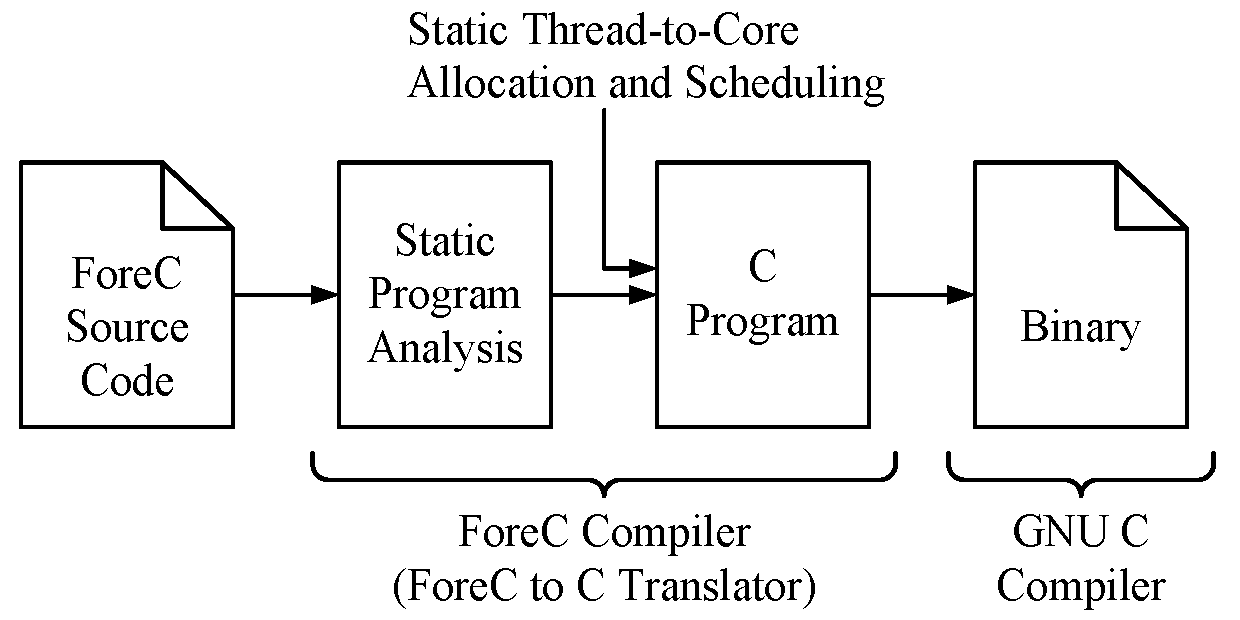
\includegraphics[width=0.6\columnwidth]{images/compilation_embedded_overview.pdf}

	\caption{Overview of compiling ForeC programs.}
	\label{fig:forec_compiling:overview}
\end{figure}

\begin{figure}
	\centering

	\begin{minipage}{0.47\columnwidth}
		\subfloat[Example ForeC program.]{
			\lstinputlisting[style=full]{./code/forec_compiling/example.forec}
			\label{fig:forec_compiling:example:forec}	
		}
	\end{minipage}
	\hspace{1cm}
	\begin{minipage}{0.25\columnwidth}
		\centering
		\subfloat[Total order.]{
			
\includegraphics[width=0.6\columnwidth]{total_order}
			\label{fig:forec_compiling:total_order}	
		}
		\vspace{1cm}
		\subfloat[Thread allocation.]{
			\begin{tabular}{c c c}
				{\bf Core 1}	&	& {\bf Core 2}	\\
				\cline{1-1}\cline{3-3}
				main			&	& tB			\\
				tA				&	& tD			\\
				tC				&	&				\\
			\end{tabular}
			\label{fig:forec_compiling:schedule}	
		}
	\end{minipage}
	
	\vfill
	
	\subfloat[Possible execution trace of the compiled program.]{
			
\includegraphics[width=0.65\columnwidth]{forec_timing}
			\label{fig:forec_compiling:timing}	
	}
	\caption{Example ForeC program to be compiled.}
\end{figure}


\subsection{Static Thread Scheduling}
\label{sec:forec_compiling:scheduling}
This section deals exclusively with ForeC threads.
We illustrate the static thread scheduling with the 
example of Figure~\ref{fig:forec_compiling:example:forec}. 
The programmer statically allocates the
threads to the cores and passes the allocations into the
compiler. The scheduling is \emph{static} and \emph{non-preemptive}
(cooperative). Thus, threads execute without interruption
until they reach a \emph{context-switching point}: a \verb$par$ or
\verb$pause$ statement, or the end of their body. 
The semantics of shared variables (see Section~\ref{sec:forec:shared_variables}) 
ensures that threads execute their local ticks in isolation, e.g., 
independently of their siblings or their parent's siblings.
The compiler defines a total order for all the threads.
The total order is based on the depth-first traversal of the thread hierarchy.
Figure~\ref{fig:forec_compiling:total_order} depicts the thread
hierarchy of the ForeC program from Figure~\ref{fig:forec_compiling:example:forec},
where numbers indicate the total order. A lower number
means higher execution priority.
Figure~\ref{fig:forec_compiling:schedule} shows a possible
thread allocation chosen by the programmer for two cores, in their thread scheduling
order. When a thread reaches a \verb$par$ statement, its 
child threads are forked for execution on their allocated
cores. The core that executes the parent thread is
called the \emph{master} core.
The cores that execute the child threads are called 
the \emph{slave} cores. Depending 
on the thread allocations, a core could be the master core 
of one thread and be the slave core of another 
thread. For the \verb$par$ statement on 
line~\ref{code:forec_compiling:forec_par1} of 
Figure~\ref{fig:forec_compiling:example:forec},
core 1 is the master core and core 2 is the slave core.

Based on the the thread allocation and scheduling order shown in 
Figure~\ref{fig:forec_compiling:schedule}, 
Figure~\ref{fig:forec_compiling:timing} is a possible execution trace.
The trace for both cores (``Core~1'' and ``Core~2'') 
progresses downwards from the top of Figure~\ref{fig:forec_compiling:timing}.
Thread executions are shown as white segments in the 
trace and each one has the thread's name and the executed 
lines of code from Figure~\ref{fig:forec_compiling:example:forec}.
The compiler generates \emph{synchronization routines} to 
manage the thread executions on the master and slave
cores. These routines are shown as shaded segments in the 
trace and each one has the routine's name. 
The names are prefixed with ``\verb$m$'' or ``\verb$s$'' 
to identify whether a routine is for a master or slave 
core, respectively. The names are suffixed with an integer 
to identify the unique id assigned to each \texttt{par} (with a 
depth-first traversal of the thread hierarchy starting from the root).
For example, the \verb$mFork1$, 
\verb$sFork1$, \verb$mJoin1$, and \verb$sJoin1$ routines in 
Figure~\ref{fig:forec_compiling:timing} all
manage the threads forked by thread \verb$main$. 
Table~\ref{table:forec_compiling:routines}
summarizes the behavior of the routines. The 
\verb$mFork$ and \verb$sFork$ routines manage
the forking of child threads (Section~\ref{sec:forec_compiling:par}). The 
\verb$mJoin$ and \verb$sJoin$ routines manage
the joining of child threads (Section~\ref{sec:forec_compiling:par}). 
The \verb$mSync$ and \verb$sSync$ routines manage
the global tick synchronization of all the cores (Section~\ref{sec:forec_compiling:sync}).
In Figure~\ref{fig:forec_compiling:timing}, the synchronization 
between the routines are shown as arrows marked 
with the information that is sent. The information is an 
integer value that encodes the following execution states 
of a thread: 0 (\verb$TERM$) for thread termination, 1 and 
greater for the unique id of the \texttt{par} statement that 
is executing, and -1 
(\verb$OTHER$) for executing a \verb$pause$ statement
or for not executing a \verb$par$ statement.

\begin{table}
	\def\arraystretch{1.3}
	\tbl{Summary of the synchronization routines.\label{table:forec_compiling:routines}}{
		\begin{tabular}{| p{\columnwidth} |}
			\hline
			\texttt{mFork}:	Uses a non-blocking send to notify the slave 
							cores whether or not the parent thread has forked.		\\ 
			\texttt{sFork}:	Blocks until it receives whether or not the parent 
							thread has forked.										\\ \hline
			\texttt{mJoin}:	Blocks until it receives whether the child threads 
							on other cores have terminated. Then, it notifies 
							the slave cores whether the parent thread has resumed.	\\ 
			\texttt{sJoin}:	Uses a non-blocking send to notify the master core 
							whether or not its child threads have terminated. Then, 
							it blocks until it receives whether the parent thread 
							has resumed.											\\ \hline
			\texttt{mSync}:	Synchronizes with all the cores, performs the
							housekeeping tasks, and then synchronizes with all the 
							cores again to start the next global tick.				\\ 
			\texttt{sSync}:	Synchronizes with all the cores and waits for the 
							next synchronization to start the next global tick.		\\ \hline
			\texttt{mAbort} and \texttt{sAbort}:	Evaluates the preemption 
							condition of an \texttt{abort}.							\\
			\hline
		\end{tabular}
	}
\end{table}

\begin{figure}
	\centering

	\begin{minipage}{0.4\columnwidth}
%		\subfloat[node.h]{
			\lstinputlisting[style=full]{./code/forec_compiling/linkednode.c}
%			\label{fig:forec_compiling:linkednode}
%		}
	\end{minipage}
%	\hspace{1cm}
%	\begin{minipage}{0.3\columnwidth}
%		\subfloat[insert(n1,n2)]{
%			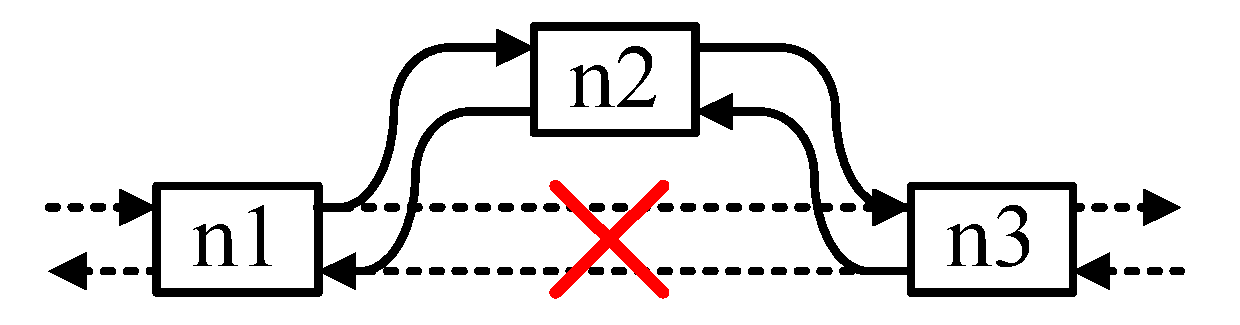
\includegraphics[width=\columnwidth]{images/list_insert.pdf}
%			\label{fig:forec_compiling:list_insert}	
%		}
%		\vspace{1cm}
%		\subfloat[remove(n2)]{
%			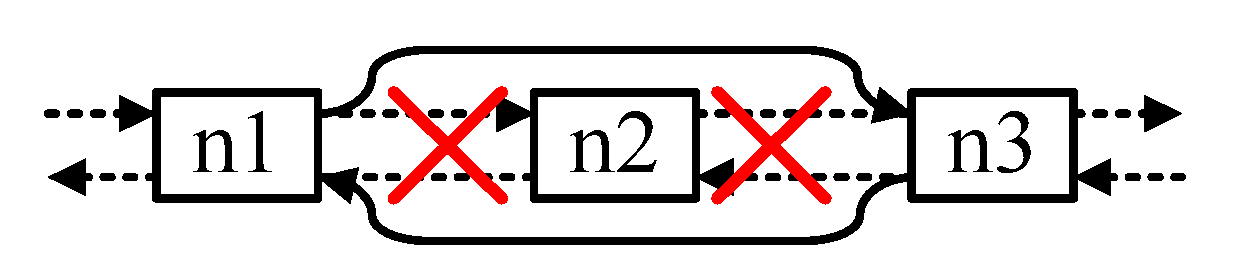
\includegraphics[width=\columnwidth]{images/list_remove.pdf}
%			\label{fig:forec_compiling:list_remove}	
%		}
%	\end{minipage}

	\caption{Definition of a linked list node and its operations in \texttt{node.h}.}
	\label{fig:forec_compiling:linkednode}
\end{figure}

The threads and synchronization routines are statically 
scheduled on each core with \emph{doubly linked lists}. 
Each node (defined in Figure~\ref{fig:forec_compiling:linkednode}) 
of a linked list represents a thread or a synchronization
routine and stores its continuation point (\verb$pc$) and
the links to its adjacent nodes (\verb$prev$ and
\verb$next$). A node's \verb$pc$ is initially set to the
start of the thread or routine's body. Each core starts its
scheduling by jumping to the \verb$pc$ of its first node.
When a context-switching point is reached during the
execution of a thread or routine, a jump is made to the
\verb$pc$ of the next node. A core will only execute the
threads and routines in its linked list. Thus, inserting or
removing a thread or routine from the list controls whether
it is included or excluded, respectively, from execution. 
The remainder of this section describes how a ForeC program is
compiled into a C program and how the linked lists are created
and used to implement the ForeC semantics. 


\subsection{Structure of the Generated Program}
Figure~\ref{fig:forec_compiling:example:c1} 
shows a simplified version of the C program generated for the
ForeC program in Figure~\ref{fig:forec_compiling:example:forec}. 
All line numbers in section refer to Figure~\ref{fig:forec_compiling:example:c1}.
The generated C program contains:
\begin{itemize} 
	\item The global declarations and functions from the ForeC program
		  (lines~\ref{code:forec_compiling:example_user1}--\ref{code:forec_compiling:example_user2}).
	\item The global declarations for storing the execution states of the threads and implementing the shared variables 
		  (lines~\ref{code:forec_compiling:example_scheduling1}--\ref{code:forec_compiling:example_copies}).
	\item The \verb$main$ function (line~\ref{code:forec_compiling:example_forecmain})
		  with the bootup routine (lines~\ref{code:forec_compiling:example_scheduler1}--\ref{code:forec_compiling:example_direct2}),
		  the synchronization routines 
		  (lines~\ref{code:forec_compiling:example_mFork1}--\ref{code:forec_compiling:example_scheduler2}), 
		  and the threads (lines~\ref{code:forec_compiling:example_threads1}--\ref{code:forec_compiling:example_threads2}). 
\end{itemize}
Although the scheduling routines dominate the generated code 
in Figure~\ref{fig:forec_compiling:example:c1}, their code remains constant 
whatever the size of the user-defined threads (which could be arbitrarily large).
When the cores enter the \verb$main$ function, they execute
the bootup routine to initialize their linked lists. First, 
a node is created for each thread and each synchronization routine
(lines~\ref{code:forec_compiling:example_scheduling3}--\ref{code:forec_compiling:example_scheduling4}). 
Second, the nodes are linked together to create the initial
linked list for each core (lines~\ref{code:forec_compiling:example_direct1}--\ref{code:forec_compiling:example_direct2}).
These initial lists are illustrated in the second row of 
Table~\ref{tab:forec_compiling:lists}. The threads and 
routines are inlined into the \verb$main$ function because fast
context-switching is implemented by jumping between C labels
with GNU's computed \verb$goto$ extension. Jumping with \verb$goto$ 
is restricted to C labels located in the same function scope. To avoid the need to 
create stacks for each thread to maintain their local variables, 
the local variables are given unique names and hoisted up to the 
global scope (e.g., \verb$tC$'s local variable
\verb$a$ on line~\ref{code:forec_compiling:example_a}). 
However, functions executed on the same core will
share the same stack space. To avoid stack corruption, all the
functions must execute atomically, i.e., without interruption. 

\begin{figure}
	\centering

	\lstinputlisting[style=fulltight,multicols=2,frame=tlr,lastline=120]{./code/forec_compiling/example.c}

	\caption{Example of the C program generated for Figure~\ref{fig:forec_compiling:example:forec}.}
	\label{fig:forec_compiling:example:c1}
\end{figure}

\begin{figure}
	\ContinuedFloat 
	\centering

	\lstinputlisting[style=fulltight,multicols=2,frame=lrb,firstline=121,firstnumber=121]{./code/forec_compiling/example.c}

	\caption{(Continued.) Example of the C program generated for Figure~\ref{fig:forec_compiling:example:forec}.}
	\label{fig:forec_compiling:example:c2}
\end{figure}


\subsection{The \texttt{par} Statement}
\label{sec:forec_compiling:par}
The execution of a ForeC program starts with its \verb$main$
thread. The slave cores must wait for their allocated
threads to be forked. \emph{The global tick in which threads fork and
join can only be determined at runtime.} Hence, before a core
executes a thread, it must check that no other higher
priority thread allocated to it will be forked. Otherwise,
the higher priority thread must be executed first. This is
achieved by scheduling an \verb$mFork$ routine after a
parent thread completes its local tick. It uses a
\emph{non-blocking send} to notify the slave cores whether
or not the parent thread has forked. Thus, a slave core uses
an \verb$sFork$ routine to \emph{block} until it receives
whether or not the parent thread has forked. To ensure
correct scheduling order, the \verb$sFork$ routine has the
same execution priority as the parent thread. When a fork
does occur, the \verb$mFork$ and \verb$sFork$ routines
instruct their cores to suspend the parent thread and to
schedule the child thread. In the first 
global tick of Figure~\ref{fig:forec_compiling:timing},
\verb$mFork1$ notifies \verb$sFork1$ that thread \verb$main$
has not forked (\verb$OTHER$ is sent). In the second global tick, 
\verb$mFork1$ notifies \verb$sFork1$ that thread \verb$main$
has forked (\verb$1$ is sent).

Before a core executes a parent thread that was suspended by
a fork, it must check that all of its child threads have
terminated. This is achieved by scheduling an \verb$mJoin$
routine after the child threads on the master core have
completed their respective local ticks. It \emph{blocks}
until it receives whether or not the child threads on the
slave cores have terminated. When all child threads have
terminated, the \verb$mJoin$ routine instructs the master
core to resume the parent thread. Thus, each slave core
schedules an \verb$sJoin$ routine after its child threads
complete their respective local ticks. It uses a
\emph{non-blocking send} to notify the master core whether
or not the child threads on the slave core have terminated. 
In the second and third global ticks of 
Figure~\ref{fig:forec_compiling:timing}, \verb$sJoin1$
notifies \verb$mJoin1$ that thread \verb$tB$ has 
terminated (\verb$TERM$ is sent).

\begin{table}
	\centering
	\tbl{Core 1 and 2's initial lists and subsequent lists when threads fork.\label{tab:forec_compiling:lists}}{
		\begin{tabular}{| c | l |}
			\hline
			\textbf{Execution Point}		& \multicolumn{1}{c|}{\textbf{Linked Lists}}														\\
			\hline
			When the program starts			& \raisebox{0.15cm}{\textbf{Core 1:}} 
\includegraphics[height=0.55cm]{images/list_m1.pdf}			\\
											& \raisebox{0.15cm}{\textbf{Core 2:}} 
\includegraphics[height=0.55cm]{images/list_s1.pdf}			\\ \hline
			When \texttt{main} \par forks (id = 1)	& \raisebox{0.15cm}{\textbf{Core 1:}} 
\includegraphics[height=0.50cm]{images/list_m2.pdf}	\\
											& \raisebox{0.15cm}{\textbf{Core 2:}} 
\includegraphics[height=0.49cm]{images/list_s2.pdf}			\\ \hline
			When \texttt{tB} \par forks (id = 2)	& \raisebox{0.15cm}{\textbf{Core 1:}} 
\includegraphics[height=0.49cm]{images/list_m3.pdf}	\\
											& \raisebox{0.15cm}{\textbf{Core 2:}} 
\includegraphics[height=0.50cm]{images/list_s3.pdf}			\\
			\hline
		\end{tabular}
	}
\end{table}

We now describe the C code that is generated for each
\verb$par$ statement and how the synchronization routines
are incorporated into the linked lists. 
The last two rows of Table~\ref{tab:forec_compiling:lists} 
visualizes core 1 and~2's linked 
lists when threads \verb$main$ and \verb$tB$ fork 
(lines~\ref{code:forec_compiling:example_par1} and 
\ref{code:forec_compiling:example_par2} respectively). 
Each \verb$par$ 
statement is assigned a unique positive integer 
\verb$id$ by the compiler.
Lines~\ref{code:forec_compiling:example_par1}--\ref{code:forec_compiling:example_join1}
in Figure~\ref{fig:forec_compiling:example:c1} is an 
example of the C code that is generated for a \verb$par$ 
statement. Line~\ref{code:forec_compiling:example_state}
sets the parent thread's execution state to \verb$id$
and sets the 
parent thread's \verb$pc$ to be immediately after the 
\verb$par$ statement. Line~\ref{code:forec_compiling:example_switch}
is a context-switch to the parent thread's 
\verb$mFork$ routine. 
Lines~\ref{code:forec_compiling:example_mFork1}--\ref{code:forec_compiling:example_mFork1_end}
is an example of the C code that is generated for an 
\verb$mFork$ routine. Line~\ref{code:forec_compiling:example_send1}
sends the parent thread's execute state to the slave cores.
If the parent thread has forked, then 
lines~\ref{code:forec_compiling:example_mAbort1_insert}--\ref{code:forec_compiling:example_mFork1_goto1}
insert the allocated child threads and an \verb$mJoin$ 
routine into the linked list. The parent thread and 
\verb$mFork$ routine are removed from the linked list.
If a child thread can fork its own threads,
then further \verb$mFork$ and \verb$sFork$ routines need to be
inserted into the linked lists. This ensures that the nested
threads can be forked. 
The end of line~\ref{code:forec_compiling:example_mFork1_goto1} is
a context-switch to the first node that was inserted. 
Otherwise, if the parent thread has not forked, then
line~\ref{code:forec_compiling:example_mFork1_goto2} is
a context-switch to the next node in sequence.

Recall that the slave cores have an \verb$sFork$
routine in their initial linked list. 
Lines~\ref{code:forec_compiling:example_sFork1}--\ref{code:forec_compiling:example_sFork1_end}
is an example of the C code that is generated for an \verb$sFork$
routine. Line~\ref{code:forec_compiling:example_receive1}
blocks until it receives whether the parent thread has
forked. If the parent thread has forked, then 
line~\ref{code:forec_compiling:example_sAbort1_insert}
inserts the allocated child threads and an \verb$sJoin$
routine into the linked list. The \verb$sFork$ routine 
is removed from the linked list. The end of 
line~\ref{code:forec_compiling:example_sFork1_goto1} is
a context-switch to the first node that was inserted.
Otherwise, if the parent thread has not forked, then
line~\ref{code:forec_compiling:example_sFork1_goto2} is
a context-switch to the next node in sequence.

Lines~\ref{code:forec_compiling:example_term1}--\ref{code:forec_compiling:example_term4} 
in Figure~\ref{fig:forec_compiling:example:c1} is an example 
of the C code that is generated for the end of a child 
thread to handle thread termination. 
Line~\ref{code:forec_compiling:example_term2} sets the thread's
execution state to \verb$TERM$. 
Line~\ref{code:forec_compiling:example_term3} removes the thread
from the linked list. 
Line~\ref{code:forec_compiling:example_term4} is a context-switch 
to the next node in sequence.
Lines~\ref{code:forec_compiling:example_mJoin1}--\ref{code:forec_compiling:example_mJoin1_end} 
is an example of the C code that is generated for an 
\verb$mJoin$ routine. 
Line~\ref{code:forec_compiling:example_receive2} blocks 
until it receives the execution state of each child thread.
If all the child threads have terminated, then 
line~\ref{code:forec_compiling:example_receive2_term1}
sets the execution state of the parent thread to \verb$OTHER$
and sends that state to the slave cores. 
Lines~\ref{code:forec_compiling:example_receive2_term2}--\ref{code:forec_compiling:example_receive2_term3}
insert the parent thread back into the linked list and 
removes the nodes associated with the \verb$par$ statement. 
This is followed by a context-switch to the parent thread.
Otherwise, if some child threads have not terminated, then
line~\ref{code:forec_compiling:example_receive2_term4} is 
is a context-switch to the next node in sequence.
Lines~\ref{code:forec_compiling:example_sJoin1}--\ref{code:forec_compiling:example_sJoin1_end}
is an example of the C code that is generated for an 
\verb$sJoin$ routine. 
Line~\ref{code:forec_compiling:example_send2} sends the 
execution state of each child thread to the master core.
Line~\ref{code:forec_compiling:example_sJoin1_receive}
blocks until it receives whether the parent thread has
been resumed. If the parent thread has been resumed, then
line~\ref{code:forec_compiling:example_sJoin1_term} removes
the \verb$sJoin$ routine from the linked list. 
Line~\ref{code:forec_compiling:example_sJoin1_goto} is a 
context-switch to the next node in sequence.


\subsection{The \texttt{pause} Statement}
The \verb$pause$ statement is a context-switching point and 
lines~\ref{code:forec_compiling:example_pause1}--\ref{code:forec_compiling:example_pause1_end} 
in Figure~\ref{fig:forec_compiling:example:c1}
is an example of the C code that is generated.
Line~\ref{code:forec_compiling:example_pause2} sets the
current thread's \verb$pc$ to be immediately after
the \verb$pause$ statement.
Line~\ref{code:forec_compiling:example_pause3} is a 
context-switch to the next node in sequence.
In the next global tick, execution will resume from statement 
immediately after the \verb$pause$ statement.


\subsection{Shared Variables}
Shared variables are hoisted up to the program's global 
scope to allow all cores to access them (e.g., 
line~\ref{code:forec_compiling:example_user1} in 
Figure~\ref{fig:forec_compiling:example:c1}). The copies of 
shared variables are implemented as unique global variables 
(e.g., line~\ref{code:forec_compiling:example_copies}) to
allow them to be combined on different cores. In each 
thread, all shared variable 
accesses are replaced by accesses to their copies
(e.g., lines~\ref{code:forec_compiling:example_x_main} and 
\ref{code:forec_compiling:example_x_tA}). 
The shared variables are copied at the start of each 
local tick, i.e., start of each 
thread body, and after each \verb$pause$ 
and \verb$par$ statement. For example, the shared variable
\verb$x$ on line~\ref{code:forec_compiling:example_user1}
is copied by thread \verb$main$ on 
lines~\ref{code:forec_compiling:example_copy1}, 
\ref{code:forec_compiling:example_copy2} and 
\ref{code:forec_compiling:example_copy3}.
As defined by the (\ref{forec:par-4}), (\ref{forec:par-5}), 
(\ref{forec:par-6}), and (\ref{forec:par-7}) semantic rules 
given in Section~\ref{sec:forec_semantics:sos}, 
the \verb$par$ statement is responsible for combining the copies
of shared variables. More precisely, when the child threads
of a \verb$par$ statement complete their respective local ticks,
their copies of shared variables are combined. The combined
result is assigned to their parent thread. This combine process
is implemented by the \verb$mJoin$ routine (e.g., 
line~\ref{code:forec_compiling:example_combine2}) because it 
waits for the child threads to complete their respective local 
ticks. The final values of the shared variables are computed 
by the \verb$mJoin$ routine of thread \verb$main$.


\subsection{The \texttt{abort} Statement}
We begin by describing the C code that is generated 
for an \verb$abort$ that does not have the optional 
\verb$immediate$ or \verb$weak$ keywords. 
Conditional jumps, using the preemption condition, 
are inserted after each \verb$pause$ statement in the 
\verb$abort$ body. For example, 
lines~\ref{code:forec_compiling:example_abort1}--\ref{code:forec_compiling:example_abort3} 
in Figure~\ref{fig:forec_compiling:example:c1} is an 
\verb$abort$ and a conditional jump is inserted on 
line~\ref{code:forec_compiling:example_abort2} 
after the \verb$pause$ statement.
The preemption condition \verb$x>1$ is used 
in the conditional jump. If the preemption 
condition evaluates to \emph{true}, a jump is
made to the statement immediately after the
\verb$abort$ (e.g., line~\ref{code:forec_compiling:example_abort4}).
If a \verb$par$ statement is inside
the \verb$abort$ body, then the preemption condition must be
evaluated before the threads can execute. For example, 
in the third global tick of Figure~\ref{fig:forec_compiling:timing},
the cores use the \verb$mAbort$ and \verb$sAbort$ routines to evaluate
the preemption condition on 
line~\ref{code:forec_compiling:forec_preemption} of 
Figure~\ref{fig:forec_compiling:example:forec}. It is safe to 
evaluate the preemption conditions in parallel because 
they are side-effect free by definition (Section~\ref{sec:forec:preemption}).
Thus, when a fork occurs, an \verb$Abort$ routine 
is inserted before the child threads in the linked lists. 
For a master core, 
lines~\ref{code:forec_compiling:example_mAbort1}--\ref{code:forec_compiling:example_mAbort1_end} 
in Figure~\ref{fig:forec_compiling:example:c1} 
is an example of the C code that is generated for an 
\verb$mAbort$ routine. 
Line~\ref{code:forec_compiling:example_mAbort1_1} 
evaluates the preemption condition. If it evaluates
to \emph{true}, then line~\ref{code:forec_compiling:example_mAbort1_2}
removes the nodes associated with the \verb$par$ statement.
Line~\ref{code:forec_compiling:example_mAbort1_3} sets the 
parent thread's \verb$pc$ to be immediately after the
\verb$abort$ statement and context-switches to the parent
thread. Otherwise, if the preemption condition evaluates
to \emph{false}, then line~\ref{code:forec_compiling:example_mAbort1_4}
is a context-switch to the next node in sequence.
For a slave core, 
lines~\ref{code:forec_compiling:example_sAbort1}--\ref{code:forec_compiling:example_sAbort1_end} 
is an example of the C code that is generated for an \verb$sAbort$
routine and is similar to that of an \verb$mAbort$.
Line~\ref{code:forec_compiling:example_sAbort1_1}
evaluates the preemption condition. If it evaluates
to \emph{true}, then line~\ref{code:forec_compiling:example_sAbort1_2}
removes the nodes associated with the \verb$par$ statement.
Line~\ref{code:forec_compiling:example_sAbort1_3} is a 
context-switch to the next node in sequence. Otherwise, 
if the preemption condition evaluates
to \emph{false}, then line~\ref{code:forec_compiling:example_sAbort1_4}
is a context-switch to the next node in sequence.

\begin{figure}
	\centering

	\begin{minipage}{0.28\columnwidth}
		\vspace{0.67cm}
		\subfloat[Immediate and strong \texttt{abort}.]{
			\lstinputlisting[style=fulltight,numbers=none]{./code/forec_compiling/immediate_abort.c}
			\label{fig:forec_compiling:immediate_abort}	
		}
	\end{minipage}
	\hfill
	\begin{minipage}{0.25\columnwidth}
		\vspace{0.67cm}
		\subfloat[Non-immediate and weak \texttt{abort}.]{
			\lstinputlisting[style=fulltight,numbers=none]{./code/forec_compiling/weak_abort.c}
			\label{fig:forec_compiling:weak_abort}	
		}
	\end{minipage}
	\hfill
	\begin{minipage}{0.31\columnwidth}
		\subfloat[Immediate and weak \texttt{abort}.]{
			\lstinputlisting[style=fulltight,numbers=none]{./code/forec_compiling/immediate_weak_abort.c}
			\label{fig:forec_compiling:immediate_weak_abort}	
		}
	\end{minipage}

	\caption{C code for the immediate and weak variants of the \texttt{abort} on 
			lines~\ref{code:forec_compiling:example_abort1}--\ref{code:forec_compiling:example_abort3} 
			of Figure~\ref{fig:forec_compiling:example:c1}.}
\end{figure}

The optional \verb$immediate$ keyword allows the preemption
condition to be evaluated before the \verb$abort$ body is
executed for the first time. Thus, an additional conditional 
jump, using the preemption condition, is inserted at the 
start of the \verb$abort$ body. Figure~\ref{fig:forec_compiling:immediate_abort}
is an example of the C code that would be generated if the \verb$abort$ on 
lines~\ref{code:forec_compiling:example_abort1}--\ref{code:forec_compiling:example_abort3} 
in Figure~\ref{fig:forec_compiling:example:c1} was 
an immediate \verb$abort$.
The optional \verb$weak$ keyword delays the jumping to the 
end of the \verb$abort$ body when the preemption condition
evaluates to \emph{true}. Thus, the conditional jump is separated
into two parts: (1) the evaluation of the preemption condition
and (2) the resulting jump. The evaluation is inserted directly 
after each \verb$pause$ statement and the jump is inserted 
directly before each \verb$pause$ statement. If a \verb$par$ 
statement is inside the weak \verb$abort$, then the 
\verb$mAbort$ and \verb$sAbort$ routines are inserted after 
the child threads in the linked lists. 
Figure~\ref{fig:forec_compiling:weak_abort}
is an example of the C code that would be generated if the \verb$abort$ on 
lines~\ref{code:forec_compiling:example_abort1}--\ref{code:forec_compiling:example_abort3} 
in Figure~\ref{fig:forec_compiling:example:c1} was 
a weak \verb$abort$. 
Figure~\ref{fig:forec_compiling:immediate_weak_abort} 
is an example of the C code generated if it was an 
immediate and weak \verb$abort$.


\subsection{Global Tick Synchronization}
\label{sec:forec_compiling:sync} 
The notion of a global tick is preserved by ending each linked 
list with a \verb$Sync$ routine that implements \emph{barrier synchronization}. 
This synchronization is shown at the end of each global tick in 
Figure~\ref{fig:forec_compiling:timing}.
For the master core that executes the \verb$main$ thread, 
lines~\ref{code:forec_compiling:example_mSync}--\ref{code:forec_compiling:example_mSync_end} 
is an example of the C code that is generated for 
an \verb$mSync$ routine.
Line~\ref{code:forec_compiling:example_mSync_1} is a 
barrier synchronization for the end of the tick. 
Line~\ref{code:forec_compiling:example_mSync_2} 
performs the following housekeeping tasks: finalizing the
values of the shared variables, emitting outputs, and
sampling inputs.
Line~\ref{code:forec_compiling:example_mSync_3} is 
a barrier synchronization to signal the start of the 
next global tick. 
Line~\ref{code:forec_compiling:example_mSync_4} is a
context-switch to the first node in the linked list.
For the remaining slave cores, 
lines~\ref{code:forec_compiling:example_sSync}--\ref{code:forec_compiling:example_scheduler2}
is an example of the C code that is generated for an
\verb$sSync$ routine.
Line~\ref{code:forec_compiling:example_sSync_1} are
barrier synchronizations for the end of the tick
and the start of the next tick. This is followed by 
a context-switch to the first node in the linked list.

%\subsection{Optimizations}
%Inlined nesting of \verb$par$ statements (each nested 
%\verb$par$ statement is not in sequence with any other 
%statement): Fork and join all the nested threads together.
%
%Shared variable that does not need a combine function: Assign
%the writer's copy directly to the shared variable.
%
%Shared variable that is only read by a thread: Apart from the
%thread's first local tick (where the parent's copy is read), 
%the shared variable can be read in subsequent local ticks.


\subsection{Generating Programs for Execution on Operating Systems}
\label{sec:forec_compiling:posix}
This section describes how the ForeC compiler is extended to
generate executable code for operating systems. 
To utilize multiple cores in a system, a program
must create multiple threads that the operating system can 
schedule. We modify the ForeC compiler to generate a 
Pthread~\cite{multiprocessor_pthreads} for each core in the system. Each
Pthread is responsible for executing the ForeC threads
statically allocated to the same core, as shown in
Figure~\ref{fig:forec_compiling:os}. In effect, a fixed pool of
Pthreads executes the ForeC threads and the cost of creating
each Pthread is only incurred once. Although the
Pthreads will be dynamically scheduled by the operating
system, the original ForeC threads will still follow their
static schedule. Finally, the generated 
Pthreads program is compiled with a GNU C compiler.

\begin{figure}
	\centering

	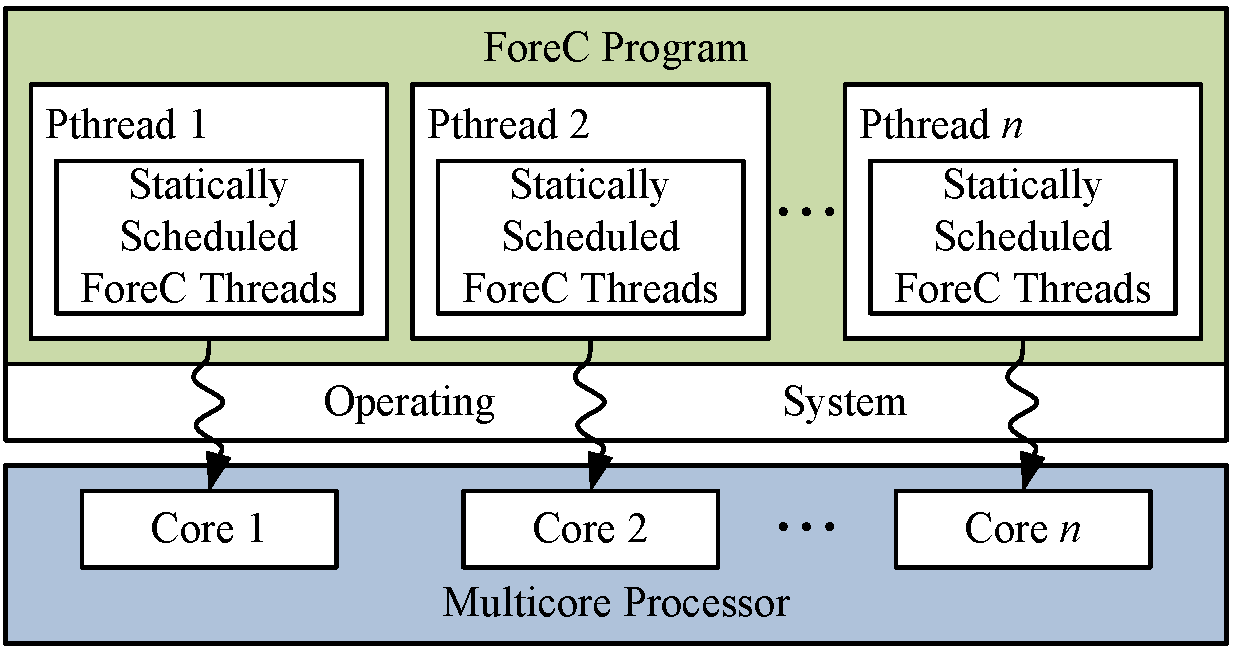
\includegraphics[width=0.7\columnwidth]{images/compilation_os.pdf}

	\caption{Using Pthreads to adapt the generated code for multi-cores.}
	\label{fig:forec_compiling:os}
\end{figure}

\begin{figure}
	\centering

	\begin{minipage}{0.85\columnwidth}
		\lstinputlisting[style=fulltight]{./code/forec_compiling/example_desktop.c}
	\end{minipage}

	\caption{Example Pthreads program.}
	\label{fig:forec_compiling:example:c:desktop}
\end{figure}

For the ForeC program of Figure~\ref{fig:forec_compiling:example:forec}, 
Figure~\ref{fig:forec_compiling:example:c:desktop} is a 
simplified extract of the generated Pthreads program. 
In addition to the global declarations shown in 
Figure~\ref{fig:forec_compiling:example:c1}, there are
now Pthreads-related declarations
(lines~\ref{code:forec_compiling:example:desktop:pthread1}--\ref{code:forec_compiling:example:desktop:pthread2}) 
and a new \verb$main$ function for creating the 
Pthreads~(line~\ref{code:forec_compiling:example:desktop:main}).
The original \verb$main$ function from Figure~\ref{fig:forec_compiling:example:c1} 
(line~\ref{code:forec_compiling:example_forecmain}) 
is renamed as \verb$forecMain$ (line~\ref{code:forec_compiling:example:desktop:forecmain}).
When the operating system executes the \verb$main$
function, the Pthreads start executing the 
\verb$forecMain$ function and, hence, the statically 
allocated ForeC threads.


\subsection{Discussion}
This section has presented the compilation of ForeC
programs for direct execution on parallel hardware architectures. 
The compilation is syntax-driven and templates are
used to generate code for each ForeC construct. Light-weight
synchronization routines are generated to manage the forking
and joining of threads across the cores. The use of linked
lists to manage the scheduling of threads and routines is
inspired by that of the Columbia Esterel Compiler~\cite{timed_cec}.
The code generation
is structural, meaning that a nesting of ForeC constructs is
compiled into a nesting of each construct's generated code.
The advantages with our static scheduling approach include: 
(1) a light-weight scheduling of ForeC threads, and
(2) analysis is easier because all scheduling decisions are 
known beforehand.
However, the disadvantages include:
(1) the inability to dynamically load balance the ForeC threads 
to utilize the idle cores, and
(2) the need to recompile the program to target a different 
number of cores.
Memory fences in C (e.g.,
\texttt{atomic\_thread\_fence}~\cite{programming_languages_c11}) 
are not used to implement the semantics of shared
variables because (1) the reading of inputs and the writing
of outputs for global tick synchronisation already requires
barrier synchronization among the cores, making memory fences 
redundant for the finalizing shared variables, and (2) memory fences
on shared variables are unable to isolate the accesses of
one thread from the accesses of another thread, which is needed
during each local tick.


For future work, the dynamic scheduling of 
ForeC threads can be developed to improve the average-case 
performance on desktop computers. 
In future versions of the compiler, we also wish to implement 
proper thread stacks to allow the execution of functions 
that pause.

The distribution of traditional synchronous programs over multiple 
processors is not new~\cite{distributed_reactive_systems_survey,distributed_synchronous_dependency_driven,distributed_reactive_systems_automatic,wcrt_esterel_multicores,YuanYR11,timed_esterel_distribution_emperor,timed_multiclock_multithreaded}.
It is motivated by the desire to execute computations closer
to their inputs and outputs, which may be distributed over a
geographical area. Unfortunately, the use of signals for
instantaneous communication makes compilation notoriously
difficult. First, \emph{causality analysis}~\cite{timed_compiling_esterel} 
is needed to ensure that the presence or absence of all signals
can be determined exactly in each global tick. Second, the compiler 
must generate code for resolving signal statuses at runtime.
A common approach is to compile away the parallelism and to generate
a sequential program~\cite{timed_cec,timed_compiling_esterel}.
Third, the sequential program is partitioned into subprograms 
and distributed to execute on their allocated processors. 
Desynchronization techniques~\cite{BenvenisteCG00,GiraultNP06,distributed_synchronous_desynchronize_modes} 
can be used when the processors execute and communicate at different speeds. 
SynDEx~\cite{distributed_synchronous_semantics_preserving} is 
a tool that automatically distributes synchronous programs and 
considers the cost of communication between the processors.
In contrast, ForeC is significantly easier to compile because thread
communication is delayed with shared variables 
(Section~\ref{sec:forec:shared_variables}). Causality analysis
is not required and ForeC threads can be distributed directly
to the available cores. The parallelism specified by
the programmer is preserved by the ForeC compiler and a
sequential intermediate code is not required.

With the advent of multi-cores, the distribution of
synchronous programs is motivated by the desire to improve
their execution performance. The distribution of synchronous
programs over multi-threaded and multi-core reactive processors
has been studied extensively~\cite{LiH12,YuanAYRS09,DayaratneRS06,SalcicHRB06,timed_esterel_distribution_emperor}. 
Reactive processors handle the scheduling of threads
in hardware, thereby simplifying the code generation. However, 
causality analysis is still required and signal statuses 
still need to be resolved at runtime. Signal resolution may 
reduce a program's parallel performance because a thread 
must wait for a signal's status to be resolved before it 
can be read. There have been studies on the parallelization 
of synchronous programs on general-purpose 
multi-cores~\cite{wcrt_esterel_multicores,YuanYR11,multiprocessing_openmp_synchronous}.
These approaches extract a parallel program from a 
sequential representation of the original synchronous program. 
Due to control and signal dependencies, the opportunities 
for extracting parallelism from a sequential program is
limited. In contrast, execution dependencies only exist
at the local tick boundaries of ForeC threads (recall that each
thread operates on a local copy of each shared variable). As a result, ForeC 
threads have more opportunity to execute in parallel.


%\begin{itemize}
%	\item PTARM related compilation for enforcing a constant global tick length 
%		  which removes the need synchronize the hardware threads 
%		  using busy waiting.
%		  Replace the first barrier() with a "delay until" the wcrt expires.
%		  Replace the second barrier() with a "delay until" the housekeeping task completes.
%\end{itemize}


%\section{Benchmarking}
\section{ForeC Benchmarking}
\label{sec:forec_benchmarking}
This section quantitatively assesses ForeC's parallel
execution performance on a mixture of data and control
dominated benchmark programs. ForeC's execution performance
is compared with that of Esterel, a widely used synchronous
language for concurrent safety-critical systems that has 
inspired some features of ForeC, and that of
OpenMP, a popular desktop solution for parallel programming.
The static timing analysis of ForeC using the reachability
technique is described in a previous paper~\cite{YipRAG13}. 
The benchmark results~\cite{YipRAG13} showed that the worst-case
reaction time~\cite{wcrt_concurrent_reactive} (WCRT) of 
ForeC programs could be estimated to a high degree of precision,
which is very useful for implementing real-time embedded systems in
general, and time-predictable systems in particular. 
We highlight some of the key findings in this section.


\subsection{Benchmark Programs}
This section describes the benchmark programs used in
the evaluations:
\begin{itemize}
	\item \texttt{FlyByWire} is based on the real-time UAV benchmark 
		  called PapaBench~\cite{benchmark_papabench}. \verb$FlyByWire$
		  is a control dominated program with several tasks 
		  managing the UAV's motors, navigation, timer, and 
		  operation mode.
		  
	\item \texttt{FmRadio} \cite{streaming_openmp_extension} is 
		  based on the GNU Radio Package~\cite{benchmark_gnu_radio}, which 
		  transforms a fixed stream of radio signals into 
		  audio. The history of the radio signals 
		  is used to determine how the remaining stream of 
		  signals should be transformed. \verb$FmRadio$ is data orientated.
		  
	\item \texttt{Life} simulates Conway's Game of Life~\cite{Gardner70} for a fixed
		  number of iterations and a given grid of cells. In each iteration
		  of the simulation, the outcome of each cell can be computed 
		  independently. \verb$Life$ has a good 
		  mixture of data and control dominated computations.
		  
	\item \texttt{Lzss} uses the Lempel-Ziv-Storer-Szymanski (LZSS~\cite{benchmark_lzss}) 
		  algorithm to compress a fixed amount of text. Multiple
		  sliding windows are used to search different parts of the 
		  text for repeated segments that can compressed. \verb$Lzss$ has
		  a good mixture of data and control dominated computations.
		  
	\item \texttt{Mandelbrot} computes the Mandelbrot
		  set for a square region of the complex number plane. The
		  Mandelbrot set for each point in the region can be computed 
		  independently, making \verb$Mandelbrot$ a data-parallel program.
		  
	\item \texttt{MatrixMultiply} computes the matrix
		  multiplication of two equally sized square matrices. Each
		  element in the resulting matrix can be computed independently,
		  making \verb$MatrixMultiply$ a data-parallel program.
\end{itemize}


\subsection{Performance Evaluation}
\label{sec:forec_benchmarking:performance}
The performance of ForeC is evaluated against that of Esterel,
a traditional synchronous language, and OpenMP,
a general-purpose parallel programming extension to C. 
We create C (non-multi-threaded), ForeC, 
Esterel, and OpenMP versions of each benchmark program 
and handcrafted each for best performance. 
We use \emph{Speedup} as the performance metric to compare ForeC, 
Esterel, and OpenMP:
\begin{equation*}
	Speedup(P) = \frac{\text{Execution time of the C sequential version}}{\text{Execution time of }P}
\end{equation*}
where $P$ is either the ForeC, Esterel, or OpenMP version of 
the benchmark program being tested.
Hence, the speedups of ForeC, Esterel, and OpenMP are always
with respect to the execution time of the C version.
The higher the speedup the better.


\subsubsection{Comparison with Esterel}
The approaches by Yuan et al.~\cite{YuanYR11,Yuan13} for
parallelizing the execution of Esterel programs has been shown
to perform well on an Intel multi-core and on a
(simulated) Xilinx MicroBlaze multi-core. However, only
compiler support is available for Yuan et al.'s
dynamic scheduling approach on MicroBlaze multi-core. Thus,
we evaluate ForeC against Esterel on a MicroBlaze
multi-core and use the dynamic scheduling approach to
parallelize the Esterel programs. The static scheduling
approach presented in Section~\ref{sec:forec_compiling} is used
to parallelize the ForeC programs. 
Yuan et al.'s dynamic scheduling approach uses a special hardware 
FIFO queue to allocate the threads to the cores. Each core retrieves 
a thread from the queue and executes it until it terminates or 
reaches a context-switching point for resolving signal statuses. 
A core makes a context-switch by adding the executing thread back 
to the queue and retrieving a different thread from the queue. 
Threads are added to the queue when they are forked by other threads. 
Threads are removed from the queue when they terminate. All the cores 
can access the FIFO queue in parallel and each access takes two clock 
cycles to complete. For benchmarking, the MicroBlaze 
multi-core simulator described in 
Section~\ref{sec:introduction:pret:multicore} is extended 
with a hardware queue to support the dynamic scheduling. 
The configuration of the simulator is shown in 
Figure~\ref{fig:results_embedded_specs}. 

\begin{figure}
	\centering
	\def\arraystretch{1.3}
	\begin{tabular}{|p{\textwidth}|}
		\hline
		Xilinx MicroBlaze, 4 physical cores, three-stage pipeline, no speculative	
		features (no branch prediction,	caches, or out-of-order execution), 
		16 KB private data and instruction scratchpads on each core (1 cycle access time), 
		64 KB global memory (5 cycle access time), TDMA shared bus (5 cycle time slots per			
		core), Benchmarks compiled with GCC-4.1.2 -O0.
		\\ \hline
	\end{tabular}
	
	\caption{MicroBlaze multi-core configuration.}
	\label{fig:results_embedded_specs}
\end{figure}

\begin{table}
	\centering
	\def\arraystretch{1.3}
	\tbl{ForeC versus Esterel benchmarks.\label{tab:results_embedded_prog}}{
		\begin{tabular}{l c c l c c}
			\hline
									& \multicolumn{2}{c}{\bf Lines of Code}		& & \multicolumn{2}{c}{\bf Number of Threads}	\\ \cline{2-3}\cline{5-6}
			{\bf Benchmark}			& {\bf ForeC}	& {\bf Esterel}				& & {\bf ForeC}	& {\bf Esterel}					\\
			\hline
			\texttt{Life}			& 212			& 139+111					& & 4 (4)		& 7 (4)							\\ 
			\texttt{Lzss}			& 485			& 42+421					& & 4 (4)		& 4 (4)							\\ 
			\texttt{Mandelbrot}		& 381			& 220+337					& & 8 (8)		& 18 (9)						\\ 
			\texttt{MatrixMultiply}	& 162			& 51+53						& & 16 (8)		& 16 (8)						\\ 
			\hline
		\end{tabular}
	}
\end{table}

Table~\ref{tab:results_embedded_prog} shows the
implementation details of the ForeC and Esterel versions of
the benchmark programs. Esterel is suited for specifying
control concurrency, but is not so for specifying
data dominated computations. Esterel allows data 
computations to be delegated to external host functions,
defined in a host language such as C. Hence, for the ``Lines
of Code'' column in Table~\ref{tab:results_embedded_prog},
the first number is the lines of Esterel code and the second
number is the lines of host C-code (excluding header files).
The ``Number of Threads'' column specifies the total number of
threads forked by the programs and, in brackets, the total
number of threads that can execute together in parallel. The
benchmark programs are compiled for bare-metal execution
and do not need operating system support. Yuan et al.'s
compilation approach~\cite{Yuan13} uses an intermediate
format called GRaph Code (GRC)~\cite{timed_compiling_esterel}, which
transforms the program into an acyclic execution graph. The
GRC helps schedule the resolution of signals, executing 
the GRC from the top to the bottom corresponds to one tick
of the program. To decide which GRC states need to be executed during
each tick, a set of internal variables are updated as
the GRC is executed. Compared to GRC, for most programs, the 
ForeC compiler (see Section~\ref{sec:forec_compiling})
can generate more efficient code that require less context-switching.
The same input vector is given to the ForeC and
Esterel versions of a benchmark program to ensure
that the same computations are performed. When a program
terminates, the simulator returns the execution
time in clock cycles.

Figure~\ref{fig:results_embedded} shows the speedups
achieved by ForeC and Esterel when the benchmark programs
execute on four cores. Apart from \verb$MatrixMultiply$,
ForeC shows superior performance compared to Esterel, even
though Esterel uses dynamic scheduling with hardware
acceleration. The need to resolve instantaneous signal
communication in Esterel can lead to significant runtime
overheads. All possible signal emitters must execute before
any signal consumers can execute and this invariant is 
achieved using a signal locking protocol~\cite{Yuan13} that 
is costly. In comparison, shared
variables in ForeC only need to be resolved at the end of
each tick. The significance of the overhead is
evident in the \verb$Mandelbrot$ results, where the Esterel version
has 24 unique signals and only achieves a speedup of
1.2$\times$ on four cores. In fact, when \verb$Mandelbrot$ is
executed on one core, Esterel's execution time is already 58\%
longer than the C version. ForeC's execution time is only
0.2\% longer than the C version. For \verb$MatrixMultiply$, the
fork-join pattern was used by ForeC and Esterel. Because of
minimal data dependencies in \verb$MatrixMultiply$, combine functions
are not needed in the ForeC version and signals
are not needed in the Esterel version. Thus, the scheduling
overheads for the ForeC and Esterel versions are minimal,
resulting in very similar speedup values. 

\begin{figure}
	\centering

	\begin{tikzpicture}
		\begin{axis}[
			ybar = 0,
			footnotesize,
			width = 10.1cm, height = 6cm,
		%
			ylabel = Average Speedup Normalized to Baseline (Sequential),
			ylabel style = {align = center, text width = 6cm},
			ymax = 4, ymin = 0,
			ytick = {\pgfkeysvalueof{/pgfplots/ymin}, ..., \pgfkeysvalueof{/pgfplots/ymax}},
			ymajorgrids = true,
		%
			xtick = data,
			symbolic x coords = {Life, Lzss, Mandelbrot, MatrixMultiply},
			xtick pos = left,
			enlarge x limits = {abs = 1cm},
		%
			legend columns = -1,
			legend style = {at = {(0.5, 1.05)}, anchor = south},
			legend image code/.code = {\draw[#1] (0cm, -0.12cm) rectangle (0.6cm, 0.15cm);}  
		]
			\addplot[blue, pattern = horizontal lines, pattern color = blue] table[x = program, y = speedup, row sep = \\] {
				program			speedup	\\
				Life			1		\\ 
				Lzss			1		\\
				Mandelbrot		1 		\\
				MatrixMultiply	1 		\\
			};

			\addplot[red, pattern = north east lines, pattern color = red] table[x = program, y = speedup, row sep = \\] {
				program			speedup	\\
				Life			2.28	\\
				Lzss			2.42	\\
				Mandelbrot		1.20	\\
				MatrixMultiply	3.87	\\
			};

			\addplot[black!30!green, pattern = dots, pattern color = black!30!green] table[x = program, y = speedup, row sep = \\] {
				program			speedup	\\
				Life			3.25	\\ 
				Lzss			3.30	\\
				Mandelbrot		3.68 	\\
				MatrixMultiply	3.76 	\\
			};

			\legend{Baseline (Sequential C), Esterel, ForeC}
		\end{axis}
	\end{tikzpicture}

	\caption{Average speedup results for ForeC and Esterel on four cores normalized to sequential runtime. 
			 Platform details in Figure~\ref{fig:results_embedded_specs}.}
	\label{fig:results_embedded}	
\end{figure}

\begin{figure}
	\centering
	\def\arraystretch{1.3}
	\begin{tabular}{|p{\textwidth}|}
		\hline
		Intel Core-i5 3570 at 3.4 Ghz, 4 physical cores,
		Hyper-Threading disabled, Turbo Boost disabled,
		SpeedStep disabled, 3 MB L3 data-cache,
		Linux 3.6, 8 GB of RAM, Benchmarks compiled with GCC-4.8 -O2.
		\\ \hline
	\end{tabular}
	
	\caption{Intel multi-core configuration.}
	\label{fig:results_desktop_specs}
\end{figure}

\subsubsection{Comparison with OpenMP}
Table~\ref{tab:results_desktop_prog} shows the
implementation details of the ForeC and OpenMP versions of
the benchmark programs. Intel VTune Amplifier XE 2013~\cite{vtune} 
software was used during the development and testing of the
parallelized benchmarks. The software is useful in
providing insight into the regions of code which are the
most time consuming and therefore top candidates for
parallelization. It is also used to calculate the total
runtimes and to show the number of cores being used 
during the execution of each benchmark.
Figure~\ref{fig:results_desktop_specs} shows the
specifications of the desktop computer on which all testing
is carried out.

\begin{table}
	\centering
	\def\arraystretch{1.3}
	\tbl{ForeC versus OpenMP benchmarks.\label{tab:results_desktop_prog}}{
		\begin{tabular}{l c c l c}
			\hline
									& \multicolumn{2}{c}{\bf Lines of Code}	&	& {\bf Number of Threads}	\\ \cline{2-3}\cline{5-5}
			{\bf Benchmark}			& {\bf ForeC}	& {\bf OpenMP}			&	& {\bf ForeC}				\\
			\hline
			\texttt{FlyByWire}		& 241			& 227					&	& 8 (7)						\\ 
			\texttt{FmRadio}		& 481			& 382					&	& 12 (6)					\\ 
			\texttt{Life}			& 325 			& 268					&	& 10 (8) 					\\ 
			\texttt{Lzss}			& 593 			& 552					&	& 4 (4) 					\\ 
			\texttt{Mandelbrot}		& 111 			& 89					&	& 4 (4)						\\ 
			\texttt{MatrixMultiply}	& 156			& 121					&	& 7 (4)						\\ 
			\hline
		\end{tabular}
	}	
\end{table}

\begin{figure}
	\centering

	\begin{tikzpicture}
		\begin{axis}[
			ybar = 0,
			footnotesize,
			width = \columnwidth, height = 6cm,
		%
			ylabel = Average Speedup Normalized to Baseline (Sequential),
			ylabel style = {align = center, text width = 6cm},
			ymax = 4, ymin = 0,
			ytick = {\pgfkeysvalueof{/pgfplots/ymin}, ..., \pgfkeysvalueof{/pgfplots/ymax}},
			ymajorgrids = true,
		%
			xtick = data,
			symbolic x coords = {FlyByWire, FmRadio, Life, Lzss, Mandelbrot, MatrixMultiply},
			xtick pos = left,
			enlarge x limits = {abs = 1cm},
		%
			legend columns = -1,
			legend style = {at = {(0.5, 1.05)}, anchor = south},
			legend image code/.code = {\draw[#1] (0cm, -0.12cm) rectangle (0.6cm, 0.15cm);}  
		]
			\addplot[blue, pattern = horizontal lines, pattern color = blue] table[x = program, y = speedup, row sep = \\] {
				program			speedup	\\
				FlyByWire		1		\\
				FmRadio			1		\\
				Life			1 		\\
				Lzss			1		\\
				Mandelbrot		1 		\\
				MatrixMultiply	1 		\\
			};

			\addplot[red, pattern = north east lines, pattern color = red] table[x = program, y = speedup, row sep = \\] {
				program			speedup	\\
				FlyByWire		3.80	\\
				FmRadio			2.02	\\
				Life			2.82 	\\
				Lzss			3.46 	\\
				Mandelbrot		2.04 	\\
				MatrixMultiply	3.35	\\
			};

			\addplot[black!30!green, pattern = dots, pattern color = black!30!green] table[x = program, y = speedup, row sep = \\] {
				program			speedup	\\
				FlyByWire		2.42	\\
				FmRadio			2.63	\\
				Life			2.98 	\\
				Lzss			3.90	\\	
				Mandelbrot		3.88 	\\
				MatrixMultiply	3.90 	\\
			};

			\legend{Baseline (Sequential C), OpenMP, ForeC}
		\end{axis}
	\end{tikzpicture}

	\caption{Average speedup results for ForeC and OpenMP on four cores normalized to sequential runtime. 
			 Platform details in Figure~\ref{fig:results_desktop_specs}.}
	\label{fig:results_desktop}	
\end{figure}

Figure~\ref{fig:results_desktop} shows the speedups achieved by ForeC
and OpenMP when the benchmark programs are executed over four
cores. The speedups are averaged over 200 executions of each program to
take into account the potential effects of long term use, e.g., filling
and flushing of the cache, and background kernel processes on the computer. ForeC
and OpenMP are able to achieve a speedup factor of between two and
four over four cores. However, from the results it is clear that in most
cases ForeC produces a greater speedup factor, barring two
exceptions. Firstly, OpenMP is more suited and delivered a much higher
speedup factor in \verb$FlyByWire$. Secondly, for \verb$Mandelbrot$,
the OpenMP version is unable to utilize all four available cores.

We would like to mention that we used dynamic and static thread
scheduling pragmas in OpenMP. Static scheduling is used in benchmarks
(e.g., \verb$FlyByWire$) when we could determine at compile time the so 
called \emph{chunk size} (the amount of work and number of loop iterations 
that each thread needs to perform). Dynamic scheduling is used in benchmarks 
(e.g., \verb$MatrixMultiply$ and \verb$Mandelbrot$) when the chunk size of 
each thread could not be made equal or could not be determined at compile 
time. For dynamic scheduling, the chunk size of each thread is determined
by the OpenMP runtime. Using dynamic scheduling does introduce slight overheads,
especially thread locking, but these overheads should be amortized over
the overall run of the benchmarks. This OpenMP scheduling approach is in
stark contrast to the ForeC approach, where all work scheduling is
static and determined automatically by the ForeC compiler, whereas in
OpenMP all work scheduling is the programmer's burden.


\subsection{Time Predictability}
We developed a C++ static timing analysis
tool~\cite{YipRAG13}, called ForeCast, that statically
analyzes the WCRT of ForeC programs on embedded multi-core
processors. We highlight the key findings of our previous
paper~\cite{YipRAG13} on the static WCRT analysis of ForeC
programs executed on embedded multi-cores.
Benchmarking is performed on the MicroBlaze multi-core
simulator with the configuration shown in
Figure~\ref{fig:results_embedded_static_specs} and
ForeCast itself is executed on a 2.20 GHz Intel Core 2 Duo
computer with 3 GB RAM and Linux 2.6.38. We
highlight the results of the benchmark program
called \verb$802.11a$~\cite{streaming_openmp_extension}.
\verb$802.11a$ is production code from Nokia that tests
various signal processing algorithms needed to decode
802.11a data transmissions. \verb$802.11a$ has both complex
data and control dominated computations. \verb$802.11a$ has 
2147 lines of ForeC code and forks up to 26 threads, of which 
10 can execute in parallel. \verb$802.11a$ is 
distributed on up to 10 cores and ForeCast is used to 
compute the WCRT of each possible distribution. 
The WCRT computed by ForeCast is taken as the \emph{computed} WCRT.
To evaluate the tightness of the computed WCRTs, \verb$802.11a$ 
is executed on the MicroBlaze simulator for one million 
global ticks or until the program terminates. Test
vectors are generated to elicit the worst-case program state by
studying the program's control-flow. The simulator returns
the execution time of each global tick and the longest is
taken as the \emph{observed} WCRT. 

\begin{figure}
	\centering
	\def\arraystretch{1.3}
	\begin{tabular}{|p{\textwidth}|}
		\hline
		Xilinx MicroBlaze, three-stage pipeline, no speculative	
		features (no branch prediction,	caches, or out-of-order execution), 
		8 KB private data and instruction scratchpads on each core 
		(1 cycle access time), 32 KB global memory 
		(5 cycle access time), TDMA shared bus (5 cycle time slots per			
		core and, thus, a $5\times$(number of cores) 
		cycles long bus schedule), Benchmarks compiled with MB-GCC-4.1.2 -O0 and 
		decompiled with MB-OBJDUMP-4.1.2.
		\\ \hline
	\end{tabular}
	
	\caption{MicroBlaze multi-core configuration.}
	\label{fig:results_embedded_static_specs}
\end{figure}

\begin{figure}
	\centering

	\begin{minipage}[t]{6.5cm}
		\begin{tikzpicture}
			\begin{axis}[
				footnotesize,
				width = 6.5cm, height = 6cm,
				grid = major,
			%
				tick scale binop=\times,
				ylabel = WCRT (clock cycles),
				ymax = 200000, ymin = 0,
				ytick = {0, 25000, 50000, 75000, 100000, 125000, 150000, 175000, 200000},
				scaled y ticks = base 10:-3,
			%
				xlabel = Cores,
				xtick = data,
				xmax = 10, xmin = 1,
				xtick = {\pgfkeysvalueof{/pgfplots/xmin}, ..., \pgfkeysvalueof{/pgfplots/xmax}},
			%
				legend columns = -1,
				legend style = {at = {(0.5, 1.15)}, anchor = south},
			]
				\addplot[red, mark = triangle] table[x = core, y = time, row sep = \\] {
					core	time	\\
					1		152297	\\
					2		94518	\\
					3		70453	\\
					4		60858	\\
					5		53573	\\
					6		56308	\\
					7		64783	\\
					8		72998	\\
					9		75238	\\
					10		83248	\\
				};

				\addplot[blue, mark = o] table[x = core, y = time, row sep = \\] {
					core	time	\\
					1		154306	\\
					2		95545	\\
					3		71390	\\
					4		61765	\\
					5		53930	\\
					6		57605	\\
					7		66470	\\
					8		75005	\\
					9		77630	\\
					10		84505	\\
				};
			
				\legend{Observed, Computed}
			\end{axis}
		\end{tikzpicture}
		\caption{WCRT results for \texttt{802.11a} in clock cycles.}
		\label{fig:forec_benchmarking:benchmark_wcrt}
	\end{minipage}
	\hfill
	\begin{minipage}[t]{6.5cm}
		\begin{tikzpicture}
			\begin{axis}[
				footnotesize,
				width = 6.5cm, height = 6cm,
				grid = major,
			%
				ylabel = Over-estimation (\%),
				ymax = 3.5, ymin = 0,
				ytick = {0, 0.5, 1, 1.5, 2, 2.5, 3, 3.5},
			%
				xlabel = Cores,
				xtick = data,
				xmax = 10, xmin = 1,
				xtick = {\pgfkeysvalueof{/pgfplots/xmin}, ..., \pgfkeysvalueof{/pgfplots/xmax}},
			]
				\addplot[red, mark = triangle] table[x = core, y = time, row sep = \\] {
					core	time	\\
					1		1.3		\\
					2		1.1		\\
					3		1.3		\\
					4		1.5		\\
					5		0.6		\\
					6		2.4		\\
					7		2.6		\\
					8		2.7		\\
					9		3.2		\\
					10		1.5		\\
				};
			\end{axis}
		\end{tikzpicture}
	
		\caption{WCRT over-estimations for \texttt{802.11a}.}
		\label{fig:forec_benchmarking:benchmark_wcrt_over}
	\end{minipage}
\end{figure}

The observed and computed WCRTs of \verb$802.11a$ (in clock
cycles) are plotted as a line graph in
Figure~\ref{fig:forec_benchmarking:benchmark_wcrt}. This
graph shows that the static timing analysis is very
precise, even when the number of cores increases. 
The \emph{over-estimation} of the computed WCRT 
can be calculated as follows:
\begin{equation*}
	\text{WCRT Over-estimation} = \frac{\text{Computed WCRT} - \text{Observed WCRT}}{\text{Observed WCRT}} \times 100\%
\end{equation*}
Figure~\ref{fig:forec_benchmarking:benchmark_wcrt_over} 
exemplifies the WCRT over-estimations for 
\verb$802.11a$ as a line graph. We can see that
ForeCast computes WCRTs that are at most 3.2\% longer than the
observed WCRTs. This shows that extremely time predictable 
systems can be designed with ForeC.

The computed WCRTs of \verb$802.11a$ 
in Figure~\ref{fig:forec_benchmarking:benchmark_wcrt} 
reflect the benefit of multi-core execution. The 
computed WCRT decreases when the number of cores 
is increased from one to five cores. The computed
WCRT at five cores corresponded to the
execution time of one thread which is already allocated to
its own core. Thus, the WCRT could not be improved by
distributing the remaining threads. The WCRT increases after
five cores because of the increasing scheduling overheads and
cost of accessing global memory. These costs reduce the
benefit of multi-core execution. 

\begin{figure}
	\subfloat[\texttt{Life}.] {
		\begin{tikzpicture}
			\begin{axis}[
				footnotesize,
				width = 6.5cm, height = 6cm,
				grid = major,
			%
				tick scale binop=\times,
				ylabel = WCET (clock cycles),
				ymax = 6000000, ymin = 0,
				ytick = {0, 1000000, 2000000, 3000000, 4000000, 5000000, 6000000},
				scaled y ticks = base 10:-6,
			%
				xlabel = Cores,
				xtick = data,
				xmax = 4, xmin = 1,
				xtick = {\pgfkeysvalueof{/pgfplots/xmin}, ..., \pgfkeysvalueof{/pgfplots/xmax}},
			%
				legend columns = -1,
				legend style = {at = {(0.5, 1.15)}, anchor = south},
			]
				\addplot[red, mark = triangle] table[x = core, y = time, row sep = \\] {
					core	time	\\
					1		5332852	\\
					2		2923933	\\
					3		2854608	\\
					4		1608143	\\
				};

				\addplot[blue, mark = o] table[x = core, y = time, row sep = \\] {
					core	time	\\
					1		3707623	\\
					2		1989424	\\
					3		2160169	\\
					4		1125504	\\
				};
				
				\legend{Esterel observed, ForeC observed}
			\end{axis}
		\end{tikzpicture}
	}
	\hfill
	\subfloat[\texttt{Lzss}.] {
		\begin{tikzpicture}
			\begin{axis}[
				footnotesize,
				width = 6.5cm, height = 6cm,
				grid = major,
			%
				tick scale binop=\times,
				ylabel = WCET (clock cycles),
				ymax = 60000000, ymin = 0,
				ytick = {0, 10000000, 20000000, 30000000, 40000000, 50000000, 60000000},
				scaled y ticks = base 10:-7,
			%
				xlabel = Cores,
				xtick = data,
				xmax = 4, xmin = 1,
				xtick = {\pgfkeysvalueof{/pgfplots/xmin}, ..., \pgfkeysvalueof{/pgfplots/xmax}},
			]
				\addplot[red, mark = triangle] table[x = core, y = time, row sep = \\] {
					core	time		\\
					1		49612714	\\
					2		30498189	\\
					3		29296659	\\
					4		18188259	\\
				};

				\addplot[blue, mark = o] table[x = core, y = time, row sep = \\] {
					core	time		\\
					1		44109533	\\
					2		23282661	\\
					3		23769071	\\
					4		13338631	\\
				};
			\end{axis}
		\end{tikzpicture}
	}

	\subfloat[\texttt{Mandelbrot}.] {
		\begin{tikzpicture}
			\begin{axis}[
				footnotesize,
				width = 6.5cm, height = 6cm,
				grid = major,
			%
				tick scale binop=\times,
				ylabel = WCET (clock cycles),
				ymax = 40000000, ymin = 0,
				ytick = {0, 5000000, 10000000, 15000000, 20000000, 25000000, 30000000, 35000000, 40000000},
				scaled y ticks = base 10:-7,
			%
				xlabel = Cores,
				xtick = data,
				xmax = 4, xmin = 1,
				xtick = {\pgfkeysvalueof{/pgfplots/xmin}, ..., \pgfkeysvalueof{/pgfplots/xmax}},
			]
				\addplot[red, mark = triangle] table[x = core, y = time, row sep = \\] {
					core	time		\\
					1		37827004	\\
					2		26236151	\\
					3		21169386	\\
					4		19912651	\\
				};

				\addplot[blue, mark = o] table[x = core, y = time, row sep = \\] {
					core	time		\\
					1		23943425	\\
					2		12375556	\\
					3		9409536		\\
					4		6501186		\\
				};
			\end{axis}
		\end{tikzpicture}
	}
	\hfill
	\subfloat[\texttt{MatrixMultiply}.] {
		\begin{tikzpicture}
			\begin{axis}[
				footnotesize,
				width = 6.5cm, height = 6cm,
				grid = major,
			%
				tick scale binop=\times,
				ylabel = WCET (clock cycles),
				ymax = 60000000, ymin = 0,
				ytick = {0, 10000000, 20000000, 30000000, 40000000, 50000000, 60000000},
				scaled y ticks = base 10:-7,
			%
				xlabel = Cores,
				xtick = data,
				xmax = 4, xmin = 1,
				xtick = {\pgfkeysvalueof{/pgfplots/xmin}, ..., \pgfkeysvalueof{/pgfplots/xmax}},
			]
				\addplot[red, mark = triangle] table[x = core, y = time, row sep = \\] {
					core	time		\\
					1		50404272	\\
					2		26022038	\\
					3		26248728	\\
					4		13027758	\\
				};

				\addplot[blue, mark = o] table[x = core, y = time, row sep = \\] {
					core	time		\\
					1		50934944	\\
					2		26280962	\\
					3		26647997	\\
					4		13417662	\\
				};
			\end{axis}
		\end{tikzpicture}
	}

	\caption{Observed WCETs for ForeC and Esterel. Platform details in Figure~~\ref{fig:results_embedded_specs}.}
	\label{fig:forec_benchmarking:benchmark_wcrt_forec_esterel}
\end{figure}

We perform additional experiments to compare the 
observed worst-case execution times (WCETs) of ForeC and 
Esterel versions of \texttt{Life}, \texttt{Lzss}, \texttt{Mandelbrot},
and \texttt{MatrixMultiply} on embedded
multi-cores. For our experiments, the WCET of a program
is the total time that it takes for the entire program to 
execute from start to finish.\footnote{The entire execution 
of a benchmark program occurs over multiple ticks.} We limit the 
\texttt{Life} program to simulate 10,000 iterations of the game.
The same input vector is given to the ForeC and Esterel versions 
of a benchmark program to ensure that the same computations are performed. 
The Esterel programs are compiled using Yuan
et al.'s approach~\cite{Yuan13}. For each benchmark program in 
Figure~\ref{fig:forec_benchmarking:benchmark_wcrt_forec_esterel}, 
the WCETs for ForeC and 
Esterel are plotted. Apart from \texttt{MatrixMultiply}, the
observed WCETs for ForeC are much shorter than those for Esterel. 
Unfortunately, the static timing
analysis of such multi-core Esterel programs has not been developed, 
preventing an objective comparison of time-predictability. To 
compute WCRTs for Esterel that are as tight as ForeCast, 
the dynamic resolution of signal statuses will need to be analyzed 
extremely carefully to rule out the infeasible runtime decisions.


\subsection{Discussion}
This section assessed the performance 
of ForeC on an embedded multi-core and desktop multi-core. 
The static timing analysis of ForeC programs was presented in
an earlier paper~\cite{YipRAG13}. In this section, 
on an embedded multi-core, most of the statically 
scheduled ForeC programs performed better than Yuan et al.'s~\cite{Yuan13} 
dynamically scheduled Esterel programs. This is because it is easier
to extract parallelism from ForeC programs, largely thanks to its
shared variable semantics (see Section~\ref{sec:forec:shared_variables}). 
Serializing Esterel
programs into GRC can obfuscate the parallelism and the need
to update internal state variables can add unnecessary
overhead. Runtime resolution is also needed to resolve
Esterel's instantaneous signal communication. Ju et
al.~\cite{wcrt_esterel_multicores} provide a multi-core 
static scheduling approach for Esterel. However, we cannot 
compare with that work because speedup results 
for multi-core execution were not reported. 

On a desktop
multi-core, ForeC's static scheduling approach proved to be
competitive against OpenMP, a dynamic runtime solution.
These are encouraging results for the use of ForeC to
develop high performing parallel programs. Moreover, determinism is
enforced by ForeC's formal semantics, not by a particular
runtime environment. There is much scope to improve the
ForeC compiler to generate more efficient code. For example, thread
allocations could be refined automatically by feeding the 
WCRT results of the ForeCast analyzer into the ForeC compiler until 
the WCRT cannot be reduced. 


%\section{Conclusions and Future Work}
\section{Conclusions and Future Directions}
\label{sec:conclusion}
A common approach to developing cyber-physical systems 
is to program an embedded ARM
multi-core with C and Pthreads and to use an RTOS
to manage the execution. Although high performance 
can be achieved with this approach, time predictability
is sacrificed. This paper proposed the ForeC language for 
the deterministic, parallel, and reactive 
programming of parallel architectures. Section~\ref{sec:forec}
provided an in-depth description of ForeC and, unlike existing 
C-based synchronous languages, it is designed specifically for 
parallel programming. The semantics of ForeC is designed to give 
programmers the ability to express many forms of parallel patterns
while ensuring that ForeC programs can be compiled efficiently
for parallel execution and be amenable to static timing 
analysis. ForeC's main innovation 
revolves around its shared variable semantics that provides 
thread isolation and deterministic communication. The behavior
of a shared variable can be tailored to the application at hand
by specifying a suitable \emph{combine function} and \emph{policy}. All 
ForeC programs are correct by construction (no race conditions,
no deadlocks) 
because mutual exclusion constructs are not needed. The formal 
semantics greatly simplifies the understanding and debugging
of parallel programs.
Section~\ref{sec:forec_compiling} presented a compilation approach
that used non-preemptive static thread scheduling. The key 
strategy was to preserve the ForeC threads and to use light-weight
context-switching and simple scheduling routines to preserve the
ForeC semantics.

For future work, the ForeC compiler could be improved to generate more efficient
code that remains amenable to static timing analysis. In
particular, different static scheduling strategies could be
explored for different parallel patterns. Currently, scheduling 
priorities are assigned to ForeC threads by traversing the thread
hierarchy in a depth-first manner. However, assigning 
scheduling priorities in a breadth-first manner could produce 
more efficient schedules in some cases. The allocation of 
ForeC threads could be refined automatically by feeding the 
WCRT results of the ForeCast analyzer into the ForeC compiler.


% Appendix
\appendix
\section{Shared Variables}
\setcounter{section}{1}
\label{sec:forec_combine}
This appendix describes how shared variables are passed by
value or by reference into functions, and how the combine policies and combine
functions work together to combine more than two copies of a
shared variable. We compare the behaviors of the combine
policies, \verb$all$, \verb$new$, and \verb$mod$, using an
illustrative example. We also provide additional examples of
combine functions for primitive C data types and for
programmer-specified data structures. 

\subsection{Passing Shared Variables by Value and by Reference}
\label{sec:forec_combine:passing}
Following the C convention, a function argument in ForeC can
be passed by value or by reference. An argument passed
by value can either be a shared or a private variable.
E.g., in Figure~\ref{fig:forec_combine:passing}, 
line~\ref{fig:forec_combine:passing_f_call} makes a
call to function \texttt{f} with the arguments \texttt{x} (a
shared variable) and \texttt{y} (a private variable).
Function \texttt{f} (line~\ref{fig:forec_combine:passing_f}) 
declares two variables \texttt{d} (a
private variable) and \texttt{e} (a shared variable) that
are initialized with the values $3$ (from \texttt{x}) and
$5$ (from \texttt{y}), respectively.

When passed by reference, the address
of the function's argument is copied into the function's parameter.
Changes made to the dereferenced parameter are made to
the argument. The syntax for a function parameter
that passes a shared variable by reference should begin with
``\texttt{shared}~\emph{data\_type}\texttt{*}~\emph{p}''. 
This follows the C convention for other type qualifiers such 
as ``\texttt{const}'', where ``\texttt{const~int*~p}''
declares a pointer \texttt{p} to a constant \texttt{int} variable.
E.g., in Figure~\ref{fig:forec_combine:passing} on 
line~\ref{fig:forec_combine:passing_g}, the parameter of
function \texttt{g} declares a pointer \texttt{p} to a shared 
\texttt{int} variable. On line~\ref{fig:forec_combine:passing_g_call}, 
the ``\texttt{\&}'' unary 
operator is used to pass the shared variable \texttt{x} by 
reference into \texttt{g}.

Just like ``\texttt{int~const*~p}'' declares a constant pointer 
\texttt{p} to an \texttt{int} variable, ``\texttt{int shared* p}''
declares a shared pointer \texttt{p} to an \texttt{int} variable. 
This means that the address stored in \texttt{p} is shared among 
multiple threads. The final possibility is ``\texttt{shared~int~shared*~p}'' 
which declares a shared pointer \texttt{p} to a shared \texttt{int} 
variable.

\begin{figure}
	\centering

	\begin{minipage}[b]{0.8\textwidth}
		\lstinputlisting[style=full]{./code/forec/combine/passing.c}
	\end{minipage}

	\caption{Example of passing a shared variable by value and by reference.}
	\label{fig:forec_combine:passing}
\end{figure}

\newpage


\subsection{Combining More Than Two Copies}
\label{sec:forec_combine:copies}
The ForeC program shown in
Figure~\ref{fig:forec_combine:multiple_forec} is used to
explain how multiple copies of a shared variable are
combined. The program's control-flow graph is shown in
Figure~\ref{fig:forec_combine:multiple_cfg}. The program has
a shared variable called \verb$s$ that uses the combine
function \verb$plus$. The initial value of \verb$s$ is $3$ 
for the program's first tick.
Figure~\ref{fig:forec:combine_copies} shows the copies of
\verb$s$ at the end of the first tick, organized by the
thread genealogy. Each node represents a thread and the 
current value of its local
copy, e.g., {\setlength{\fboxsep}{3pt}\fbox{main: 3}} means
that the \verb$main$ thread has a local copy 
of \texttt{s} with the value $3$.
Copies that were assigned a value during the tick have the
$\bullet$ symbol, e.g., 
{\setlength{\fboxsep}{3pt}\fbox{tA: 1$\bullet$}} means that 
thread \verb$tA$'s copy has been assigned the value $1$. 
Arrows are drawn from the 
child threads to their parents to show the thread genealogy.
Threads \texttt{tC} and \texttt{tD} create their copies
from \verb$tA$'s copy (see Section~\ref{sec:forec:shared_variables_copying}). 
Hence, the value of thread \verb$tC$'s 
copy is $1$. Threads \texttt{tE} and \texttt{tF} create
their copies from \texttt{tB}'s copy.

\begin{figure}
	\centering

	\subfloat[ForeC program.] {
		\begin{minipage}[b]{0.5\textwidth}
			\lstinputlisting[style=full]{./code/forec/combine/multiple.forec}
			\label{fig:forec_combine:multiple_forec}
		\end{minipage}
	}
	\hfill
	\subfloat[Control-flow graph.]{
		
\includegraphics[width=0.45\columnwidth]{images/multiple_cfg}
		\label{fig:forec_combine:multiple_cfg}	
	}
	\caption{Example ForeC program.}
\end{figure}

\begin{figure}
	\centering

	\subfloat[The copies of \texttt{s} when tick 1 ends.]{
		
\includegraphics[height=3cm]{images/combine}
		\label{fig:forec:combine_copies}	
	}
	\hfill
	\subfloat[Policy \texttt{all}.]{
		
\includegraphics[height=3cm]{images/combine_all}
		\label{fig:forec:combine_all}	
	}

	\subfloat[Policy \texttt{new}.]{
		
\includegraphics[height=3cm]{images/combine_new}
		\label{fig:forec:combine_new}	
	}
	\hspace{3.9cm}
	\subfloat[Policy \texttt{mod}.]{
		
\includegraphics[height=3cm]{images/combine_mod}
		\label{fig:forec:combine_mod}	
	}
	\hspace{0.8cm}

	\caption{Effects of the combine policies.}
\end{figure}

The formal semantics of ForeC 
(Section~\ref{sec:forec_semantics}) defines how more than two
copies of a shared variable are combined. The 
copies from sibling threads (i.e., threads forked by 
the same \verb$par$ statement) are combined 
and the resulting combined value is assigned to their parent
thread. Then, the copies of the parent and its sibling 
are combined together and assigned to their parent. 
This continues until the \verb$main$ thread is reached.
Figure~\ref{fig:forec:combine_all} illustrates this
for the combine policy \verb$all$, where all the copies 
are combined. The final combined value is $11$ and
it is assigned to shared variable \verb$s$ to 
complete the global tick.

The combine policy \verb$new$ ignores the copies that have 
the same
value as their shared variable, which is not changed during 
the tick. For the copies shown
in Figure~\ref{fig:forec:combine_copies}, thread \verb$main$, \texttt{tB},
and \verb$tE$'s copies of \verb$s$ would be ignored.
Figure~\ref{fig:forec:combine_new} illustrates how the
copies are combined for the combine policy \verb$new$. Note
that thread \verb$tF$'s copy is assigned directly to
\verb$tB$ because its sibling's copy is ignored. The final
combined value is $8$.

For the combine policy \verb$mod$, the copies that have not
been assigned a value during the tick are ignored. For the
copies shown in Figure~\ref{fig:forec:combine_copies},
thread \verb$main$, \texttt{tB}, \verb$tC$, and \verb$tE$'s copies of 
\verb$s$ would be ignored.
Figure~\ref{fig:forec:combine_mod} illustrates how the
copies are combined for the combine policy \verb$mod$. The
final combined value is $7$.

%When combining two copies with a non-associative or
%non-commutative function (e.g., subtraction or division),
%the order that the copies are passed into the combine
%function can affect the results. To ensure deterministic
%combine behavior, a static order is used. The textual order
%that the child threads appear in their \verb$par$ statement
%is the order that their copies are passed into the combine
%function.


\subsection{Combine Policies Illustrated}
\label{sec:forec_combine:policies}
This section illustrates the behavior of the combine
policies \verb$all$, \verb$new$, and \verb$mod$ over
several ticks by using the example of
Figure~\ref{fig:forec_combine:button}.
Figure~\ref{fig:forec_combine:button_task} shows a block
diagram of the ForeC program of
Figure~\ref{fig:forec_combine:button_forec}. The
program outputs the number of times \texttt{button1} and
\texttt{button2} are pressed in each tick of the
program. On line~\ref{code:forec_combine:button_par} in
Figure~\ref{fig:forec_combine:button_forec}, threads
\verb$t1$ and \verb$t2$ are forked to check which 
buttons have been pressed. The results are assigned to the
shared variable \verb$count$.
Line~\ref{code:forec_combine:button_par} also forks thread
\verb$t3$ to read the value of \verb$count$ and to output it to
\verb$display$. Hence, three copies of \verb$count$ will be
created in each tick. The copies of
\verb$count$ are combined with the function \verb$plus$
(line~\ref{code:forec_combine:button_plus}) with 
the combine policy \texttt{mod}.
Figure~\ref{table:forec_combine:button_inputs} provides
possible input values for five ticks of the program.
For example, only \texttt{button1} is pressed in tick~$2$. 
Figure~\ref{table:forec_combine:button_mod}
shows the value of the shared variable
\texttt{count} and the value of each thread's local copy of \texttt{count}. 
The copies that were assigned a value during the
tick have the~$\bullet$ symbol. For tick~$1$, \texttt{count}~$= 0$, 
its initial value. From tick~$2$ 
onwards, the value of \texttt{count} corresponds to the number of 
button presses in the previous tick, because only
threads~\texttt{t1} and~\texttt{t2}'s modified copies are
combined.

Figure~\ref{table:forec_combine:button_new} illustrates the 
behavior of the combine policy \texttt{new} over several
ticks. The values of threads~\texttt{t1}, 
\texttt{t2}, and \texttt{t3}'s local copies 
are ignored when they have the same value as \texttt{count}.
Figure~\ref{table:forec_combine:button_all} illustrates the 
behavior of the combine policy \texttt{all} over several
ticks. In this case, threads~\texttt{t1}, \texttt{t2},
and \texttt{t3}'s local copies are always used
to compute the value of \texttt{count}. 
The value of \texttt{count} corresponds to the running
total of button presses, i.e., in tick~$6$ a total of four
button presses have occurred in previous ticks.

\begin{figure}
	\centering

	\subfloat[Button counter.]{
		
\includegraphics[width=0.5\columnwidth]{images/button_task}
		\label{fig:forec_combine:button_task}	
	}

	\subfloat[ForeC program of the button counter.] {
		\begin{minipage}[b]{0.68\textwidth}
			\lstinputlisting[style=full]{./code/forec/combine/button.forec}
			\label{fig:forec_combine:button_forec}
		\end{minipage}
	}
	
	\caption{Example of counting the number of button inputs.}
	\label{fig:forec_combine:button}
\end{figure}

\begin{figure}
	\footnotesize

	\subfloat[Possible input values.] {
		\begin{tabular}{l c c c c c l}
											& \multicolumn{6}{c}{\textbf{Tick}}																\\ \cline{2-7}
											& \textbf{1}	& \textbf{2}	& \textbf{3}	& \textbf{4}	& \textbf{5}	& \textbf{6}	\\
			\hline
			\texttt{button1}				& 0				& 1				& 1				& 1				& 0				& $\dotsb$		\\
			\texttt{button2}				& 0				& 0				& 1				& 0				& 0				& $\dotsb$		\\
			\hline
																																			\\
																																			\\
		\end{tabular}
		\label{table:forec_combine:button_inputs}
	}
	\hfill
	\subfloat[Combine policy \texttt{mod}.] {
		\begin{tabular}{l c c c c c l}
									& \multicolumn{6}{c}{\textbf{Tick}}																\\ \cline{2-7}
			\textbf{\texttt{count}}	& \textbf{1}	& \textbf{2}	& \textbf{3}	& \textbf{4}	& \textbf{5}	& \textbf{6}	\\
			\hline
			\texttt{t1}'s copy		& 0$\bullet$	& 1$\bullet$	& 1$\bullet$	& 1$\bullet$	& 0$\bullet$	& $\dotsb$		\\
			\texttt{t2}'s copy		& 0$\bullet$	& 0$\bullet$	& 1$\bullet$	& 0$\bullet$	& 0$\bullet$	& $\dotsb$		\\
			\texttt{t3}'s copy		& 0~			& 0~			& 1~			& 2~			& 1~			& $\dotsb$		\\
			\hline
			\texttt{count}			& 0~			& 0~			& 1~			& 2~			& 1~			& 0				\\
			\hline
		\end{tabular}
		\label{table:forec_combine:button_mod}
	}
	
	\subfloat[Combine policy \texttt{new}.] {
		\begin{tabular}{l c c c c c l}
									& \multicolumn{6}{c}{\textbf{Tick}}																\\ \cline{2-7}
			\textbf{\texttt{count}}	& \textbf{1}	& \textbf{2}	& \textbf{3}	& \textbf{4}	& \textbf{5}	& \textbf{6}	\\
			\hline
			\texttt{t1}'s copy		& 0$\bullet$	& 1$\bullet$	& 1$\bullet$	& 1$\bullet$	& 0$\bullet$	& $\dotsb$		\\
			\texttt{t2}'s copy		& 0$\bullet$	& 0$\bullet$	& 1$\bullet$	& 0$\bullet$	& 0$\bullet$	& $\dotsb$		\\
			\texttt{t3}'s copy		& 0~			& 0~			& 1~			& 1~			& 0~			& $\dotsb$		\\
			\hline
			\texttt{count}			& 0~			& 0~			& 1~			& 1~			& 0~			& 0				\\
			\hline
		\end{tabular}
		\label{table:forec_combine:button_new}
	}
	\hfill
	\subfloat[Combine policy \texttt{all}.] {
		\begin{tabular}{l c c c c c l}
									& \multicolumn{6}{c}{\textbf{Tick}}																\\ \cline{2-7}
			\textbf{\texttt{count}}	& \textbf{1}	& \textbf{2}	& \textbf{3}	& \textbf{4}	& \textbf{5}	& \textbf{6}	\\
			\hline
			\texttt{t1}'s copy		& 0$\bullet$	& 1$\bullet$	& 1$\bullet$	& 1$\bullet$	& 0$\bullet$	& $\dotsb$		\\
			\texttt{t2}'s copy		& 0$\bullet$	& 0$\bullet$	& 1$\bullet$	& 0$\bullet$	& 0$\bullet$	& $\dotsb$		\\
			\texttt{t3}'s copy		& 0~			& 0~			& 1~			& 3~			& 4~			& $\dotsb$		\\
			\hline
			\texttt{count}			& 0~			& 0~			& 1~			& 3~			& 4~			& 4				\\
			\hline
		\end{tabular}
		\label{table:forec_combine:button_all}
	}

	\caption{The value of \texttt{count} under each combine policy.}
\end{figure}

\newpage


\subsection{Examples of Combine Functions}
\label{sec:forec_combine:functions}
The simplest combine functions are those based on the 
associative and commutative binary mathematical operators: 
\begin{itemize}
	\item Arithmetic addition (\texttt{+}) and multiplication (\texttt{*});
	\item Logical AND (\texttt{\&\&}) and OR (\texttt{||});
	\item Bitwise AND (\texttt{\&}) and OR (\texttt{|});
	\item Minimum and maximum using \texttt{if}--\texttt{else} statement.
\end{itemize}
The combine functions should be associative and commutative so 
as to make the \texttt{par} statement commutative and associative,
relying only on the nesting of binary \texttt{par} statements
to fork more than two child threads at the same time
(e.g., \texttt{par(par(t$_1$,t$_2$),t$_3$) = par(t$_1$,par(t$_2$,t$_3$))}). 
The programmer is free to write combine functions
based on non-commutative or non-associative binary operators
(e.g., \texttt{-}, \texttt{/}, or \texttt{\%}),
but this will violate the hypothesis of the theorem for determinism 
(Theorem~\ref{thm:deterministic}).

%\begin{figure}
%	\centering
%	
%	\subfloat[Minimum of two values.] {
%		\begin{minipage}[b]{0.44\textwidth}
%			\lstinputlisting[style=full]{./code/forec/combine/min.c}
%		\end{minipage}
%	}
%	\hfill
%	\subfloat[Maximum of two values.] {
%		\begin{minipage}[b]{0.44\textwidth}
%			\lstinputlisting[style=full]{./code/forec/combine/max.c}
%		\end{minipage}
%	}
%	
%	\subfloat[Addition of two values.] {
%		\begin{minipage}[b]{0.44\textwidth}
%			\lstinputlisting[style=full]{./code/forec/combine/add.c}
%		\end{minipage}
%	}
%	\hfill
%	\subfloat[Multiplication of two values.] {
%		\begin{minipage}[b]{0.44\textwidth}
%			\lstinputlisting[style=full]{./code/forec/combine/mul.c}
%		\end{minipage}
%	}
%
%	\subfloat[Bitwise AND of two values.] {
%		\begin{minipage}[b]{0.44\textwidth}
%			\lstinputlisting[style=full]{./code/forec/combine/band.c}
%		\end{minipage}
%	}
%	\hfill
%	\subfloat[Bitwise OR of two values.] {
%		\begin{minipage}[b]{0.44\textwidth}
%			\lstinputlisting[style=full]{./code/forec/combine/bor.c}
%		\end{minipage}
%	}
%
%	\subfloat[Logical AND of two values.] {
%		\begin{minipage}[b]{0.44\textwidth}
%			\lstinputlisting[style=full]{./code/forec/combine/land.c}
%		\end{minipage}
%	}
%	\hfill
%	\subfloat[Logical OR of two values.] {
%		\begin{minipage}[b]{0.44\textwidth}
%			\lstinputlisting[style=full]{./code/forec/combine/lor.c}
%		\end{minipage}
%	}
%
%	\caption{Examples of combine functions for primitive C data types.}
%	\label{fig:forec_combine:primative}
%\end{figure}

Combine functions can also be defined for 
user-defined data structures. For example,
Figure~\ref{fig:forec_combine:prodsum} defines a C-struct
called \verb$ProdSum$ that stores the product (\verb$prod$)
and sum (\verb$sum$) of the numbers assigned to it. The
combine function \verb$prodsum$ multiplies all the values in
\verb$prod$ and sums all the values in \verb$sum$. An
example of its behavior is provided after the function as
comments. 

For another example, line~\ref{code:mins:struct} of
Figure~\ref{fig:forec_combine:mins} defines a C-struct
called \texttt{Min} that stores an assigned value
(\verb$value$) and tracks the minimum value that has
been assigned (\verb$min$). The combine function
(line~\ref{code:mins:combine}) reads the 
\texttt{value}s and assigns the minimum 
value to \texttt{res.min}. The minimum value is also 
assigned to \texttt{res.value},
so that it will be read when it is combined with another copy.
An example of its behavior is provided after the function as
comments. Indeed, the combine function will only behave in
an associative and commutative manner if the threads only
write to \verb$value$ and do not read from it.

%Combine functions can use the \texttt{orig} 
%of a shared variable to perform computations that relate to 
%past values.

\begin{figure}
	\centering

	\subfloat[Product and sum of two values.] {
		\begin{minipage}[b]{0.9\textwidth}
			\lstinputlisting[style=full]{./code/forec/combine/prodsum.c}
			\label{fig:forec_combine:prodsum}
		\end{minipage}
	}
	
	\subfloat[Minimum of two values.] {
		\begin{minipage}[b]{0.9\textwidth}
			\lstinputlisting[style=full]{./code/forec/combine/mins.c}
			\label{fig:forec_combine:mins}
		\end{minipage}
	}

	\caption{Examples of combine functions for C-structs.}
\end{figure}

The behavior of combine functions can be extended with 
dedicated threads that perform additional computations on the 
combined values of one or more shared variables.
Figure~\ref{fig:forec_combine:plus2} is an example ForeC
program that calculates the average of three input
values \texttt{in[i]}, declared on line~\ref{code:forec_combine:plus2_in} 
in Figure~\ref{fig:forec_combine:plus2}. Line~\ref{code:forec_combine:plus2_par} 
forks three threads \texttt{f} (line~\ref{code:forec_combine:plus2_f}) 
to check the validity of each 
input. An input is valid if its value is greater than zero 
(line~\ref{code:forec_combine:plus2_valid}). In each tick, the threads 
assign valid inputs to their copy of the shared variable \texttt{val}.
The modified copies of \texttt{val} are combined with the 
combine function \texttt{sum} (line~\ref{code:forec_combine:plus2_sum}), 
which sums the input values and the number of valid inputs. 
The \texttt{average} thread (line~\ref{code:forec_combine:plus2_average}) 
reads the resulting combined value of \texttt{val} to calculate the 
average input value (line~\ref{code:forec_combine:plus2_average_val}).

\begin{figure}
	\centering

	\begin{minipage}[b]{0.8\textwidth}
		\lstinputlisting[style=full]{./code/forec/combine/plus2.forec}
		\label{fig:forec_combine:plus2}
	\end{minipage}
	
	\caption{Averaging two or more values.}
\end{figure}


\appendixhead{YIP}

% Acknowledgments
\begin{acks}
	We wish to acknowledge Pascal Fradet for his discussions on
	an earlier version of the {ForeC} semantics, and
	Jean-Bernard Stefani for his discussions on
	program equivalence in the context of {ForeC}.
\end{acks}

% Bibliography
\bibliographystyle{ACM-Reference-Format-Journals}
\bibliography{./references/GeneralHardwareSoftware,./references/Wireless,./references/PRET}
% Sample .bib file with references that match those in
% the 'Specifications Document (V1.5)' as well containing
% 'legacy' bibs and bibs with 'alternate codings'.
% Gerry Murray - March 2012

% History dates
\received{July 2016}{July 2016}{July 2016}

% Electronic Appendix
%\elecappendix

%\medskip

%\section{This is an example of Appendix section head}

%Channel-switching time is measured as the time length it takes for
%motes to successfully switch from one channel to another. This
%parameter impacts the maximum network throughput, because motes
%cannot receive or send any packet during this period of time, and it
%also affects the efficiency of toggle snooping in MMSN, where motes
%need to sense through channels rapidly.

\end{document}
% End of v2-acmsmall-sample.tex (March 2012) - Gerry Murray, ACM


